\chapter{Medición de la radiación solar proyectada}

\section{Variables de entorno}

Antes de trabajar el código, hay que agregar unas variables de entorno en el sistema.

Para ello, se hace clic en Inicio, situado en la esquina inferior izquierda de la pantalla, y teclear ‘Variables de entorno’ para buscar esta configuración. Hacer clic en ‘Editar las variables de entorno del sistema’, el resultado que aparecerá. Y en la ventana que se abrirá, hacer clic en ‘Variables de entorno’.

Por si acaso, en mi caso particular, he agregado las variables de entorno tanto para mi propio usuario como para el sistema completo. Las variables de entorno que deberán agregarse son:

\begin{verbatim}
Variable: Python35-32.
Valor: C:\Users\Pc\AppData\Local\Programs\Python\Python35-32.
\end{verbatim}

\begin{verbatim}
Variable: Python36.
Valor: C:\Users\Pc\AppData\Local\Programs\Python\Python36.
\end{verbatim}

(Siendo ‘Pc’ el nombre de mi usuario; aquí se debe introducir el nombre de usuario correspondiente.)

Para agregar una variable de entorno, hacer clic en ‘Nueva...’. Hay dos botones ‘Nueva...’. El que se ubica arriba se agrega en el usuario específico del sistema, y el que se ubica abajo se agrega para todo el sistema en general. En ‘Nombre de la variable’ y ‘Valor de la variable’, introducir los datos mencionados anteriormente, y hacer clic en ‘Aceptar’.

\begin{figure}[h!]
  	\centering
	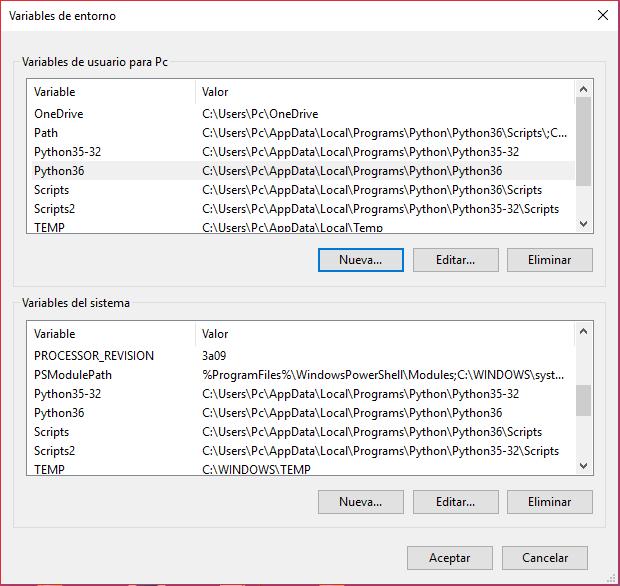
\includegraphics[width=\textwidth]{CapturasInstalacionPython/unnamed.png}
	\caption{Configuración de las variables de entorno en Windows.
	\label{fig:CapturasInstalacionPython/unnamed.png}}
\end{figure}

\section{Instalación del software Python}

Figura \ref{fig:CapturasInstalacionPython/unnamed.png}. Para este trabajo de fin de grado, se necesitaba desarrollar un software usando un programa de ordenador: Python. La última versión disponible a la hora de realizar dicho trabajo era la 3.6.4. Se ha utilizado además la versión de 64 bits, debido a que mi PC donde desarrollé el programa monta esta arquitectura de CPU.

A continuación, se explicará cómo descargar Python 3.6.4.

\begin{figure}[h!]
  	\centering
	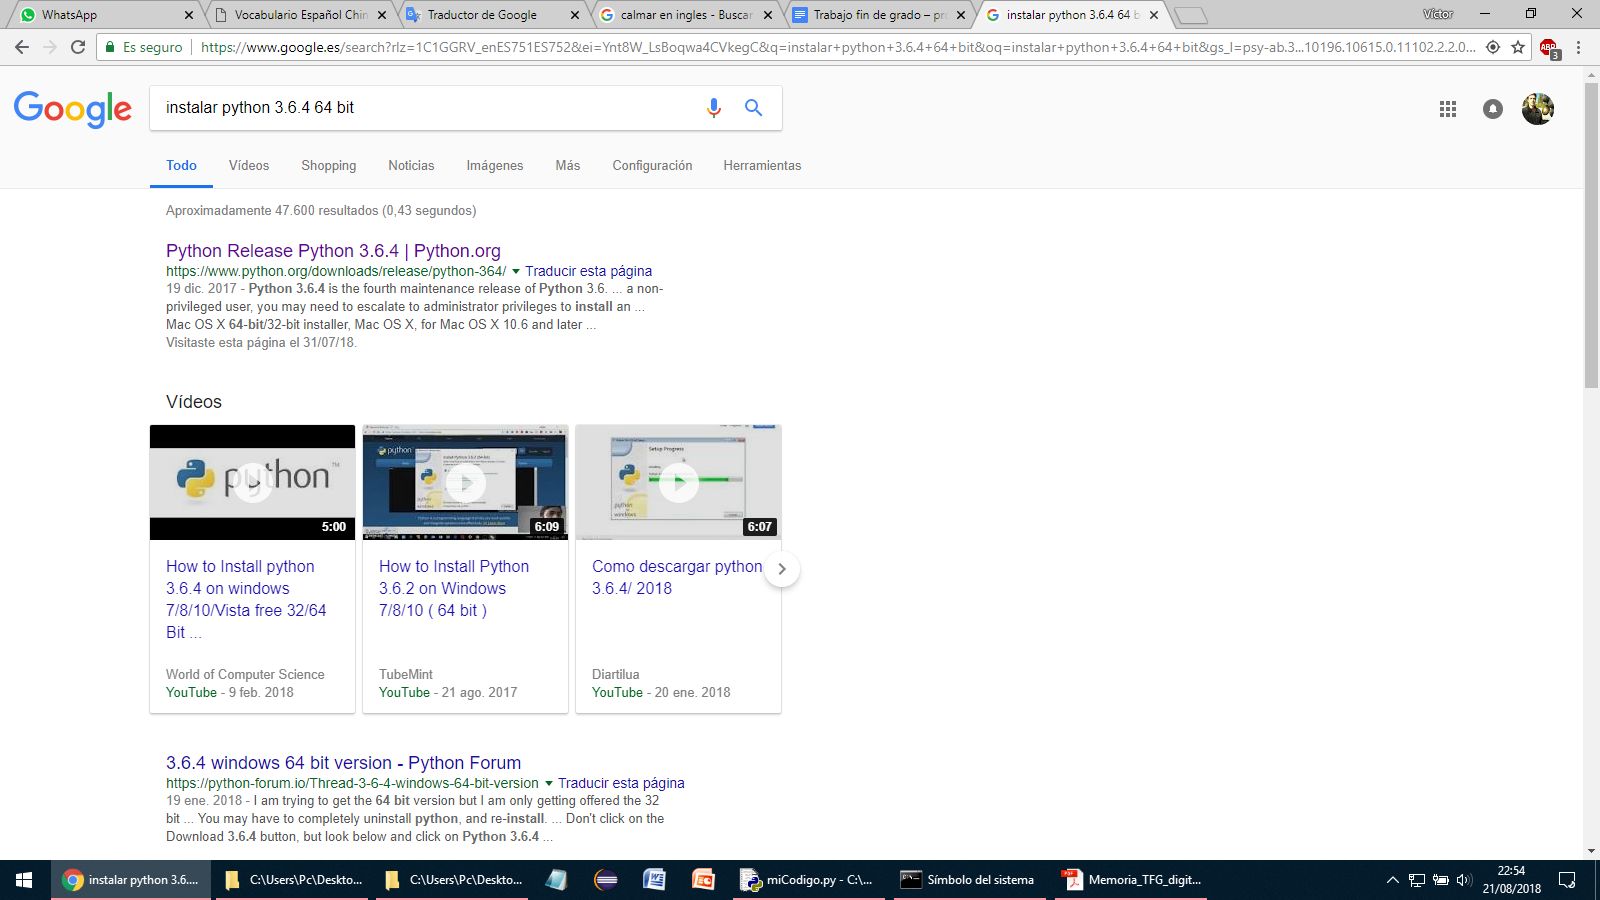
\includegraphics[width=\textwidth]{CapturasInstalacionPython/unnamed(1).png}
	\caption{Navegador Google Chrome donde se ha buscado la versión 3.6.4 de 64 bits de Python.
	\label{fig:CapturasInstalacionPython/unnamed(1).png}}
\end{figure}

Figura \ref{fig:CapturasInstalacionPython/unnamed(1).png}. Abrir un explorador de internet como Google Chrome, y buscar en Google ‘Instalar Python 3.6.4 64 bits’. Pinchar en el resultado ‘Python Release Python 3.6.4 | Python.org’.\\[20pt]

\begin{figure}[h!]
  	\centering
	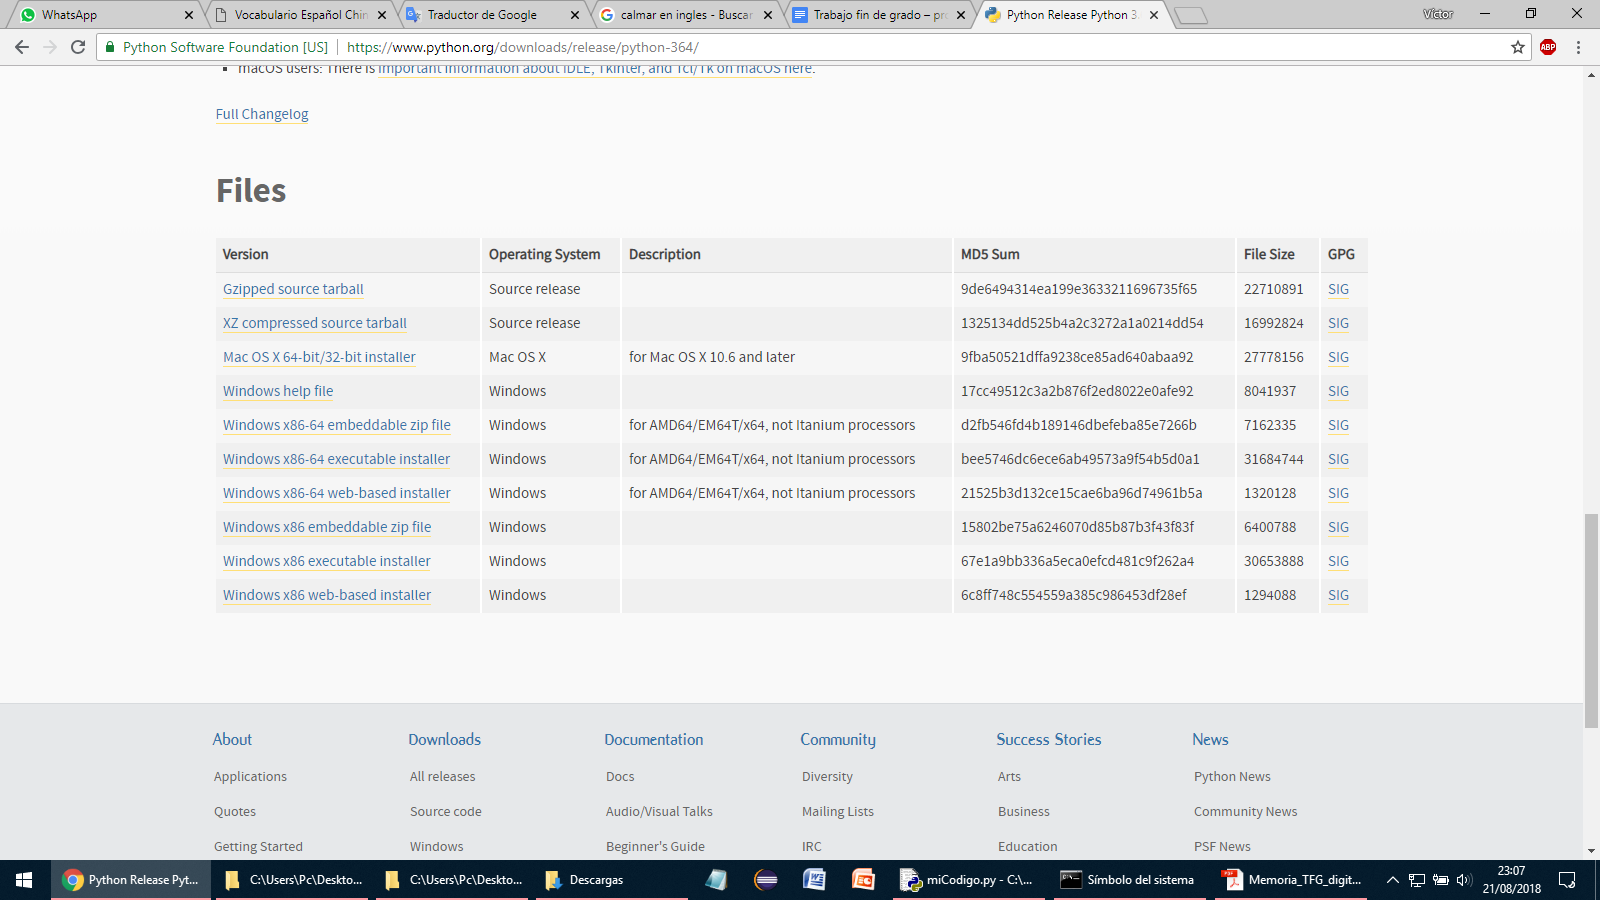
\includegraphics[width=\textwidth]{CapturasInstalacionPython/unnamed(2).png}
	\caption{Archivos de la versión elegida de Python.
	\label{fig:CapturasInstalacionPython/unnamed(2).png}}
\end{figure}

Figura \ref{fig:CapturasInstalacionPython/unnamed(2).png}. Una vez se haya accedido a esa página oficial de Python, realizar scroll hacia abajo para acceder a los archivos disponibles de esa versión de Python a descargar en el PC.\\[20pt]

\begin{figure}[h!]
  	\centering
	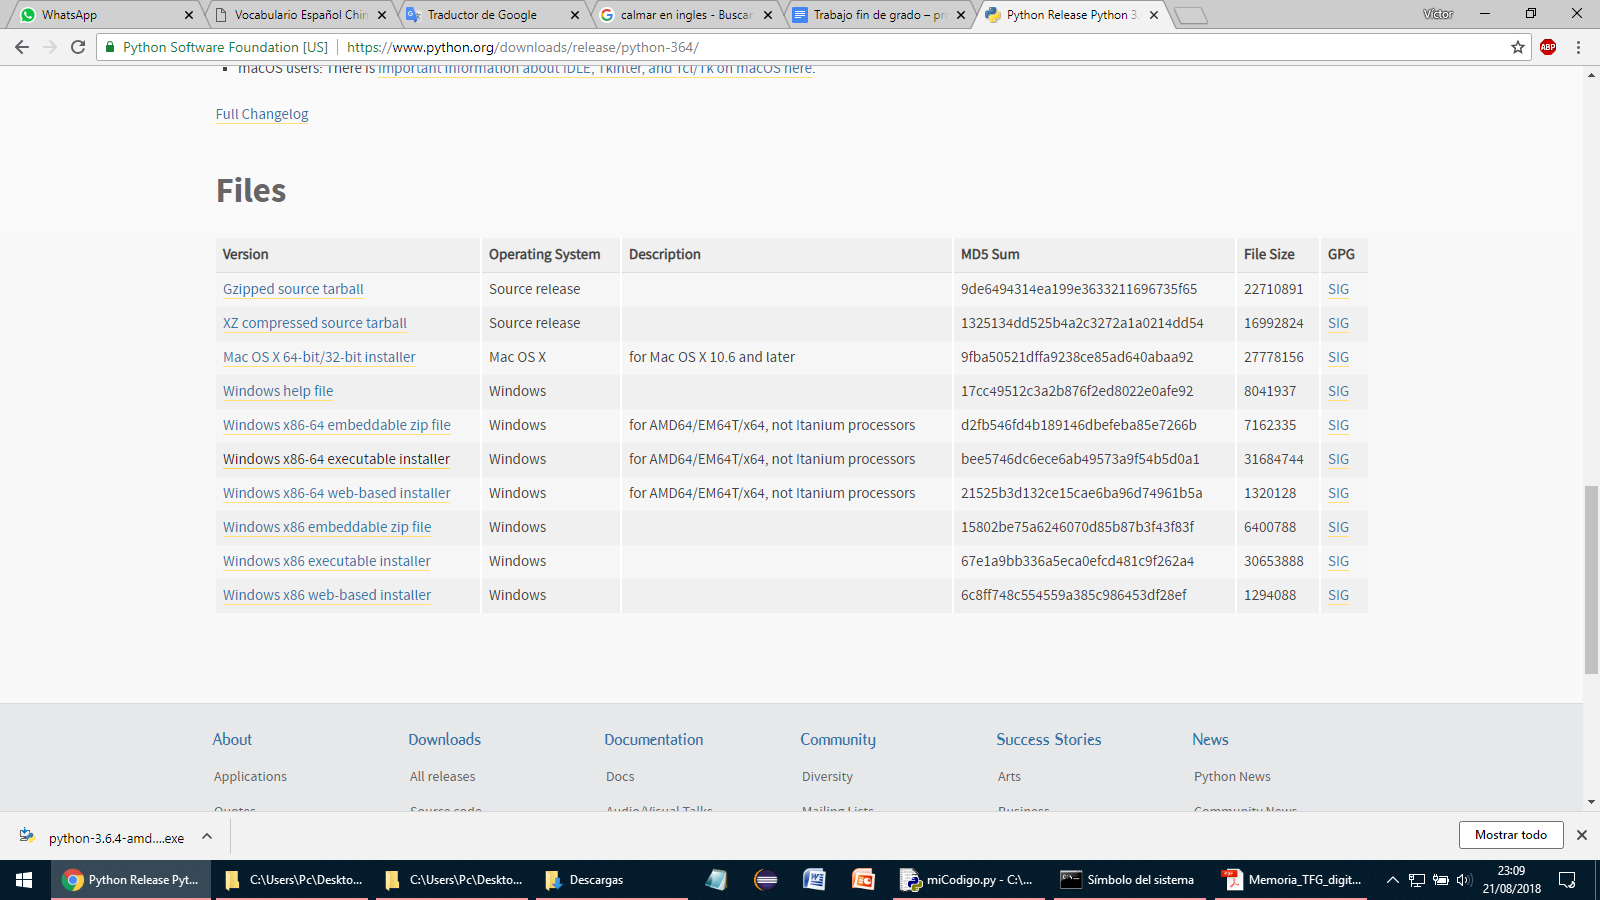
\includegraphics[width=\textwidth]{CapturasInstalacionPython/unnamed(3).png}
	\caption{Descarga del archivo ejecutable de Python en el sistema.
	\label{fig:CapturasInstalacionPython/unnamed(3).png}}
\end{figure}

Figura \ref{fig:CapturasInstalacionPython/unnamed(3).png}. Pinchar en ‘Windows x86-64 executable installer’ para descargar en el PC el instalador de Python, el cual se encargará de instalar este programa. La descarga se completará en cinco segundos. Pinchar en el archivo ‘EXE’ mostrado en la esquina inferior izquierda para abrir el instalador de Python.\\[20pt]

\begin{figure}[h!]
  	\centering
	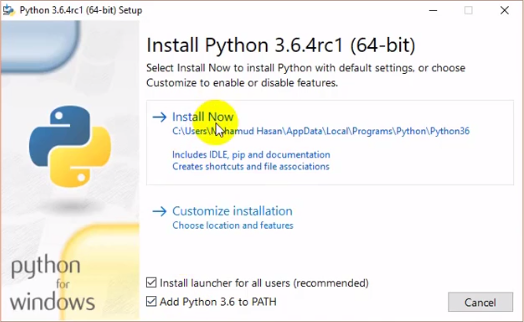
\includegraphics[width=\textwidth]{CapturasInstalacionPython/unnamed(4).png}
	\caption{Instalador de Python.
	\label{fig:CapturasInstalacionPython/unnamed(4).png}}
\end{figure}

Figura \ref{fig:CapturasInstalacionPython/unnamed(4).png}. Aparecerá esta ventana de instalación. A no ser que se desee agregar manualmente las variables de entorno de Python (con el fin de poder ejecutar Python desde la consola de comandos de Windows), hacer clic en ‘Add Python 3.6 to PATH’. El propio instalador llevará a cabo este procedimiento. A continuación, hacer clic en ‘Install Now’.\\[20pt]

\begin{figure}[h!]
  	\centering
	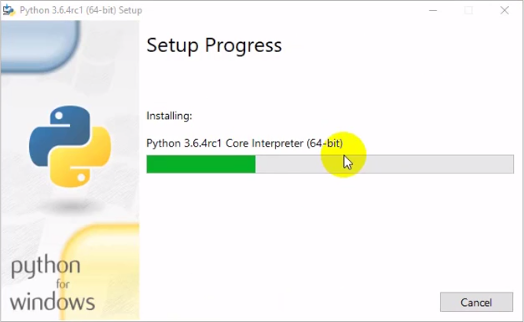
\includegraphics[width=\textwidth]{CapturasInstalacionPython/unnamed(5).png}
	\caption{Instalación de Python en curso.
	\label{fig:CapturasInstalacionPython/unnamed(5).png}}
\end{figure}

Figura \ref{fig:CapturasInstalacionPython/unnamed(5).png}. Se instalará Python en el sistema. Hay que esperar unos minutos para que este procedimiento se complete (cuando la barra verde se llene por completo).\\[20pt]

\begin{figure}[h!]
  	\centering
	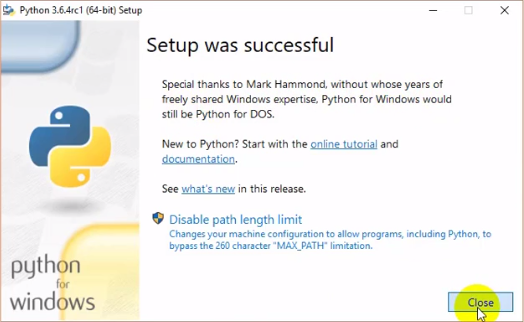
\includegraphics[width=\textwidth]{CapturasInstalacionPython/unnamed(6).png}
	\caption{Instalación de Python exitosa.
	\label{fig:CapturasInstalacionPython/unnamed(6).png}}
\end{figure}

Figura \ref{fig:CapturasInstalacionPython/unnamed(6).png}. Cuando finalice correctamente la instalación, se mostrará en la ventana del instalador ‘Setup was successful’. Hacer clic en ‘Close’ para cerrar el instalador.\\[20pt]

\begin{figure}[h!]
  	\centering
	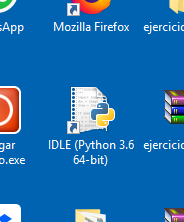
\includegraphics[scale=1]{CapturasInstalacionPython/unnamed(7).png}
	\caption{Icono en el escritorio para abrir Python.
	\label{fig:CapturasInstalacionPython/unnamed(7).png}}
\end{figure}

Figura \ref{fig:CapturasInstalacionPython/unnamed(7).png}. El icono de Python debería aparecer en el escritorio. Hacer doble clic para abrir el programa.\\[20pt]

\begin{figure}[h!]
  	\centering
	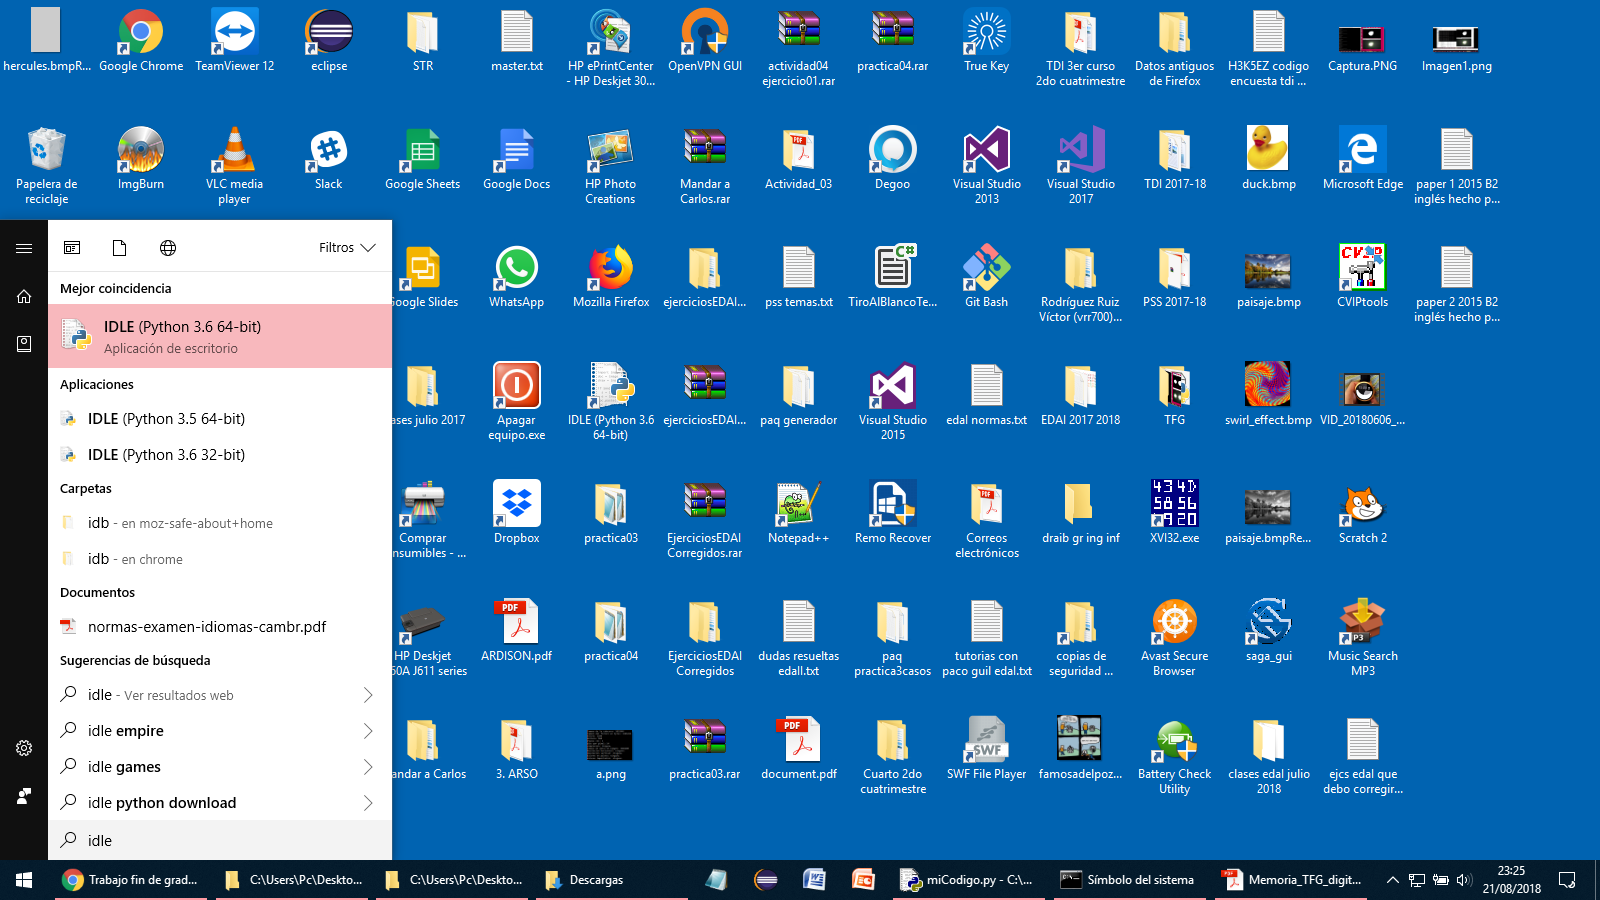
\includegraphics[width=\textwidth]{CapturasInstalacionPython/unnamed(8).png}
	\caption{Menú Inicio de Windows, buscando Python desde él.
	\label{fig:CapturasInstalacionPython/unnamed(8).png}}
\end{figure}

Figura \ref{fig:CapturasInstalacionPython/unnamed(8).png}. Si no aparece el icono de Python en el escritorio, hacer clic en el logotipo (o bandera) de Windows mostrado en la esquina inferior izquierda de la pantalla, y teclear ‘idle’. Debería ya aparecer en el buscador de programas ‘IDLE (Python 3.6 64-bit)’. Hacer clic ahí para abrirlo.\\[20pt]

\begin{figure}[h!]
  	\centering
	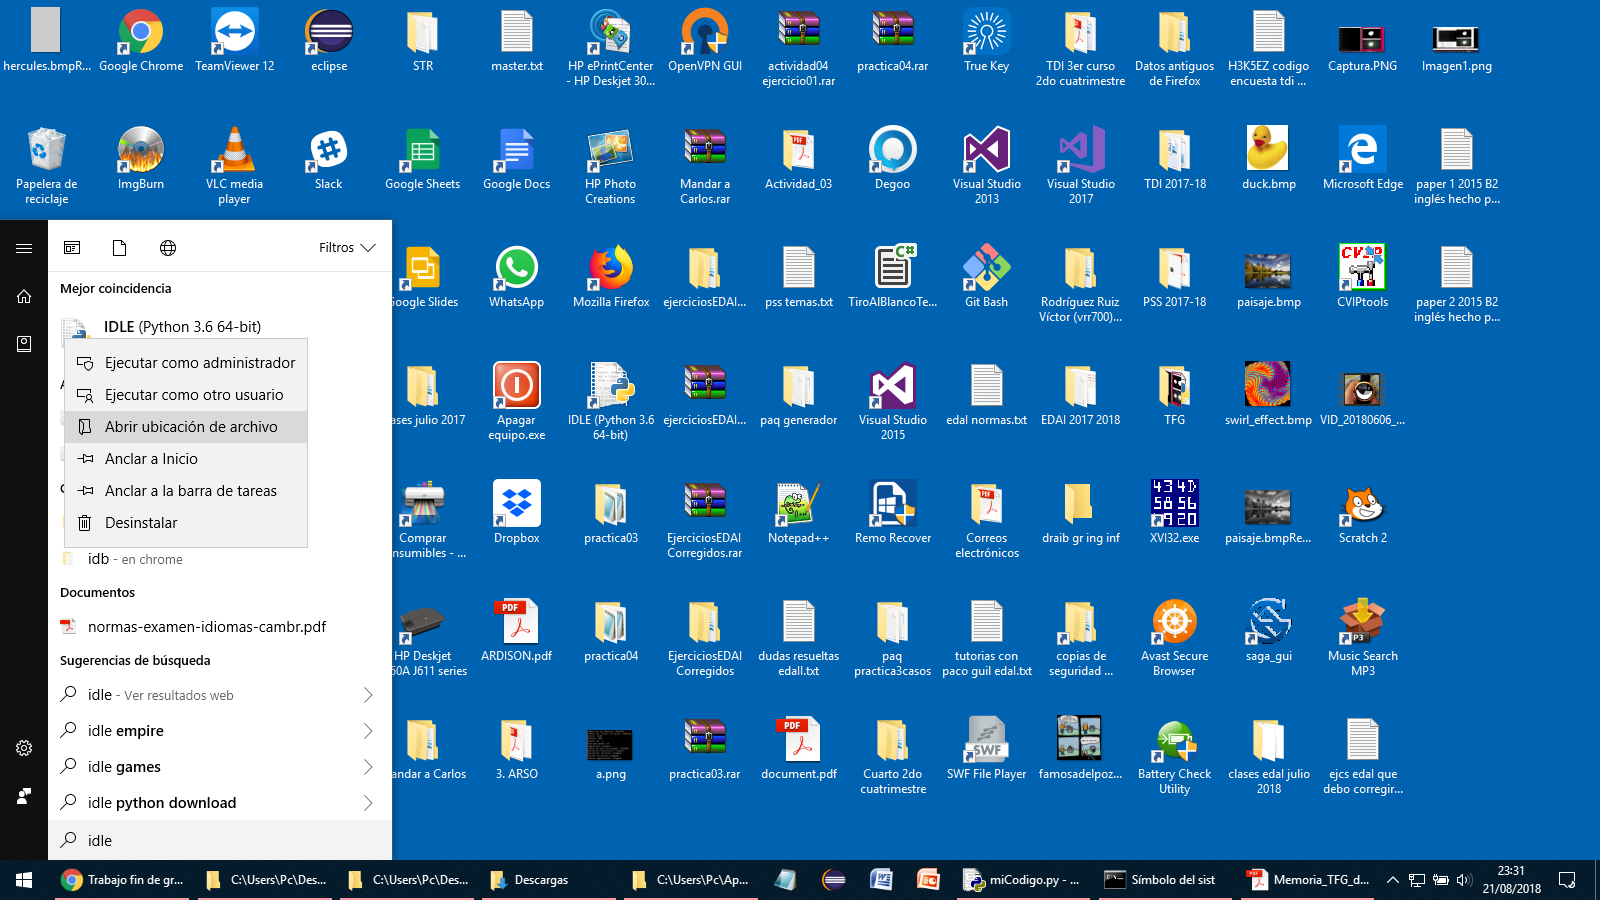
\includegraphics[width=\textwidth]{CapturasInstalacionPython/unnamed(9).png}
	\caption{Abrir la ubicación del archivo Python en el sistema.
	\label{fig:CapturasInstalacionPython/unnamed(9).png}}
\end{figure}

Figura \ref{fig:CapturasInstalacionPython/unnamed(9).png}. En el caso de querer agregar el icono del programa al escritorio (si no lo estaba), desde esa misma pantalla del buscador de programas, situar el cursor sobre el programa, hacer clic con el botón derecho del ratón, y seleccionar ‘Abrir ubicación de archivo’. Se mostrará la ubicación exacta del archivo en el sistema, abriéndose la ventana del explorador de archivos de Windows.\\[20pt]

\begin{figure}[h!]
  	\centering
	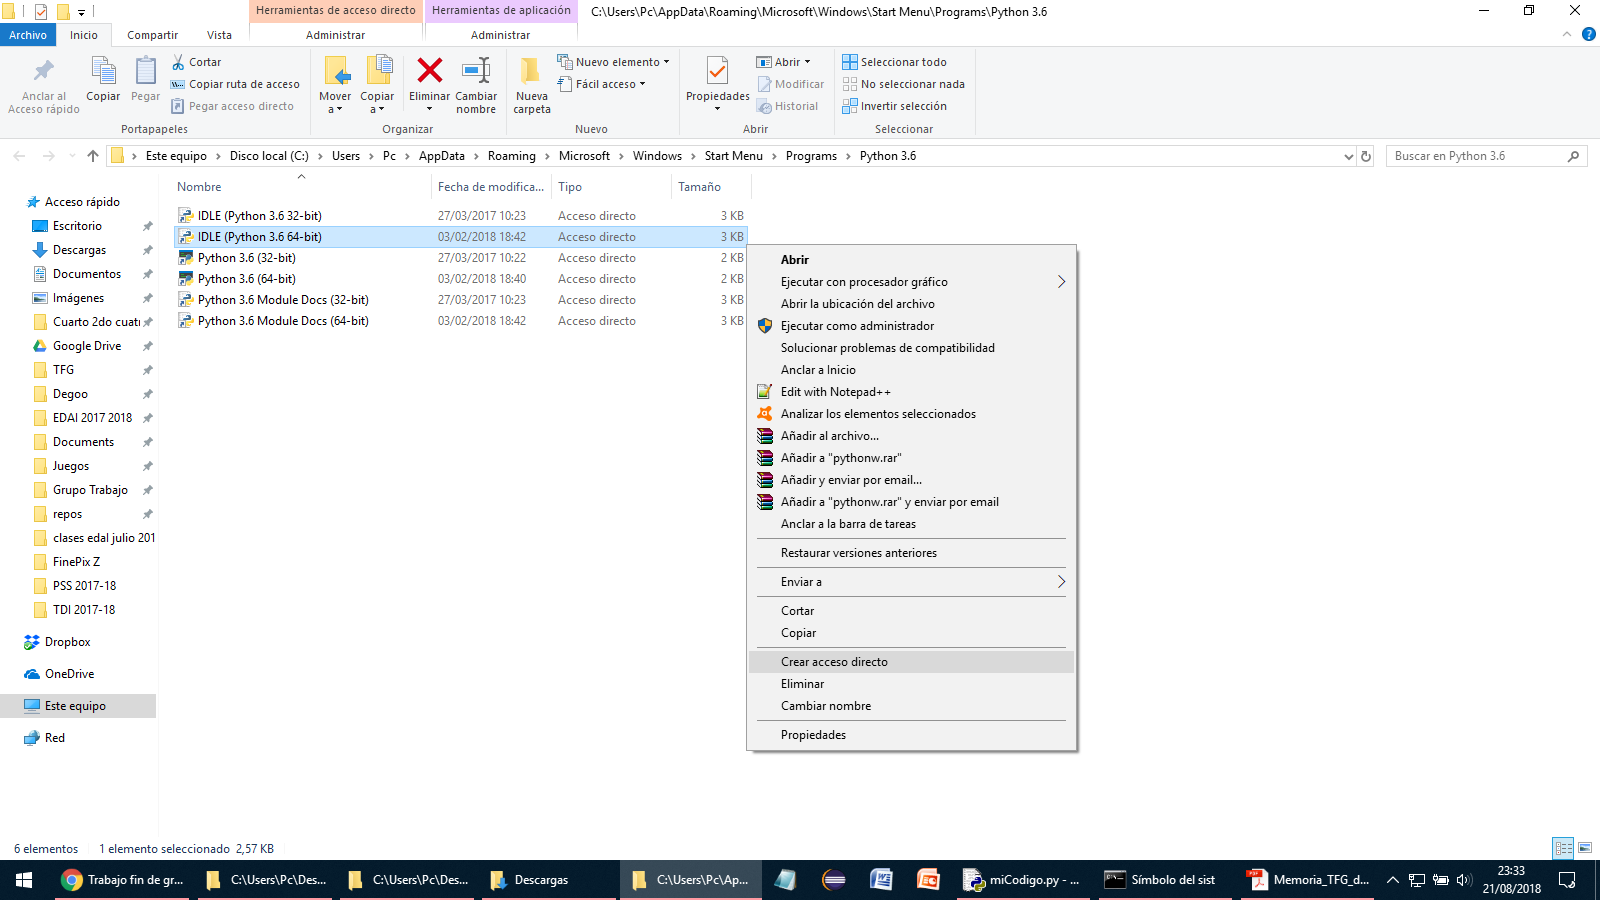
\includegraphics[width=\textwidth]{CapturasInstalacionPython/unnamed(10).png}
	\caption{Creando un acceso directo de Python.
	\label{fig:CapturasInstalacionPython/unnamed(10).png}}
\end{figure}

Figura \ref{fig:CapturasInstalacionPython/unnamed(10).png}. Desde esa ventana, y haciendo clic con el botón derecho del ratón sobre el programa (acceso directo) ‘IDLE (Python 3.6 64-bit)’, seleccionar desde el menú contextual ‘Crear acceso directo’. Se creará un nuevo acceso directo a ese programa, en esta misma ventana, con nombre ‘IDLE (Python 3.6 64-bit) (2)’.\\[20pt]

\begin{figure}[h!]
  	\centering
	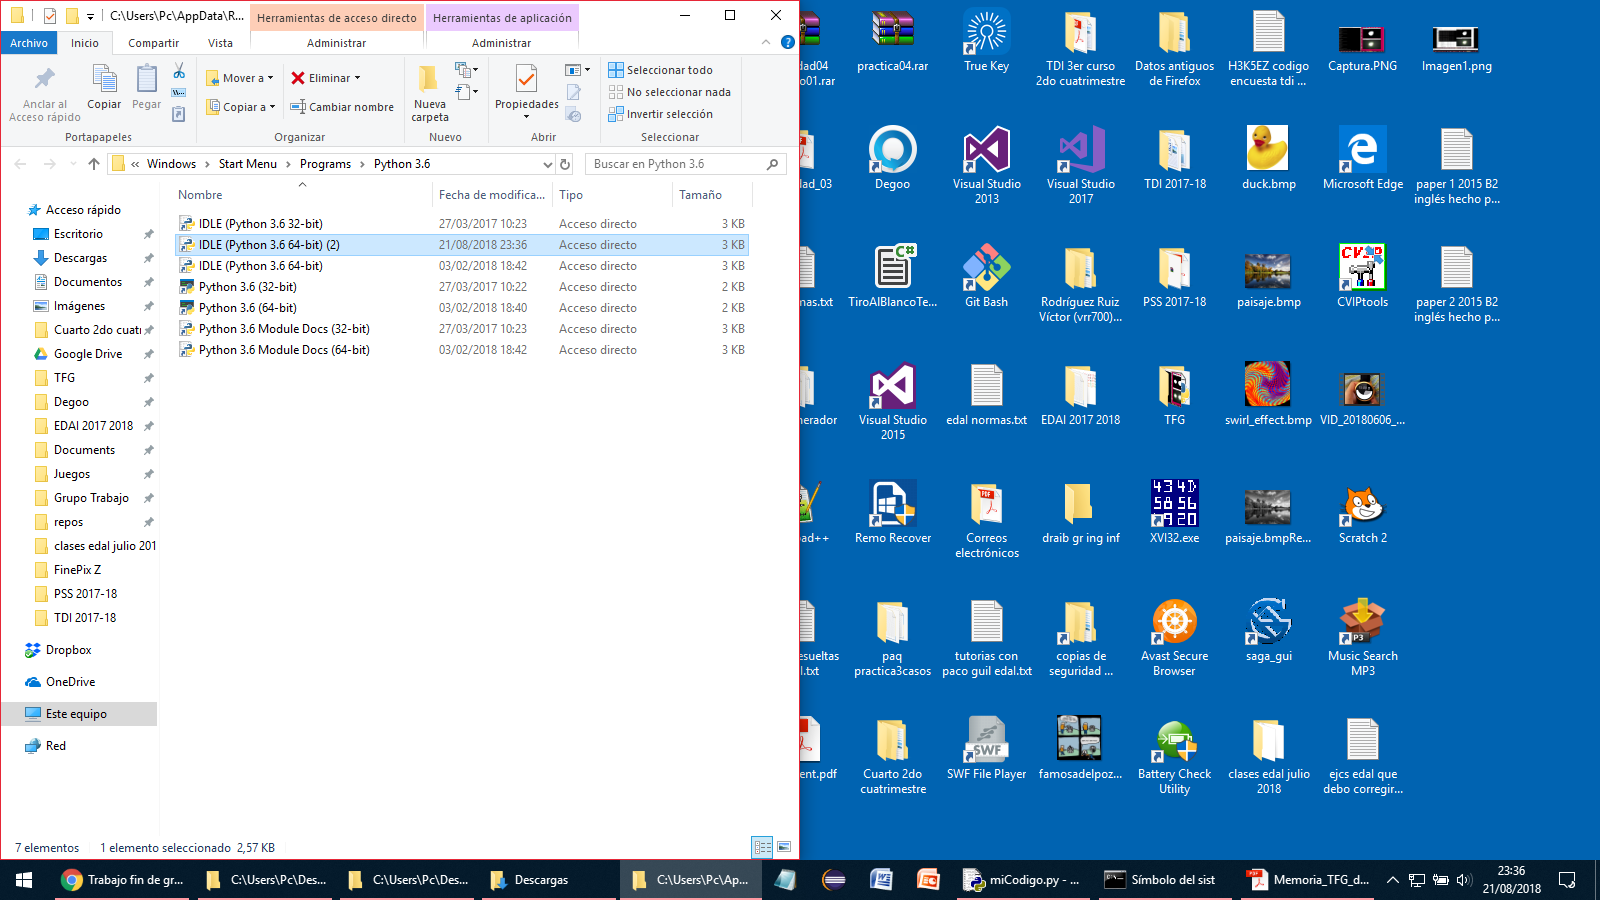
\includegraphics[width=\textwidth]{CapturasInstalacionPython/unnamed(11).png}
	\caption{Arrastrar el acceso directo de Python creado previamente al escritorio.
	\label{fig:CapturasInstalacionPython/unnamed(11).png}}
\end{figure}

Figura \ref{fig:CapturasInstalacionPython/unnamed(11).png}. Reducir el tamaño de la ventana, de forma parecida a la mostrada en esta captura de pantalla. Tras esto, simplemente habría que arrastrar y soltar este acceso directo ‘IDLE (Python 3.6 64-bit) (2)’ desde esa ventana al escritorio. Así, ya se tiene el programa en el escritorio.\\[20pt]

\section{Cómo usar el software}

Para usar y ejecutar el software en el PC descrito en este informe, especialmente por primera vez, se siguen las siguientes instrucciones:

\# Helióstatos

--- Cómo abrir y ejecutar el proyecto de caracterización de helióstatos ---

Nota: el código de este proyecto se realizó mediante el programa Python e IDLE 3.6.4.

1. Acceder a la página Web donde se ubica el proyecto: \url{https://github.com/VictorRodri/Heliostatos}.

2. En ella, hacer clic en el botón verde 'Clone or download' \textgreater 'Download ZIP'.

3. El proyecto se descargará en el disco duro del equipo, generalmente en 'Documentos' \textgreater 'Descargas'. De lo contrario, especificar en qué ruta exacta del equipo se realizará la descarga.

4. Descomprimir el proyecto descargado previamente, usando un software como WinRAR: \url{https://www.winrar.es/descargas}.

5. Instalar la última versión de Python desde su página Web oficial: \url{https://www.python.org/downloads/}.

6. Abrir la terminal de comandos de Windows. Para ello, hacer clic en 'Inicio' \textgreater 'Ejecutar'. En la ventana que aparecerá, escribir en el cuadro de texto 'cmd' y pulsar Enter.

7. La terminal mostrará la ruta o directorio del sistema donde se ubica usted actualmente, como \verb|C:\Users\Pc>|. Ir navegando hasta encontrar el directorio que contiene el proyecto descomprimido previamente. Para acceder a una carpeta, escribir 'cd NombreCarpeta' y pulsar Enter. Para salir del directorio actual, escribir 'cd ..'.

8. Una vez se haya navegado al directorio que contiene el proyecto, ejecutarlo con el comando \verb|estimacion_potencia.py Videos/varios_heliostatos.mp4 50 50|, siendo respectivamente el nombre del proyecto '.py' con el software ejecutable, el directorio que contiene el vídeo de helióstatos a ser procesado, y el ancho y alto mínimos del helióstato para su detección y análisis.

9. Durante aproximadamente un minuto, se ejecutará el software que consistirá en medir la radiación de energía que proyecta cada helióstato. Concretamente, la energía se calcula como la sumatoria de los cuadrados de cada componente BGR del helióstato. Aparecerán estos resultados en tiempo de ejecución en la consola, para cada fotograma del vídeo de helióstatos.

10. Si desea cancelar la ejecución del software, pulsar 'Ctrl+C'.

\section{Diagrama de flujo}

El funcionamiento del código de helióstatos mediante la representación de un diagrama de flujo es el siguiente:

\begin{figure}[h!]
  	\centering
	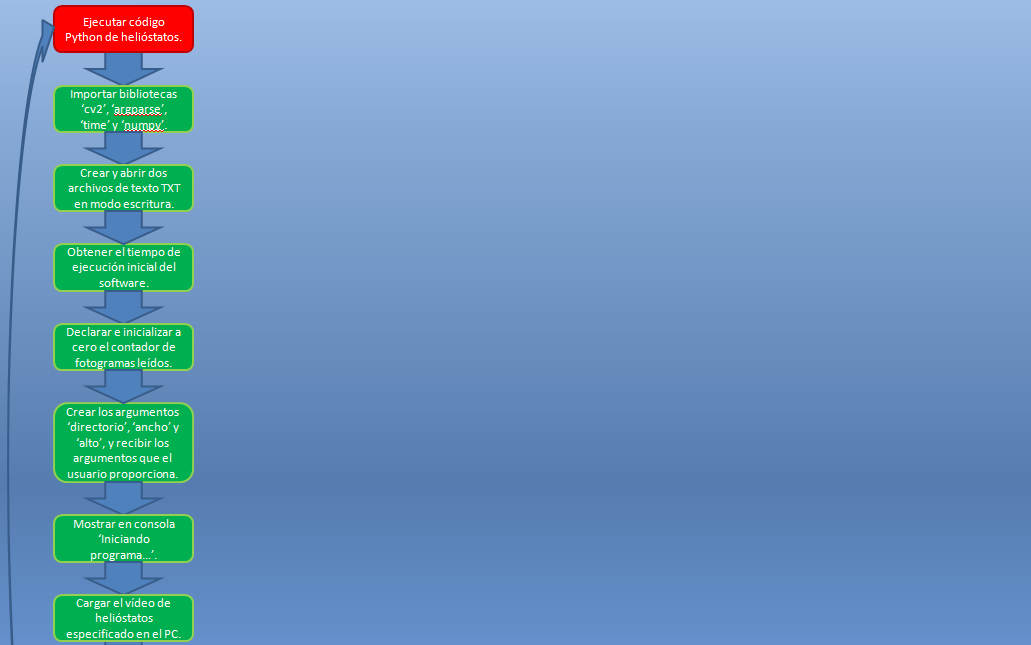
\includegraphics[width=\textwidth]{DiagramaFlujoSoftwareTFG/diagramaFlujo1.PNG}
	\caption{Diagrama de flujo, parte 1.
	\label{fig:DiagramaFlujoSoftwareTFG/diagramaFlujo1.PNG}}
\end{figure}

\begin{figure}[h!]
  	\centering
	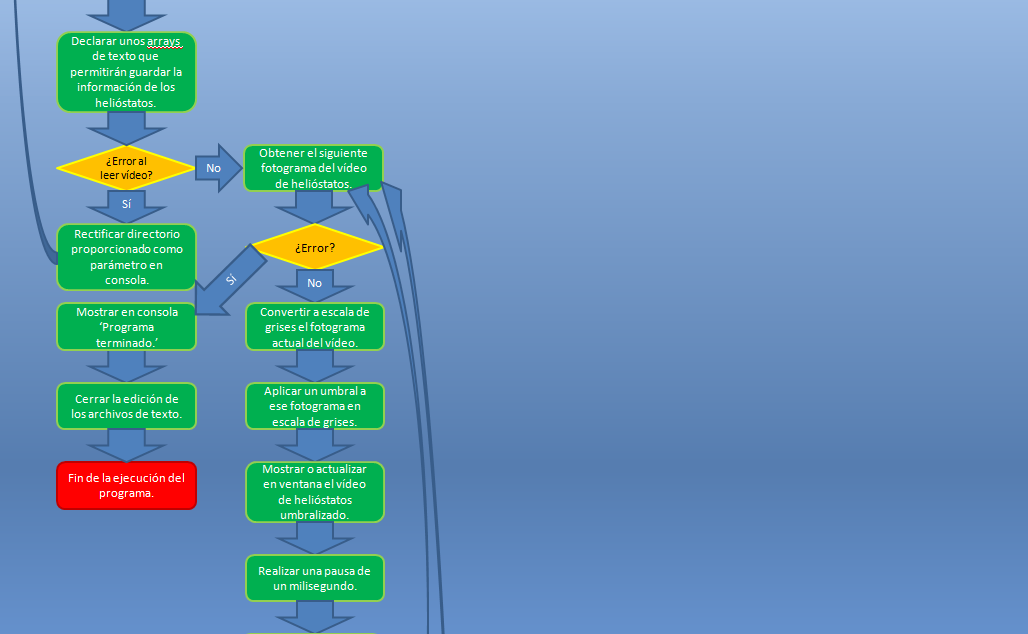
\includegraphics[width=\textwidth]{DiagramaFlujoSoftwareTFG/diagramaFlujo2.PNG}
	\caption{Diagrama de flujo, parte 2.
	\label{fig:DiagramaFlujoSoftwareTFG/diagramaFlujo2.PNG}}
\end{figure}

\begin{figure}[h!]
  	\centering
	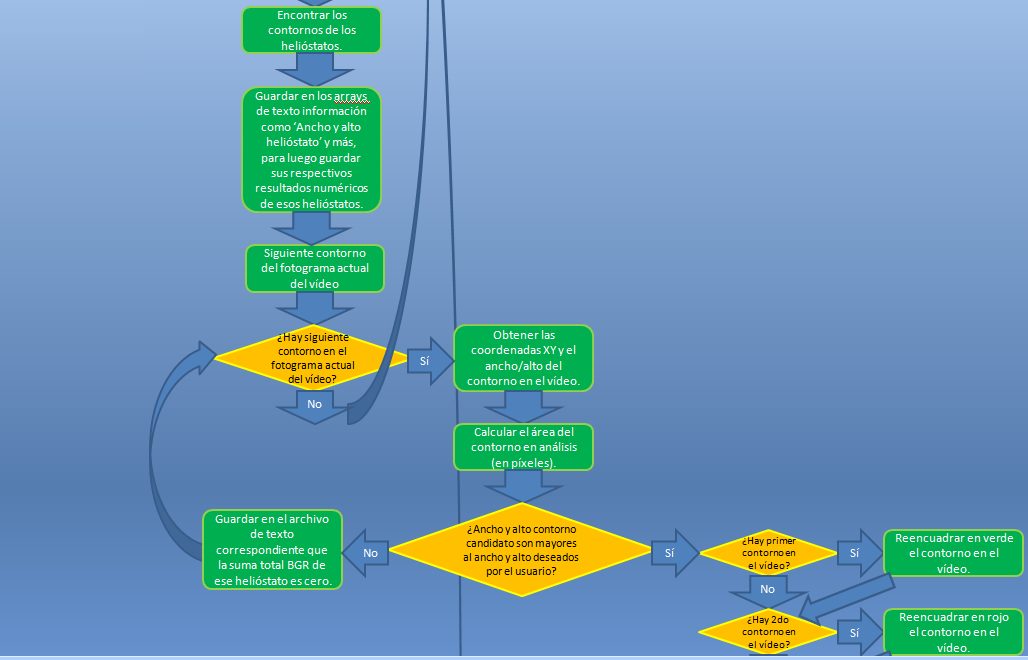
\includegraphics[width=\textwidth]{DiagramaFlujoSoftwareTFG/diagramaFlujo3.PNG}
	\caption{Diagrama de flujo, parte 3.
	\label{fig:DiagramaFlujoSoftwareTFG/diagramaFlujo3.PNG}}
\end{figure}

\begin{figure}[h!]
  	\centering
	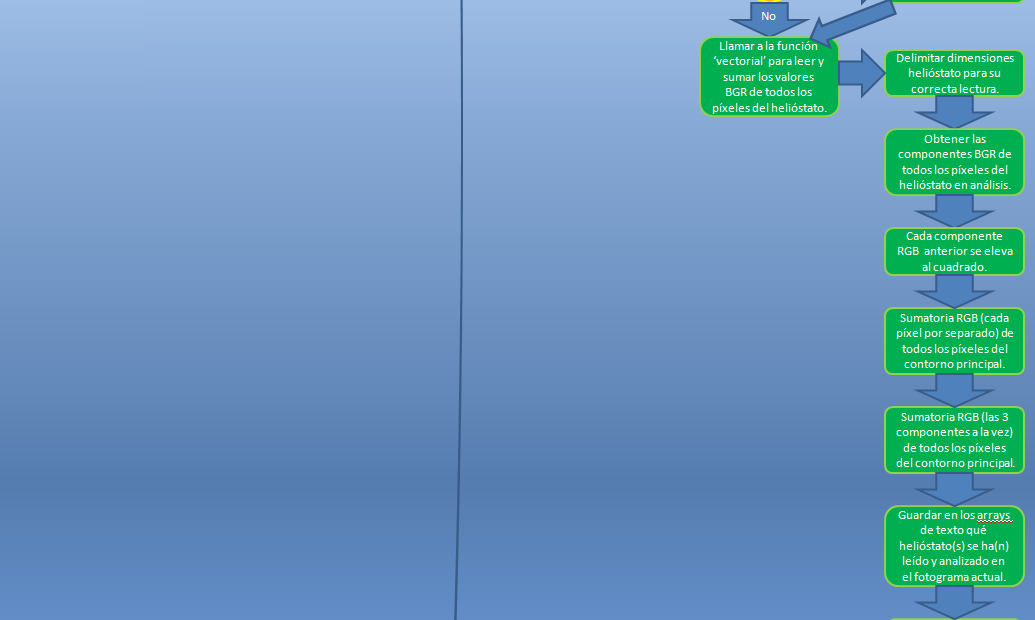
\includegraphics[width=\textwidth]{DiagramaFlujoSoftwareTFG/diagramaFlujo4.PNG}
	\caption{Diagrama de flujo, parte 4.
	\label{fig:DiagramaFlujoSoftwareTFG/diagramaFlujo4.PNG}}
\end{figure}

\begin{figure}[h!]
  	\centering
	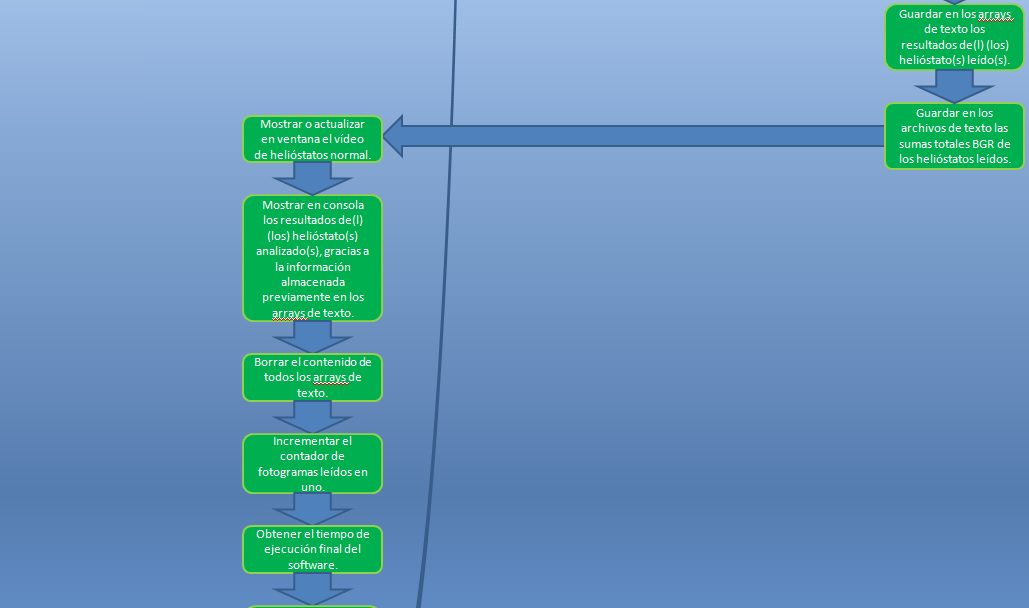
\includegraphics[width=\textwidth]{DiagramaFlujoSoftwareTFG/diagramaFlujo5.PNG}
	\caption{Diagrama de flujo, parte 5.
	\label{fig:DiagramaFlujoSoftwareTFG/diagramaFlujo5.PNG}}
\end{figure}

\begin{figure}[h!]
  	\centering
	
\includegraphics[width=\textwidth]{DiagramaFlujoSoftwareTFG/diagramaFlujo6.PNG}
	\caption{Diagrama de flujo, parte 6.
	\label{fig:DiagramaFlujoSoftwareTFG/diagramaFlujo6.PNG}}
\end{figure}

\section{Funcionamiento del software y código}

El software consiste en la lectura y procesamiento de un vídeo guardado en el disco duro del ordenador personal y en formato MP4. El vídeo es de un conjunto de helióstatos que van entrando uno por uno en un panel solar y fusionándose todos entre sí. Y tras esto, los helióstatos van saliendo uno por uno de ese panel solar, hasta que no quede ninguno.

El código desarrollado es el siguiente:\\[20pt]

\begin{lstlisting}
# Bibliotecas requeridas para este software.
import cv2
import argparse
import time
import numpy as np
\end{lstlisting}

Para que funcione todo el código expuesto y elaborado a continuación, hay que importar en este caso las librerías \verb|cv2|, \verb|argparse|, \verb|time| y \verb|numpy| (esta última se ha asignado un nombre propio: \verb|np|).

\verb|cv2| permite el uso de distintas funcionalidades de Python. En este proyecto, se ha usado para la captura y lectura de un vídeo guardado en el sistema, convertirlo de color a escala de grises, aplicarle un umbral (diferenciar solo dos niveles de grises: u oscuros o claros), mostrar el vídeo original y umbralizado en pantalla y en reproducción (conforme el programa lo va analizando fotograma a fotograma), realizar pausas (breves o prolongadas) de la ejecución del código, detectar y localizar contornos (helióstatos) en el vídeo, calcular el ancho y alto en píxeles de los contornos, así como sus valores de área, calcular la sumatoria parcial y total de los valores de todos los píxeles BGR al cuadrado de cada helióstato, y dibujar un rectángulo verde o de otro color alrededor del contorno en el vídeo.

\verb|argparse| es usado para proporcionar distintos parámetros desde la consola de Windows al ejecutar este código, de tal forma que el programa sea ejecutado de una forma u otra según la petición de datos del usuario, como las dimensiones del helióstato que el programa analizará, y así ignorar los helióstatos con dimensiones ajenas a las deseadas por el usuario.

\verb|time| permite medir tiempos de ejecución de todo el código o de fragmentos de código, en segundos. Se utilizará para medir la tasa de ‘frames’ (fotogramas) por segundo de la lectura y procesado del vídeo de helióstatos, y así comprobar la eficiencia de la ejecución del programa.

\verb|numpy| permite el manejo de arrays o vectores con el fin de recorrer y analizar una serie de datos en secuencia, como una matriz de dos dimensiones y con muchos valores numéricos guardados. Además, usar \verb|numpy| para dicho fin es mucho más eficiente que otros métodos de análisis de datos en secuencia que no sean en arrays o vectores, como los típicos bucles ‘for’.\\[20pt]

\begin{lstlisting}
# Crear y abrir los siguientes archivos de texto en modo
# escritura.
f1 = open("SumasBGRHeliostatosVerdes.txt", "w")
f2 = open("SumasBGRHeliostatosRojos.txt", "w")
\end{lstlisting}

En el directorio del sistema donde se está ejecutando este software, se crearán los ficheros de texto "SumasBGRHeliostatosVerdes.txt" y "SumasBGRHeliostatosRojos.txt" y se escribirán informaciones en ellos (significado del parámetro \verb|w|). Si ya existían estos ficheros en el sistema, serán sobreescritos por los nuevos.\\[20pt]

\begin{lstlisting}
start\_time = time.time() # Obtener el tiempo de ejecución
# inicial de este programa.
frame\_counter = 0 # Contador de fotogramas totales del vídeo.
# Se irá incrementando progresivamente en líneas de código
# posteriores.
\end{lstlisting}

Obtener en segundos el tiempo de ejecución inicial del programa. Inicial porque esta línea de código se ubica en el comienzo del software. Declarar e inicializar a cero un contador de fotogramas del vídeo. Ambos datos serán usados para calcular los FPS (fotogramas por segundo) del vídeo de helióstatos, al final de este código.\\[20pt]

\begin{lstlisting}
# Argumentos o parámetros necesarios para ejecutar este programa
# a través de la consola de Windows.
parser = 
argparse.ArgumentParser(description='Parametros del programa.')
# Dar un nombre al conjunto de parámetros y asignarlo a la
# variable 'parser'.
parser.add_argument('directorioVideoHeliostatosCargar', type=str)
# Crear el argumento 1: ruta o directorio del vídeo a cargar en
# el PC.
parser.add_argument('anchoMinimoHeliostato', type=int) # Crear el 
# argumento 3: ancho mínimo del helióstato para su análisis.
parser.add_argument('altoMinimoHeliostato', type=int) # Crear
# el argumento 4: alto mínimo del helióstato para su análisis.
parser.add_argument('umbralVideoHeliostatos', type=int) # Crear
# el argumento 5: umbral o nivel de color mínimo del vídeo de
# helióstatos a partir del cual podría estar detectándose un
# helióstato.
parser.add_argument('numeroHeliostatosAnalizar', type=int)
# Crear el argumento 6: número máximo de helióstatos a detectar y
# analizar en cada fotograma del vídeo de helióstatos.
args = parser.parse_args() # Devuelve información de los
# parámetros definidos previamente.
\end{lstlisting}

Permite que a la hora de ejecutar el programa desde la terminal de comandos de Windows, solicite al usuario la ruta del vídeo a cargar del sistema, el ancho y alto mínimos del helióstato para ser detectado y analizado por el programa, el umbral (o tonalidad del color) del vídeo a partir del cual el programa detectará los helióstatos, y el número máximo de helióstatos que el programa deberá detectar y analizar, para cada fotograma del vídeo de helióstatos. Por ejemplo: \verb|C:\Users\Pc\Desktop\TFG>miCodigo.py Videos/varios_heliostatos.mp4 50 50 127 2|.

\verb|parser = argparse.ArgumentParser(description='Parametros del programa.')|. Esta línea de código permite asignar un conjunto de parámetros o argumentos y de darles un nombre. Es guardado en la variable \verb|parser|.

Partiendo de la anterior variable \verb|parser|, se van designando los distintos argumentos, junto a sus nombres y tipos, como cadena o entero (según si la entrada del parámetro hay que escribir letras y/o caracteres, o simplemente números).

\verb|args = parser.parse_args()|. Permite que, desde la variable \verb|args|, cargar el argumento concreto, almacenado previamente cuando el programa solicitó al usuario los argumentos. Por ejemplo, si se desea comprobar cuál fue el ancho del helióstato que el usuario solicitó por parámetro en la consola, se cargará y obtendrá el segundo argumento con la línea de código siguiente: \verb|args.anchoMinimoHeliostato|. Así, el programa realizará las medidas y operaciones oportunas de acuerdo al valor de este parámetro deseado por el usuario.\\[20pt]

\begin{lstlisting}
# Mostrar en la consola este aviso de cuando se va a ejecutar el
# programa.
print("")
print("Iniciando programa...")
print("")
\end{lstlisting}

Al iniciar la ejecución del programa, mostrará por consola que se ha iniciado su ejecución, con el aviso ‘Iniciando programa…’. Este aviso solo aparecerá una vez durante toda su ejecución.\\[20pt]

\begin{lstlisting}
# Leer secuencia de imágenes del vídeo a partir del directorio
# especificado por parámetro.
camara = cv2.VideoCapture(args.directorioVideoHeliostatosCargar)
\end{lstlisting}

Partiendo del directorio especificado por el usuario, el programa leerá y cargará el archivo concreto, que deberá ser el vídeo de helióstatos. De lo contrario, la ejecución del programa no se realizará correctamente.\\[20pt]

\begin{lstlisting}
# Declarar estos arrays con el fin de almacenar toda la
# información sobre los resultados de los helióstatos analizados
# en el vídeo de helióstatos.
# Además, son usados especialmente con el fin de mostrar, para
# cada información, hasta dos resultados distintos (uno para cada
# helióstato) en una misma línea de texto, en la consola.
heliostato = []
anchoAlto = []
areaTotal = []
sumaBGRparcial = []
sumaBGRtotal = []
\end{lstlisting}

Arrays que permiten almacenar y mostrar en consola toda la información y resultados sobre los helióstatos analizados en el vídeo de helióstatos. El uso concreto de estos arrays se debe a que con ellos es posible mostrar en consola y para cada información, hasta dos resultados distintos (uno para cada helióstato) en una misma línea de texto, de la forma que se explicará posteriormente. Así se evita el uso de demasiadas líneas de texto en la consola, y compactar toda la información posible en una sola. Estos arrays son vaciados una vez que se haya guardado la información correspondiente al helióstato (o helióstatos) del fotograma actual (en análisis) del vídeo de helióstatos, y posteriormente mostradas dichas informaciones de ese helióstato (o helióstatos) en consola. Todo este procedimiento se repite igual para los siguientes fotogramas de dicho vídeo de helióstatos.\\[20pt]

\begin{lstlisting}
# Iteración 'while True' para cada fotograma del vídeo, hasta
# completar todos los fotogramas y llegar al final del vídeo
# (cambiaría automáticamente de True a False y el bucle 'while'
# finaliza).
while True:
\end{lstlisting}

A partir de aquí y prácticamente hasta el final del código, todas las demás instrucciones se aplicarán para cada fotograma del vídeo de helióstatos.\\[20pt]
    
\begin{lstlisting}
    # Obtener frame. Para ello, se toma un fotograma del vídeo,
    # se guarda en 'frame', y si se ha hecho esta acción
    # correctamente, 'grabbed' valdrá true (verdadero), y
    # viceversa.
    (grabbed, frame) = camara.read()

    # Si se ha llegado al final del vídeo, romper la ejecución
    # de este bucle 'while' y finalizar el programa.
    if not grabbed:
        break
\end{lstlisting}

Estas líneas de código se encargarán de indicar al programa si quedan más fotogramas por leer o no del vídeo de helióstatos, y así saber hasta cuándo dicho programa se mantendría en ejecución. Primero, \verb|camara.read()| obtiene el fotograma actual del vídeo, y lo guarda en la variable \verb|frame|. Si se ha hecho esta acción correctamente (debido a que quedan más fotogramas por leer del vídeo y no se ha llegado al final del mismo), \verb|grabbed| (justo al lado izquierdo de \verb|frame|) valdrá \verb|true|, y viceversa. Si se ha llegado al final del vídeo, \verb|grabbed| valdrá \verb|false| (porque ya no quedan más fotogramas por leer), y romperá la ejecución del presente bucle \verb|while| para que deje de leer más fotogramas del vídeo y finalice la ejecución de este programa. Esta ruptura es producida porque se cumple la condición de \verb|if not grabbed|, así que desencadena la instrucción \verb|break|.\\[20pt]

\begin{lstlisting}
    # Convertir a escala de grises el fotograma actual del
    # vídeo. Para ello, con la variable 'frame' (fotograma del
    # vídeo) capturada anteriormente, se llama a la función
    # 'cv2.COLOR\_BGR2GRAY'.
    img = cv2.cvtColor(frame, cv2.COLOR\_BGR2GRAY)
    
    # Aplicar un umbral a ese fotograma del vídeo. Parámetros de
    # este método: imagen fuente en escala de grises, valor de 
    # umbral para clasificar los valores de píxeles de esa imagen,
    # valor máximo a ser representado si el valor del píxel
    # supera al valor del umbral, aplicar un tipo concreto de
    # umbralización (0 porque no se desea hacer esto).
    # NOTA: la variable "ret" que recibe como resultado en este
    # método no es usada en este programa así que se puede
    # ignorar, esto es debido a que no se está aplicando
    # umbralización de Otsu.
    ret, thresh =
    cv2.threshold(img, args.umbralVideoHeliostatos, 255, 0)
    
    cv2.imshow("Camara2", thresh) # Mostrar vídeo umbralizado en
    # una ventana.
    cv2.waitKey(1) # El programa hará una pequeña pausa (1
    # milisegundo) para que de tiempo a que se muestren los
    # vídeos y fotogramas en las dos ventanas que se han creado
    # en este código para tal fin.

    # Buscar y detectar todos los contornos o helióstatos del
    # fotograma actual del vídeo.
    # Parámetros del siguiente método: imagen umbralizada,
    # devolver todos los contornos y crear una lista completa
    # de jerarquía de familia, marcar la mínima cantidad de
    # puntos (no todos) que forman (delimitan) la figura
    # (helióstato). Argumentos que devolverá dicho método:
    # imagen fuente (sobra), modo de devolución del contorno,
    # método de aproximación del contorno (sobra).
    im2, contours, hierarchy =
    cv2.findContours(thresh, cv2.RETR\_TREE,
    cv2.CHAIN\_APPROX\_SIMPLE)
\end{lstlisting}

Las siguientes líneas de código se encargarán de convertir cada fotograma del vídeo a escala de grises, aplicarle un umbral y detectar los contornos o helióstatos, así como mostrar en pantalla la visualización en vivo (al mismo tiempo que la ejecución del programa) del vídeo de helióstatos umbralizado.

Convertir a escala de grises el fotograma actual del vídeo. Basta con tomar la anterior variable \verb|frame| (fotograma actual del vídeo a color), y aplicar la línea de código \verb|cv2.COLOR_BGR2GRAY|. El fotograma convertido a escala de grises se guarda en la variable resultado \verb|img|.

Aplicar un umbral al fotograma actual del vídeo en escala de grises (variable \verb|img| anterior). Un vídeo umbralizado en escala de grises permite diferenciar únicamente dos niveles de color: gris oscuro y gris claro. Así se facilitan las tareas de análisis y detección de contornos (helióstatos) en el vídeo. En este caso, el umbral definido ha sido de \verb|args.umbralVideoHeliostatos|, siendo esta expresión el valor numérico proporcionado por parámetro por el usuario al ejecutar el programa (por ejemplo, 127), y el máximo típico de 255. Es decir, si el píxel del vídeo es gris oscuro, en una escala de grises 0-127, será tratado y pintado como negro. En otros casos (128-255), como blanco. Así para todos los píxeles de cada fotograma del vídeo, quedando un vídeo en blanco y negro puros. Blanco es el helióstato, y negro el fondo. El fotograma umbralizado se guarda en la variable resultado \verb|thresh|. Después, con el método \verb|imshow|, se muestra en tiempo de ejecución y en una ventana el vídeo de helióstatos umbralizado. Es importante realizar después de las operaciones anteriores una pausa muy breve de un milisegundo para que el programa le de tiempo a mostrar los vídeos y fotogramas actualizados en las dos ventanas: vídeo normal y umbralizado. Para ello, se usa el método \verb|waitKey(1)|, siendo ‘1’ el tiempo de espera deseado en milisegundos.

Buscar, detectar y delimitar todos los contornos o helióstatos del fotograma actual del vídeo umbralizado. Para ello, el método \verb|findContours| requiere de los parámetros necesarios para saber cuál es el fotograma umbralizado a tratar (variable \verb|thresh| obtenida previamente), cómo devolverá el o los resultados (en este caso devolverá todos los contornos detectados, y almacenados en lista completa de de jerarquía de familia), y cómo delimitará el contorno (en este caso usando la mínima cantidad de puntos). Los contornos detectados se guardarán en la variable resultado \verb|contours|. Las otras dos variables resultado \verb|im2| e \verb|hierarchy| no son usadas para este proyecto.\\[20pt]

\begin{lstlisting}
	# Guardar en los distintos arrays los siguientes textos,
	# para luego ser mostrados por consola junto con los
	# respectivos resultados de los helióstatos.
    heliostato.append("                                               ")
    anchoAlto.append("Ancho y alto WH del helióstato en píxeles:      ")
    areaTotal.append("Área del helióstato en píxeles:                 ")
    sumaBGRparcial.append("Sumatorias BGR al cuadrado de todos sus píxeles:")
    sumaBGRtotal.append("Suma total BGR al cuadrado helióstato completo: ")
\end{lstlisting}
    
    Guardar en los respectivos arrays \verb|heliostato|, \verb|anchoAlto|, \verb|areaTotal|, \verb|sumaBGRparcial| y \verb|sumaBGRtotal| los textos 'Ancho y alto', 'Área', 'Sumatorias BGR parcial' y 'Sumatorias BGR total', relacionados con los datos que se obtendrán más adelante de los helióstatos analizados en el vídeo de helióstatos.\\[20pt]

\begin{lstlisting}
    # Recorrer solo los dos primeros contornos, los más grandes
    # (siguiente bucle 'for'), para cada fotograma del vídeo
    # (bucle 'while' ejecutándose actualmente).
    # Al no recorrer los demás contornos, estos serán descartados
    # porque no son muy grandes ni importantes o son falsos.
    # Siendo 'args.numeroHeliostatosAnalizar' el número de
    # contornos deseado por el usuario por parámetro en la
    # consola que se quiere analizar como máximo para cada
    # fotograma.
    for i in range(0,args.numeroHeliostatosAnalizar):
\end{lstlisting}

Este bucle \verb|for| que va del número 0 al \verb|args.numeroHeliostatosAnalizar| (sin incluirse este último número) se encargará de analizar únicamente los \verb|x| primeros contornos más grandes, para cada fotograma del vídeo. De esta forma, se ignorarán los falsos contornos y menos importantes. Además, en dicho bucle se abarcan y realizan operaciones como detectar las coordenadas de cada helióstato en el vídeo, así como calcular sus áreas y sumatorias de los valores de las componentes RGB al cuadrado de todos sus píxeles. Siendo \verb|args.numeroHeliostatosAnalizar| el número de contornos deseado por el usuario por parámetro en la consola que se quiere analizar como máximo para cada fotograma.\\[20pt]        
        
\begin{lstlisting}
        # Obtener las coordenadas del contorno.
        (x, y, w, h) = cv2.boundingRect(contours[i]) # xy:
        # coordenadas de un punto, w: ancho, h: altura.

        # Calcular el área del contorno numero 'i', en el
        # fotograma actual del vídeo. 'i' es el iterador del
        # bucle 'for' actual.
        area = int(cv2.contourArea(contours[i]))
\end{lstlisting}
        
Para cada contorno, se obtendrán sus coordenadas en el vídeo, y su valor de área, aparte de mostrar el vídeo de helióstatos normal en pantalla (en tiempo de ejecución), o de actualizarlo al siguiente fotograma que se analizará.

Obtener las coordenadas del contorno usando el método \verb|boundingRect|: \verb|XY|, correspondientes a su esquina superior izquierda en el vídeo, y \verb|WH|, correspondientes a su ancho (horizontal) y su altura (vertical). Es posible que si el helióstato todavía no ha terminado de entrar en el vídeo (desde el lado izquierdo), pues que no se muestre su esquina superior izquierda. Así que en este caso, se mostrará la esquina superior izquierda del helióstato mostrado en dicho vídeo hasta el momento. Respectivamente para el ancho y la altura.

Para el contorno número 1 y/o 2 del fotograma actual del vídeo, el programa detectará y calculará su área total (como número entero, usando \verb|int|), gracias al método \verb|contourArea| de la biblioteca de OpenCV.\\[20pt]

\begin{lstlisting}
        # Si el contorno tiene un ancho y alto mayores a los
        # especificados por parámetros, este será analizado y
        # reencuadrado en un rectángulo verde en el vídeo.
        if (w > args.anchoMinimoHeliostato and
        h > args.altoMinimoHeliostato):
\end{lstlisting}

Esta condición \verb|if| solo será ejecutada si los valores que el usuario proporcionó por parámetro desde consola de ancho y alto del helióstato son menores al ancho y alto del helióstato que se va a analizar justo ahora. Si se cumplen todas, se accederá a este \verb|if| para calcular y mostrar en consola la sumatoria acumulativa de los valores de las componentes RGB al cuadrado de todos los píxeles del contorno (helióstato), además del valor de área y de reencuadrarlo en un rectángulo verde en el vídeo. Y también, se mostrarán sus coordenadas (ubicación) en el vídeo, su ancho y alto, etcétera. Todo esto se irá aplicando a cada contorno.\\[20pt]            

\begin{lstlisting}
            # Si se está analizando el contorno número uno en
            # el fotograma actual del vídeo, hacer.
            if (i == 0):

                # Dibujar un rectángulo verde alrededor del
                # contorno, en el vídeo. Parámetros: fotograma
                # actual vídeo, esquina superior izquierda,
                # esquina inferior derecha (width: ancho,
                # height: altura), rectángulo color verde,
                # grosor del rectángulo 2 píxeles.
                cv2.rectangle(frame, (x, y), (x+w, y+h),
                (0, 255, 0), 2)

            # Si se está analizando el helióstato número dos
            # en el fotograma actual del vídeo (en caso de que
            # ya exista el otro helióstato en ese mismo fotograma
            # del vídeo), hacer.
            else:

                # En este caso, ahora se reencuadra el contorno
                # en un rectángulo rojo, en vez de verde. Así,
                # ambos contornos podrán ser diferenciados si se
                # muestran en el mismo fotograma del vídeo.
                cv2.rectangle(frame, (x, y), (x+w, y+h),
                (0, 0, 255), 2)
\end{lstlisting}

Aquí pueden suceder los siguientes casos:

Si solo hay un contorno en el fotograma actual del vídeo, o hay dos pero relativamente juntos entre sí (rozándose, fusionándose o separándose), se reencuadrará en verde dicho contorno o doble contorno en el vídeo usando el método \verb|rectangle|.

Si se muestran dos contornos separados entre sí en un mismo fotograma del vídeo, se analizarán primero uno y después el otro. En el vídeo, cada contorno se reencuadrará en colores distintos: el de la izquierda en verde y el de la derecha en rojo.

Si en el fotograma actual del vídeo no hay contornos, no se hará ningún procedimiento. Simplemente se pasará inmediatamente al siguiente fotograma del vídeo para seguir analizando más helióstatos que pudieran existir en ellos.

Además, conforme el helióstato se vaya desplazando por el vídeo, también lo hará el rectángulo verde o rojo para mantener el reencuadre.

Respecto a los parámetros introducidos en el método \verb|rectangle|, aclarar que \verb|x+w| hace referencia a la esquina superior derecha del contorno, porque a \verb|xy|, que es su esquina superior izquierda, se le suma su ancho \verb|w|. Respectivamente para \verb|y+h| que es su esquina inferior izquierda: a \verb|xy| (esquina superior izquierda) se le suma su altura \verb|h|. La combinación de las esquinas superior derecha y la inferior izquierda, \verb|(x+w, y+h)|, resulta la esquina inferior derecha.\\[20pt]

\begin{lstlisting}
            # Leer y analizar todos los píxeles del helióstato.
            def vectorial(frame, x, y):
            
                # Del fotograma actual del vídeo, se leerá
                # únicamente donde haya un helióstato (su ancho
                # y alto), y así con todos los helióstatos de
                # cada fotograma del vídeo.
                m = frame[y+2:y+h-1, x+2:x+w-1]
                
                # Obtener en matrices las componentes BGR de
                # todos los píxeles del helióstato.
                mB = m[:, :, 2]
                mG = m[:, :, 1]
                mR = m[:, :, 0]
                                
                # Elevar al cuadrado cada dato BGR del
                # helióstato.
                mB2 = np.power(mB, 2)
                mG2 = np.power(mG, 2)
                mR2 = np.power(mR, 2)
                
                # Realizar la sumatoria acumulativa de cada BGR
                # al cuadrado de ese helióstato.
                sumB = np.sum(mB2)
                sumG = np.sum(mG2)
                sumR = np.sum(mR2)

                # Sumar las anteriores tres componentes entre sí,
                # para obtener la sumatoria total de los valores
                # de las tres componentes RGB entre sí de todos
                # los píxeles al cuadrado del contorno entero.
                sumaRGB = sumR+sumG+sumB
                
                # Introducir en el array 'heliostato' qué
                # helióstato(s) se ha(n) leído y analizado en el
                # fotograma actual del vídeo (reencuadre verde o
                # rojo).
                if (i == 0):
                    heliostato.append("Verde                           ")
                else:
                    heliostato.append("Rojo")
                
                # Ir introduciendo en los arrays las
                # informaciones de los resultados de los
                # helióstatos, con el fin de mostrarlas después
                # por consola. Al ser arrays acumulativos, si
                # en un mismo fotograma del vídeo se obtienen
                # datos de dos helióstatos, para cada array se
                # guardarán los datos de esos dos helióstatos a
                # la vez. De esta forma, se compactará más la
                # información mostrada en consola al estar esta
                # a dos columnas: helióstato verde y helióstato
                # rojo, para cada línea de texto o array.
                anchoAlto.append(w)
                anchoAlto.append(h)
                anchoAlto.append("                      ")
                
                areaTotal.append(area)
                areaTotal.append("                       ")
                sumaBGRparcial.append(sumB)
                sumaBGRparcial.append(sumG)
                sumaBGRparcial.append(sumR)
                sumaBGRparcial.append("     ")
                
                sumaBGRtotal.append(sumaBGR)
                sumaBGRtotal.append("                       ")
                
                # Dependiendo de qué helióstato se esté
                # analizando (reencuadre verde o rojo), los
                # resultados de la estimación de potencia para
                # cada fotograma del vídeo se guardarán en un
                # fichero o en otro.
                if (i == 0):
                    f1.write(str(sumaBGR)+"\n")  
                else:
                    f2.write(str(sumaBGR)+"\n")

            # Llamar a la función definida
            # 'vectorial(frame, x, y)', siendo 'frame' el
            # fotograma actual del vídeo a tratar, y XY las
            # coordenadas de la esquina superior izquierda del
            # helióstato.
            vectorial(frame, x, y)
\end{lstlisting}
        
Estos dos bucles \verb|for| compactados en vectores son los encargados de analizar píxel a píxel el helióstato. Primero se analizarán los píxeles de columnas, y luego los de filas. En resumen, se realizan las siguientes operaciones: medir el ancho, alto y área del helióstato en píxeles, calcular para cada píxel del helióstato las componentes RGB y RGB al cuadrado (cada componente por separado), y con estas últimas, realizar una sumatoria acumulativa de cada componente RGB por separado de todos los píxeles que componen el helióstato, y después, lo mismo pero sumando o unificando las tres componentes entre sí.

Esta sección de código se ha trabajado sobretodo con NumPy (abreviado como \verb|np| en el código) y con arrays, con el fin de reducir considerablemente el tiempo de ejecución del programa. La función \verb|vectorial()| es llamada y con los parámetros ‘fotograma actual del vídeo’, y las coordenadas \verb|XY| de la esquina superior izquierda del helióstato, que es desde donde se empezarán a analizar cada helióstato, hasta llegar a su esquina inferior derecha.

En la línea de código \verb|i = frame[y+2:y+h-1, x+2:x+w-1]|, se obtendrá, de ese fotograma, el helióstato. Para ello, en la primera entrada de \verb|frame|, que hace referencia al número de filas, se indica el número de las mismas, es decir, desde la altura máxima del helióstato \verb|y| hasta su base inferior \verb|y+h|. Y en la segunda entrada de \verb|frame|, correspondiente al número de columnas, se proporciona también cuántas tiene: desde el lado izquierdo \verb|x| hasta el lado derecho del helióstato \verb|x+w|. Es importante no confundir la longitud/altura del helióstato (\verb|w| y \verb|h|, respectivamente), con las coordenadas o ubicación del helióstato en el vídeo, midiéndose desde su esquina superior izquierda (\verb|XY|). Para seleccionar o cargar el helióstato (variable \verb|i|) del fotograma actual del vídeo (variable \verb|frame|), se parte desde la esquina superior izquierda de ese helióstato con la coordenada \verb|X|, y para definir el límite derecho (lado derecho) del helióstato, a esa \verb|X|, que es donde está ubicado el helióstato en el vídeo, se le suma su longitud \verb|w|. Y respectivamente para la altura. Indicar que, con el fin de evitar leer sobre el rectángulo verde o rojo que reencuadra al helióstato en el vídeo, se le han puesto en \verb|frame| unos números ‘+2’ y ‘-1’. Son las medidas exactas para evitar que esto suceda.

En \verb|mB = i[:, :, 2], mG = i[:, :, 1], mR = i[:, :, 0]|, se obtendrán las salidas BGR (o números del 0-255) de ese helióstato cargado previamente en la variable \verb|i|. Para ello, se indica, en cada matriz \verb|mB|, \verb|mG| y \verb|mR| (matrices de píxeles azules, verdes y rojos del helióstato, respectivamente), que se desean obtener todas las filas y columnas de \verb|i|, es decir, todos los valores BGR del helióstato. Se indican con los dos puntos \verb|:|, en las dos primeras entradas de esas matrices. Y en la tercera entrada, que correspondería a la tercera dimensión, se obtienen los valores azules \verb|B| con el número 2, los verdes \verb|G| con el 1, y los rojos \verb|R| con el 0.

Con esos valores BGR (\verb|mB|, \verb|mG| y \verb|mR|), se elevarán cada uno de ellos al cuadrado con el método \verb|np.power|. Así, se dispondrán en \verb|mB2|, \verb|mG2| y \verb|mR2| todos los valores BGR del helióstato elevados al cuadrado. Los valores RGB solo pueden ser representados del 0 al 255. Al elevar al cuadrado uno de estos valores, nunca se sobrepasará del 255, y pasará del 255 al cero directamente, y así sucesivamente. Esto lo realiza el programa automáticamente.

Con todos estos valores BGR del helióstato elevados al cuadrado, se realizará una sumatoria acumulativa de todos ellos, para cada componente BGR por separado. Los resultados de las sumatorias se guardarán en \verb|sumB|, \verb|sumG| y \verb|sumR|. Se trataría de cumplir la siguiente fórmula:

\begin{equation}
\text{E} = \text{sumatoria R al cuadrado} + \text{sumatoria G al cuadrado} + \text{sumatoria B al cuadrado}
\label{eq:E}
\end{equation}

Siendo ‘sumatoria’ la sumatoria acumulativa de todos los píxeles del helióstato.

Para cada helióstato, se obtendría entonces: \verb|Er|, \verb|Eg| y \verb|Eb|.
           
Finalmente, en \verb|sumaRGB = sumR+sumG+sumB|, esta acción consiste en sumar o unificar los resultados \verb|sumB|, \verb|sumG| y \verb|sumR| obtenidos previamente (las anteriores sumatorias al cuadrado de todos los píxeles del contorno). Así, lo que se estaría haciendo para cada helióstato sería lo siguiente:

\begin{equation}
\text{Etotal} = \text{Er} + \text{Eg} + \text{Eb}
\label{eq:Etotal}
\end{equation}

Es decir, obtener la sumatoria total (\ref{eq:Etotal}) de los valores de las tres componentes RGB entre sí de todos los píxeles al cuadrado del contorno entero.

Cuando se analiza otro helióstato (independientemente de si se salta o no al siguiente fotograma del vídeo), los valores de área y sumatorias pasarán automáticamente a valer cero de partida. De esta forma, no se obtendrán valores de un helióstato acumulados (erróneos) del helióstato analizado previamente.

Ir guardando los valores y resultados del helióstato en sus respectivos arrays (dependiendo del tipo de información: ancho/alto, área, etcétera), para luego mostrarlos por consola.

Donde se realiza un \verb|heliostato.append|, se guardará en el array de texto si el helióstato analizado tiene un recuadro verde, o rojo, o ambos. De esta forma, cuando se muestren por consola los resultados de los helióstatos analizados en el fotograma actual, se sabrá a qué información le corresponde cada helióstato.

En el final de este fragmento de código, donde hay un \verb|if-else| y unos métodos \verb|write|, se irán guardando en los dos ficheros creados al inicio de la ejecución de este programa todos los resultados de las estimaciones de potencia (sumatoria BGR final) de cada helióstato analizado, para cada fotograma del vídeo de helióstatos. Dependiendo de si el helióstato tiene un reencuadre verde o rojo, la información será guardada en un fichero o en otro.

Respecto a las unidades de medición de la estimación de potencia (sumatoria total BGR) del helióstato, con el algoritmo lo que se intenta estimar es una potencia, que se mide en W (vatios) en el Sistema Internacional de Medidas. Pero como el algoritmo aplicado no está preparado para retornar una medida calibrada, se podría decir que el algoritmo retorna como resultado de su cálculo una variable no normalizada (al no estar calibrado) que se intenta aproximar a la potencia total reflejada por el helióstato. Hay que tener en cuenta que no están aún cuantificados los errores, lo que se deja para futuros trabajos que incluirían una campaña experimental en una planta termosolar real. Diciendo ésto, queda justificado que no se pongan unidades a la variable estimada, aunque sí se puede decir que está correlacionada con la potencia reflejada por el helióstato. La correlación, que aún no se conoce, es la que se podrá obtener en un futuro con los datos de la campaña experimental. Una corrección podría ser: "Sistema Internacional de unidades".\\[20pt]

\begin{lstlisting}
		else:
            # Si el ancho y alto proporcionados por el usuario
            # en consola no son mayores al ancho y alto del
            # helióstato actual (en análisis), aparte de no
            # analizarlo, marcar su estimación de potencia como
            # cero y guardarlo en un fichero o en otro,
            # dependiendo de si se trata del helióstato con
            # reencuadre verde o rojo.
            if (i == 0):
                f1.write(str(0)+"\n")
            else:
                f2.write(str(0)+"\n")
\end{lstlisting}
                
Si el ancho y alto proporcionados por el usuario en consola no son mayores al ancho y alto del helióstato actual (en análisis), aparte de no analizarlo (al menos para este fotograma del vídeo de helióstatos), marcar su estimación de potencia como cero y guardarlo en un fichero o en otro (los dos ficheros que se crearon al comienzo de la ejecución de este programa), dependiendo de si se trata del helióstato con reencuadre verde o rojo. Es importante esto, porque si se desea generar una gráfica con estos ficheros (usando 'GnuPlot' por ejemplo), la gráfica también mostrará valores nulos (cero).\\[20pt]

\begin{lstlisting}
# Mostrar vídeo original en una ventana/actualizar fotograma.
cv2.imshow("Camara", frame)
\end{lstlisting}

Mostrar el vídeo de helióstatos normal en pantalla con el método \verb|imshow()|, y reproducirse al mismo tiempo que el programa va analizando cada uno de sus fotogramas. Con ‘reproducirse’, quiere decir además que se actualizará o cambiará el fotograma del vídeo al actual.\\[20pt]

\begin{lstlisting}
# Mostrar en consola el valor del área del helióstato en píxeles,
# su ancho y alto también en píxeles, los valores de las
# sumatorias acumulativas RGB al cuadrado (cada componente
# por separado) de todos los píxeles del helióstato, y esto mismo
# pero sumando esta vez las tres componentes entre sí.
    print(heliostato)
    print(anchoAlto)
    print(areaTotal)
    print(sumaBGRparcial)
    print(sumaBGRtotal)

# Borrar el contenido de los arrays, ya que se ha mostrado toda
# la información en consola del helióstato (o helióstatos) para
# el fotograma actual del vídeo de helióstatos.
    del heliostato[:]
    del anchoAlto[:]
    del areaTotal[:]
    del sumaBGRparcial[:]
    del sumaBGRtotal[:]
\end{lstlisting}
    
Mostrar en consola todos los datos obtenidos del helióstato (o helióstatos) del fotograma actual del vídeo, y que fueron almacenados (temporalmente) en los arrays \verb|heliostato|, \verb|anchoAlto|, \verb|areaTotal|, \verb|sumaBGRparcial| y \verb|sumaBGRtotal|. Es decir, el valor del área del helióstato en píxeles, su ancho y alto también en píxeles, los valores de las sumatorias acumulativas RGB al cuadrado (cada componente por separado) de todos los píxeles del helióstato, y esto mismo pero sumando esta vez las tres componentes entre sí.

Después, tras mostrarse toda esta información en la consola, vaciar los arrays, con el fin de reutilizarlos para el análisis de los siguientes fotogramas.\\[20pt]

\begin{lstlisting}
# Al alcanzar esta línea de código, ya se habrá leído y analizado
# el fotograma actual del vídeo. Antes de pasar al siguiente
# fotograma, hacer:
    frame\_counter += 1 # Incrementar el contador de fotogramas
    # leídos del vídeo a uno.
    end\_time = time.time() # Obtener el tiempo de ejecución
    # tras haber leído el fotograma actual del vídeo.
    fps = frame\_counter / float(end\_time - start\_time)
    # Calcular los FPS (fotogramas por segundo del vídeo)
    # dividiendo el contador de fotogramas actual por la
    # diferencia entre ambos tiempos medidos.
    print("")
    print("FPS:", fps) # Mostrar en consola los FPS
    # (fotogramas por segundo del vídeo). Se mostrará cada vez
    # que se haya analizado el fotograma actual del vídeo.
    print("")
    print("")
\end{lstlisting}

Esta sección de código se encargará de calcular los FPS (fotogramas por segundo) del vídeo de helióstatos, cada vez que se lea y analice un fotograma completo de ese vídeo (o el equivalente a haber alcanzado estas líneas de código). Para ello, se incrementa en uno el contador de fotogramas leídos, tomar el tiempo de ejecución final tras haber procesado el fotograma actual, calcular los FPS con una fórmula que consiste en dividir el contador de fotogramas leídos actual entre la diferencia del tiempo final de la lectura del fotograma actual y el comienzo de la ejecución del programa, y mostrar dicho resultado en consola, cada vez que se haya leído y procesado un fotograma del vídeo.\\[20pt]

\begin{lstlisting}
# Cuando el bucle 'while' inicial finalice, mostrar en consola
# que el programa finalizó su ejecución (el vídeo fue leído y
# analizado completamente).
print("Programa terminado.")
\end{lstlisting}

Cuando se hayan terminado de leer todos los fotogramas del vídeo, es decir, se ha leído el vídeo completo, se mostrará en consola ‘Programa terminado.’, finalizando la ejecución del programa.\\[20pt]

\begin{lstlisting}
# Tras finalizar la edición de ambos ficheros, cerrarlos.
f1.close()
f2.close()
\end{lstlisting}

Como ya se alcanzó el final del programa, los ficheros de texto que fueron abiertos al comienzo de la ejecución de este programa y editados durante su ejecución, podrán (y deberán) ser cerrados totalmente, ya que no se editarán más.



\section{Cronograma de tareas}

\begin{figure}[h!]
  	\centering
	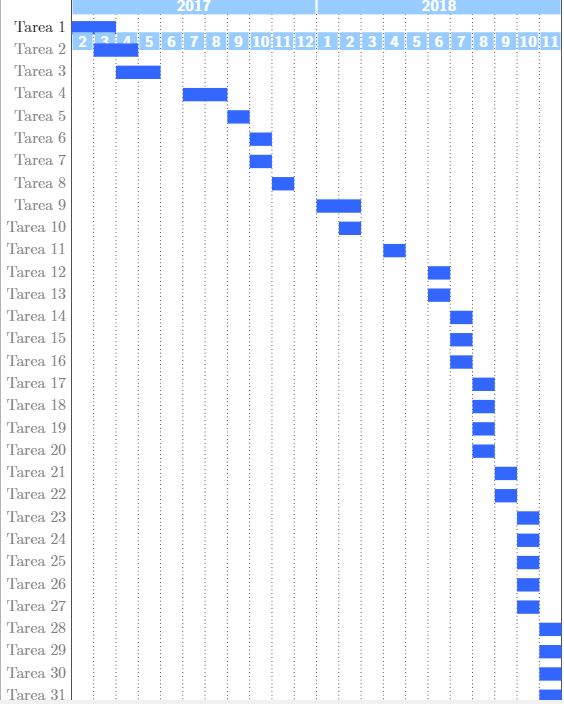
\includegraphics[width=\textwidth]{CronogramaTareas/cronogramaTareas.PNG}
	\caption{Cronograma de tareas.
	\label{fig:CronogramaTareas/cronogramaTareas.PNG}}
\end{figure}

En la figura \ref{fig:CronogramaTareas/cronogramaTareas.PNG} se muestra un cronograma de tareas con las tareas realizadas en este trabajo de fin de grado (TFG) y sus respectivas duraciones.

\section{Descripción de los requerimientos/requisitos}

En la elaboración de este TFG, se ha creado además un programa de ordenador en lenguaje de programación Python. Para ello, se requerían de los siguientes elementos:

Ordenador personal con conectividad Wi-Fi.

Agregar unas variables de entorno en el sistema, explicado previamente en este informe.

Tener instalados los siguientes programas en el sistema:

- ‘IDLE (Python 3.6 64-bit)’, concretamente la versión ‘3.6.4’.

- ‘Git Bash’, versión 2.7.7 para sistemas de 64 bits.

- 'Texmaker 5.0.2.', para realizar este informe o memoria.

\section{Entradas y salidas}

El software requiere de un vídeo cualquiera en formato MP4, de cualquier resolución, y guardado en una ubicación o ruta cualquiera en el disco duro del PC. El vídeo preferentemente será de helióstatos, con el fin de sacar el máximo partido al código ya que este está adaptado para procesar helióstatos.

En el código de ese software, se han utilizado las siguientes variables de entrada:

- \verb|start_time|. Indica el tiempo de ejecución nada más iniciar la ejecución del programa.

- \verb|frame_counter|. Cuenta los fotogramas analizados del vídeo.

- \verb|end_time|. Indica el tiempo de ejecución tras haber procesado un fotograma del vídeo (o tiempo final), y lo mismo para los siguientes, en cuyo caso el tiempo final nunca se reinicia a cero, sino que es acumulado.

- \verb|fps|. Con la fórmula \verb|frame_counter / float(end_time - start_time)|, es decir, usando las variables anteriores, se calcula, para cada fotograma analizado del vídeo, sus fotogramas por segundo.

- \verb|parser|. Permite definir unos parámetros para que cuando se ejecute el programa por consola, se proporcione como parámetros o entradas (y en el siguiente orden) la ruta o directorio del vídeo a leer en el PC, el ancho y el alto mínimos del helióstato para su detección y análisis.

- \verb|args|. Devuelve o carga el parámetro deseado y que fueron especificados por el usuario (explicado previamente): directorio, ancho o alto.

- \verb|camara|. Contenido del vídeo de helióstatos que se irá leyendo, fotograma a fotograma, por el software.

- \verb|grabbed|. Indica si se ha logrado cargar el siguiente fotograma del vídeo de helióstatos, queriendo además decir que dicho vídeo aún no se han analizado todos sus fotogramas y que debe proseguir la ejecución del programa.

- \verb|frame|. Es el contenido del fotograma concreto del vídeo de helióstatos.

- \verb|img|. Es el vídeo de helióstatos convertido a escala de grises.

- \verb|thresh|. Aplicar un umbral para cada fotograma del vídeo de helióstatos, con el fin de determinar en cada píxel, si este es relativamente brillante o no lo es.

- \verb|i|. Para el fotograma del vídeo actual, indica el número de helióstato en análisis: 0 (helióstato 1) ó 1 (helióstato 2).

- \verb|contours|. Todos los contornos o helióstatos detectados, para cada fotograma del vídeo de helióstatos.

- \verb|x, y, w, h|. Referido al contorno en análisis: \verb|xy| son las coordenadas de un punto, \verb|w| es el ancho, y \verb|h| es la altura.

- \verb|area|. Valor del área del contorno o helióstato en análisis.

- \verb|m|. Vector BGR en tres dimensiones que representa dicha información del helióstato en análisis.

- \verb|mB|, \verb|mG|, \verb|mR|. Lo mismo que la variable anterior \verb|m|, pero esta vez separadas en sus distintas componentes BGR.

- \verb|mB2|, \verb|mG2|, \verb|mR2|. Resultados de elevar al cuadrado los valores de las componentes BGR del helióstato.

- \verb|sumB|, \verb|sumG| y \verb|sumR|. Indica la sumatoria acumulativa de todos los píxeles de valor R al cuadrado del helióstato en análisis, y respectivamente para G y B.

- \verb|sumaBGR|. Indica la sumatoria de todos los píxeles de valores R al cuadrado más G al cuadrado más B al cuadrado del helióstato en análisis.

- \verb|heliostato|, \verb|anchoAlto|, \verb|areaTotal|, \verb|sumaBGRparcial|, \verb|sumaBGRtotal|. Variables en forma de arrays que almacenan (y después muestran en consola) los textos, datos y resultados de los helióstatos analizados. Cada array almacena su correspondiente información.\\[20pt]

Las siguientes variables de entrada son completamente personalizables por el usuario, ya que estas son insertables desde la ventana de comandos de Windows al ejecutar el programa:

- \verb|args.directorioVideoHeliostatosCargar|. Parámetro que el programa solicita al usuario para que lo introduzca por consola y que permite indicar el directorio o ruta donde se ubica el vídeo de helióstatos a procesar.

- \verb|args.umbralVideoHeliostatos|. Parámetro que el programa solicita al usuario para que lo introduzca por consola y que permite definir el umbral del vídeo de helióstatos para que, si los píxeles (del helióstato) en análisis de ese vídeo superan ese umbral, sean analizados, y viceversa.

- \verb|args.numeroHeliostatosAnalizar|. Parámetro que el programa solicita al usuario para que lo introduzca por consola y que permite definir el número máximo de helióstatos que serán analizados (si cumplen los requisitos) en cada fotograma del vídeo de helióstatos, ignorando así posibles falsos contornos/helióstatos que suelen ser más pequeños que los helióstatos reales.

- \verb|args.anchoMinimoHeliostato|, \verb|args.altoMinimoHeliostato|. Parámetros que el programa solicita al usuario para que los introduzca por consola y que permiten definir el ancho/alto mínimos que debe tener el helióstato para ser analizado.\\[20pt]

Las siguientes variables no son usadas para este proyecto y se explicarán muy brevemente. No obstante, era necesario declararlas para evitar errores de compilación en el software.

- \verb|ret|. Umbralización de Otsu en el vídeo de helióstatos.

- \verb|im2|. Imagen fuente, procedente del fotograma actual del vídeo de helióstatos.

- \verb|hierarchy|. Método de aproximación del contorno.\\[20pt]

Tras el uso de las variables de entrada anteriores, el software mostrará por pantalla una consola de información y resultados y dos ventanas del vídeo de helióstatos. Ambos elementos se van actualizando en tiempo de ejecución. Los resultados mostrados en consola de los helióstatos son finales, no parciales. En la consola aparece la siguiente información, para cada fotograma del vídeo de helióstatos:

\begin{lstlisting}
Analizando el helióstato verde y/o rojo.
Ancho y alto del helióstato en píxeles.
Área del helióstato en píxeles.
Sumatorias acumulativas de los valores BGR al cuadrado (cada componente por separado) de todos los píxeles del helióstato en análisis.
Suma total (o unificación) de esas tres componentes BGR entre sí.
Fotogramas por segundo del vídeo.
\end{lstlisting}

Ejemplos gráficos (figuras \ref{fig:CapturasEntradasYSalidas/Captura(2).PNG} y \ref{fig:CapturasEntradasYSalidas/Captura(3).PNG}):

\begin{figure}[h!]
  	\centering
	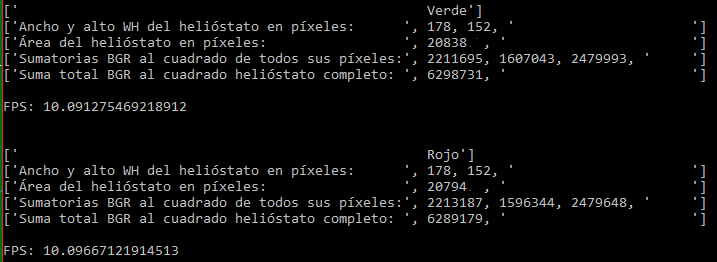
\includegraphics[width=\textwidth]{CapturasEntradasYSalidas/Captura(2).PNG}
	\caption{Resultados por consola al analizar el helióstato verde y rojo, aparecidos en distintos fotogramas del vídeo.
	\label{fig:CapturasEntradasYSalidas/Captura(2).PNG}}
\end{figure}

\begin{figure}[h!]
  	\centering
	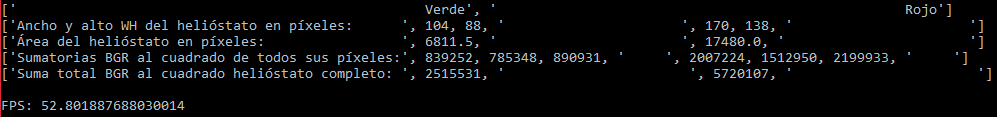
\includegraphics[width=\textwidth]{CapturasEntradasYSalidas/Captura(3).PNG}
	\caption{Resultados por consola al analizar el helióstato verde y rojo, aparecidos en el mismo fotograma del vídeo.
	\label{fig:CapturasEntradasYSalidas/Captura(3).PNG}}
\end{figure}

En las ventanas del vídeo de helióstatos, en una de ellas aparece el vídeo umbralizado, con el fin de detectar lo que son contornos (helióstatos) e ignorar los que no lo sean, así como los falsos contornos. Y en la otra ventana, aparece el vídeo original. En esta última, cuando se detecten helióstatos de un tamaño (ancho y alto) determinados (deseados por el usuario en los parámetros que él mismo proporcionó al ejecutar el programa), se reencuadrará con un cuadrado o rectángulo verde o rojo y se analizará por el software. El rectángulo en general será de color verde si solo se muestra un helióstato (o dos helióstatos rozándose entre sí, tratados como si fueran uno solo) en el fotograma actual del vídeo, pero si en dicho fotograma se muestran dos helióstatos (y separados entre sí), el rectángulo para el helióstato secundario será rojo. Esto permitirá diferenciar bien los helióstatos, y saber qué información mostrada en consola le corresponde a cada helióstato.

Ejemplo gráfico (figura \ref{fig:CapturasEntradasYSalidas/unnamed(1).png}):

\begin{figure}[h!]
  	\centering
	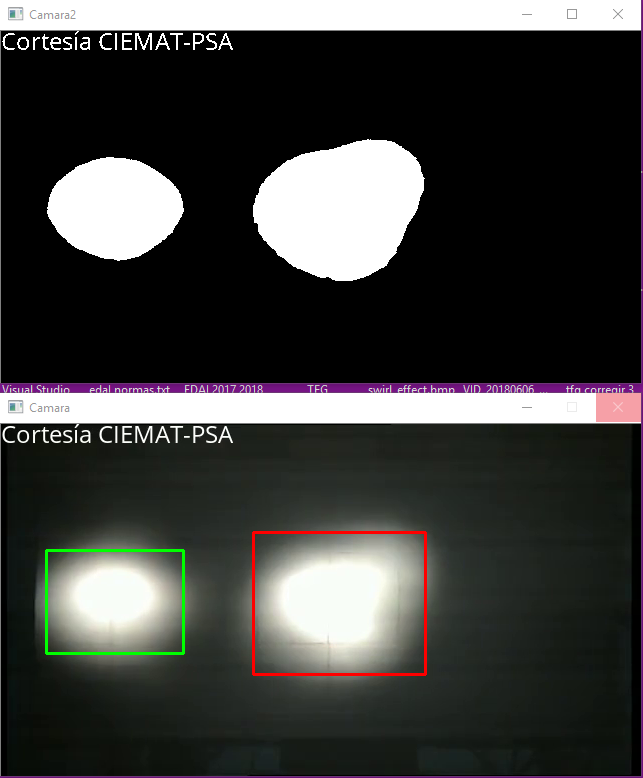
\includegraphics[width=\textwidth]{CapturasEntradasYSalidas/unnamed(1).png}
	\caption{El software detecta, analiza y reencuadra en el vídeo los helióstatos detectados, y en distintos colores para su diferenciación.
	\label{fig:CapturasEntradasYSalidas/unnamed(1).png}}
\end{figure}

\section{Análisis de los recursos consumidos}

A continuación, se mostrarán y explicarán los resultados del uso de la CPU y del consumo de la memoria RAM en el PC, en el administrador de tareas de Windows 10, durante la ejecución del software en distintos periodos de tiempo. También se medirán los fotogramas por segundo (FPS) actuales del vídeo.

\subsection{Cargando el vídeo 'variosHeliostatos.mp4'}

Se inicia la ejecución del software desde la terminal de Windows, estando en el directorio que contiene dicho software a ejecutar, y usando el comando \verb|estimacion_potencia.py Videos/varios_heliostatos.mp4 50 50 127 2|.

\begin{figure}[h!]
  	\centering
	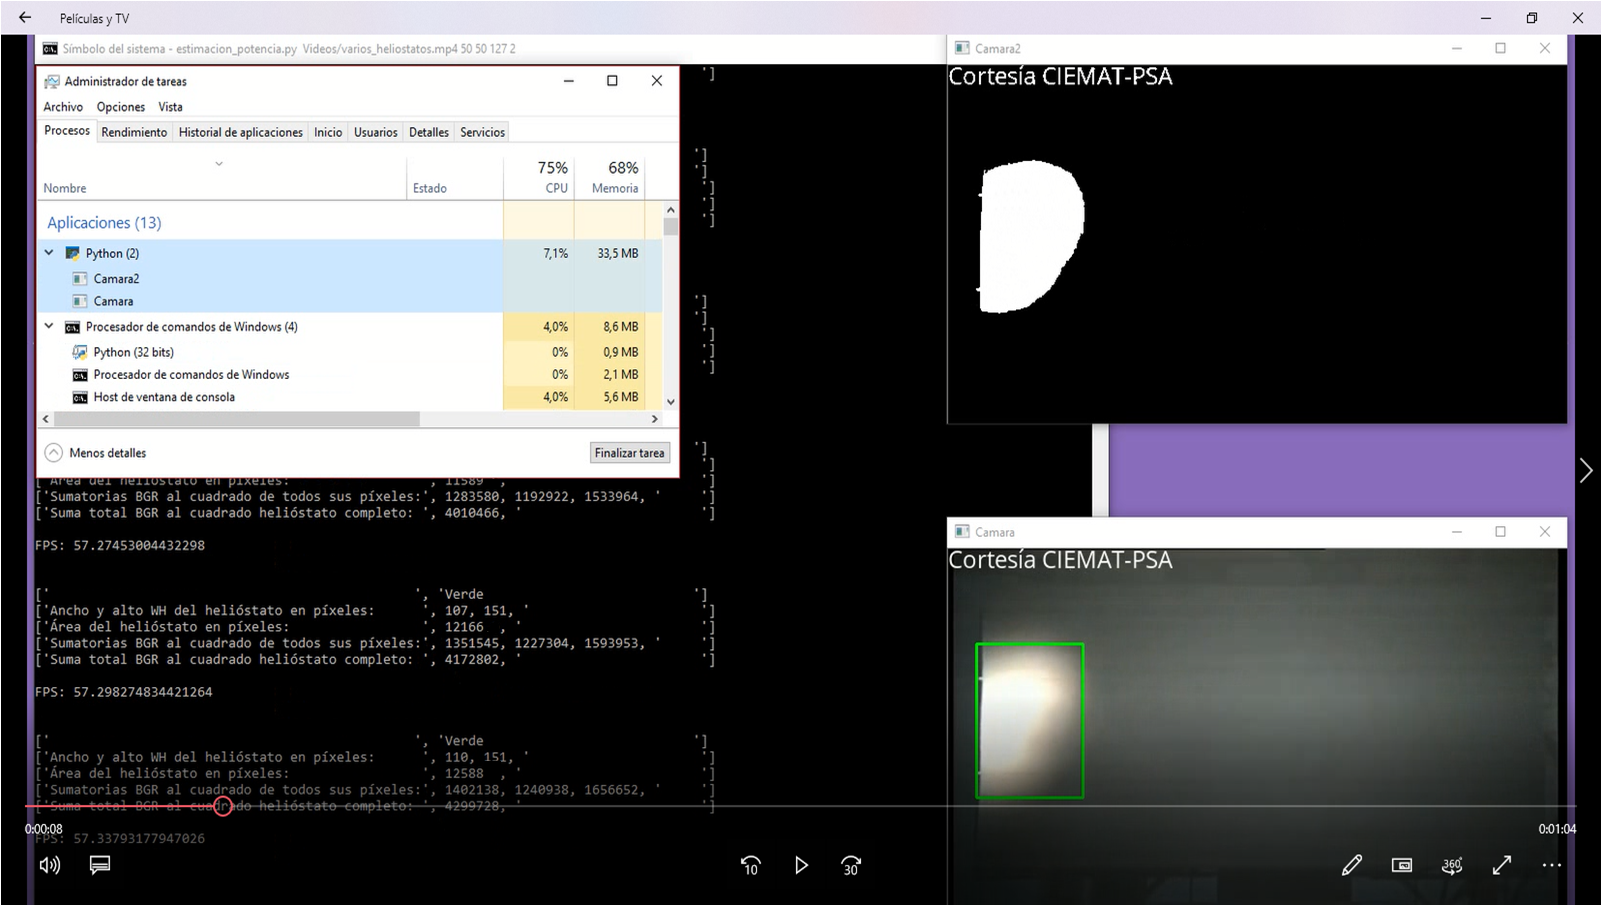
\includegraphics[width=\textwidth]{CapturasRendimientoSoftware1/Imagen1.png}
	\caption{Instante de tiempo 1 de la ejecución del software para el vídeo 'varios\_heliostatos.mp4'.
	\label{fig:CapturasRendimientoSoftware1/Imagen1.png}}
\end{figure}

Figura \ref{fig:CapturasRendimientoSoftware1/Imagen1.png}. Al iniciar la ejecución del software, cuando está entrando el primer helióstato desde el lado izquierdo en el vídeo y aún no se muestra en su totalidad, Python consume un 7,1\% de CPU y 33,5 MB de memoria RAM, mientras que la terminal de Windows consume un 4\% de CPU y 8,6 MB de memoria RAM. Los FPS son de 57,27.\\[20pt]

\begin{figure}[h!]
  	\centering
	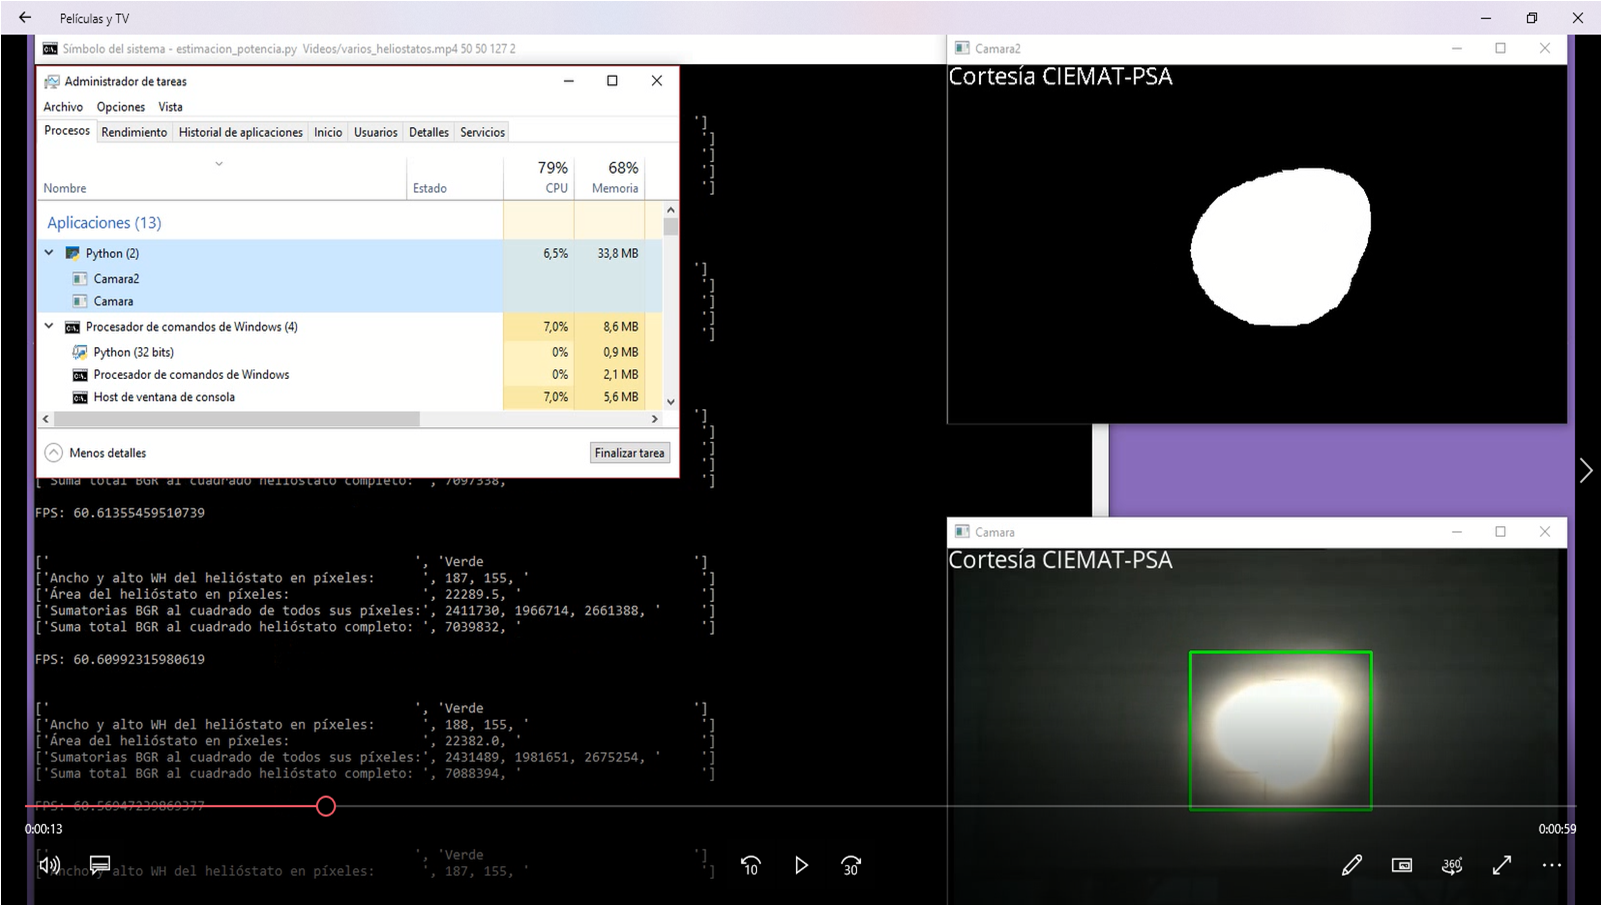
\includegraphics[width=\textwidth]{CapturasRendimientoSoftware1/Imagen2.png}
	\caption{Instante de tiempo 2 de la ejecución del software para el vídeo 'varios\_heliostatos.mp4'.
	\label{fig:CapturasRendimientoSoftware1/Imagen2.png}}
\end{figure}

Figura \ref{fig:CapturasRendimientoSoftware1/Imagen2.png}. Cuando el primer helióstato ya ha llegado al centro del vídeo, Python consume un 6,5\% de CPU y 33,8 MB de memoria RAM, mientras que la terminal de Windows consume un 7\% de CPU y 8,6 MB de memoria RAM. Los FPS son de 60,61.\\[20pt]

\begin{figure}[h!]
  	\centering
	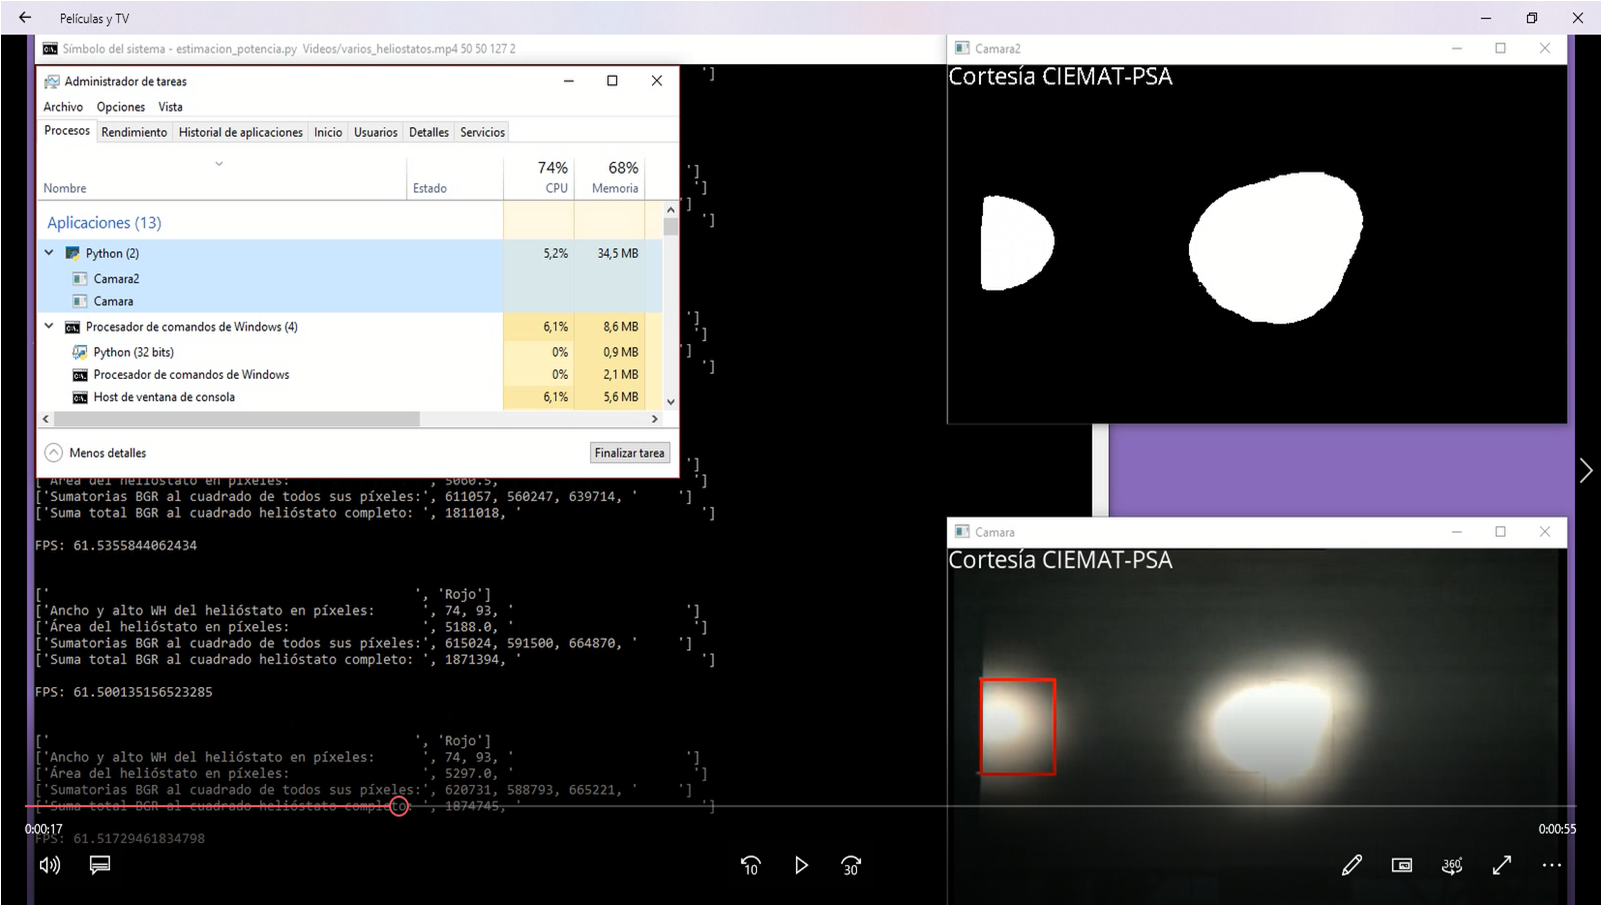
\includegraphics[width=\textwidth]{CapturasRendimientoSoftware1/Imagen3.png}
	\caption{Instante de tiempo 3 de la ejecución del software para el vídeo 'varios\_heliostatos.mp4'.
	\label{fig:CapturasRendimientoSoftware1/Imagen3.png}}
\end{figure}

Figura \ref{fig:CapturasRendimientoSoftware1/Imagen3.png}. Cuando está entrando desde la izquierda del vídeo el segundo helióstato, Python consume un 5,2\% de CPU y 34,5 MB de memoria RAM, mientras que la terminal de Windows consume un 6,1\% de CPU y 8,6 MB de memoria RAM. Los FPS son de 61,53.\\[20pt]

\begin{figure}[h!]
  	\centering
	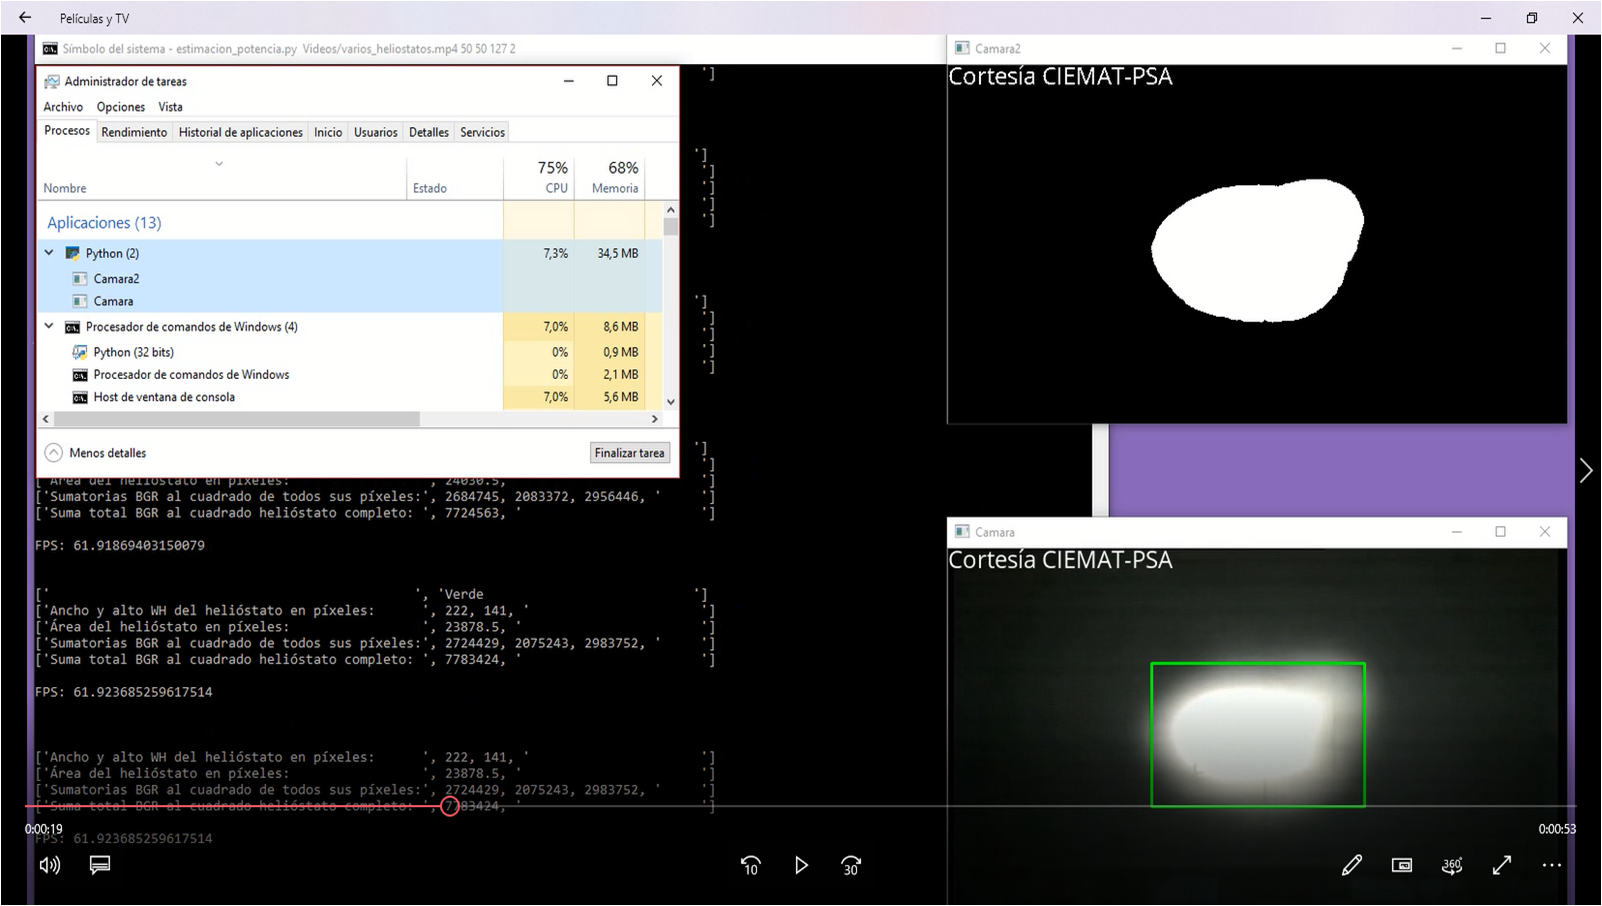
\includegraphics[width=\textwidth]{CapturasRendimientoSoftware1/Imagen4.png}
	\caption{Instante de tiempo 4 de la ejecución del software para el vídeo 'varios\_heliostatos.mp4'.
	\label{fig:CapturasRendimientoSoftware1/Imagen4.png}}
\end{figure}

Figura \ref{fig:CapturasRendimientoSoftware1/Imagen4.png}. Cuando el segundo helióstato prácticamente se ha fusionado con el helióstato permanecido en el centro del vídeo, Python consume un 7,3\% de CPU y 34,5 MB de memoria RAM, mientras que la terminal de Windows consume un 7\% de CPU y 8,6 MB de memoria RAM. Los FPS son de 61,91.\\[20pt]

\begin{figure}[h!]
  	\centering
	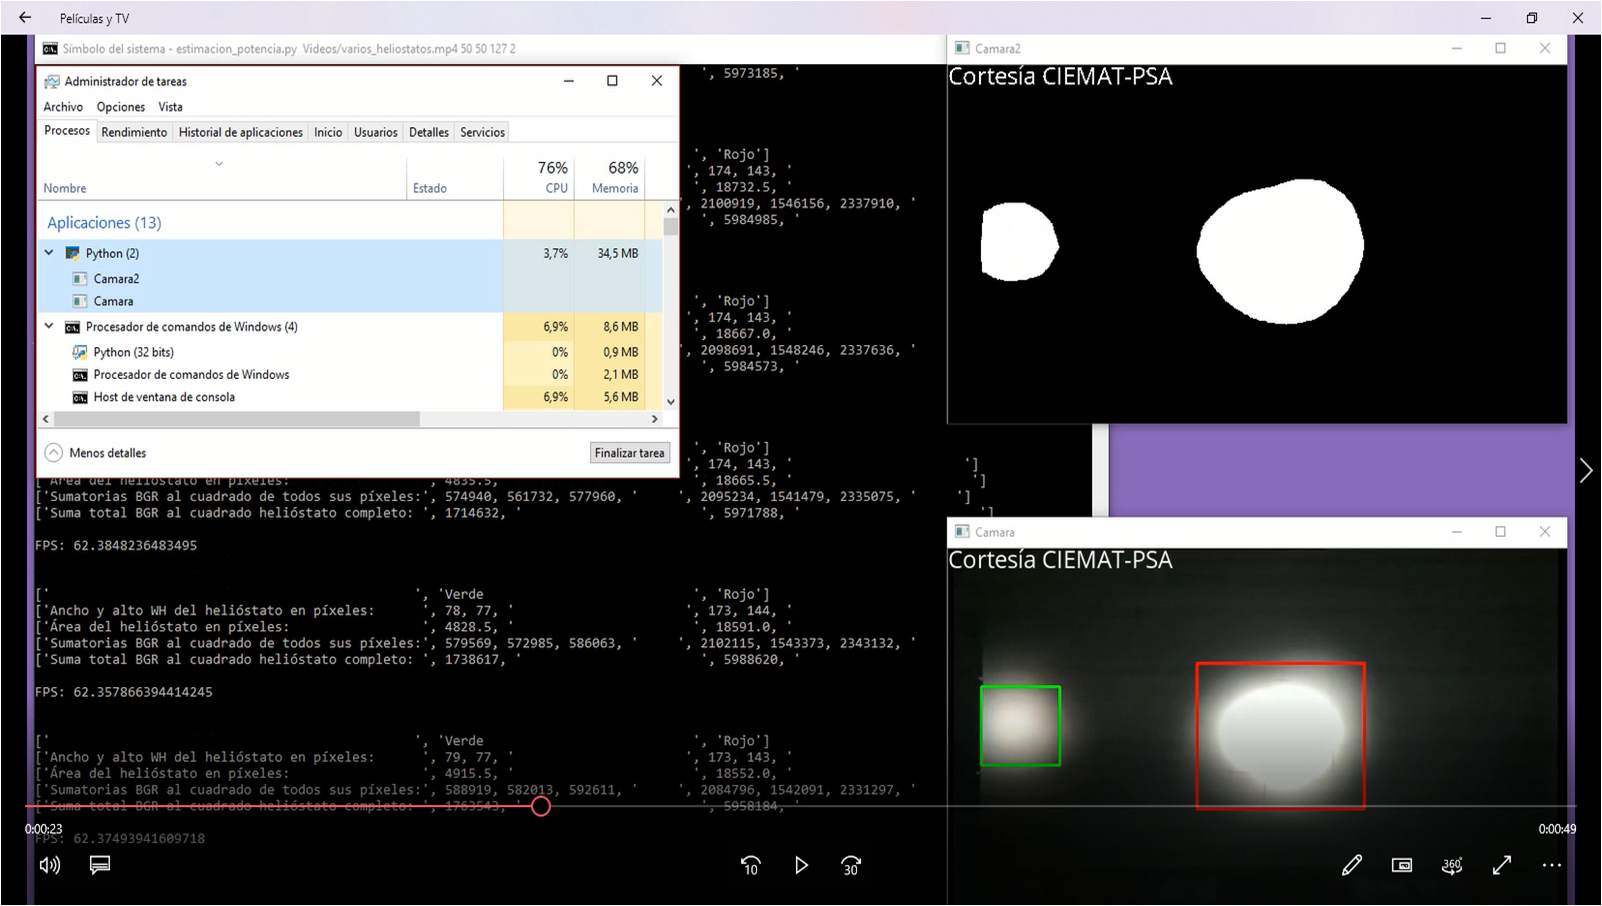
\includegraphics[width=\textwidth]{CapturasRendimientoSoftware1/Imagen5.png}
	\caption{Instante de tiempo 5 de la ejecución del software para el vídeo 'varios\_heliostatos.mp4'.
	\label{fig:CapturasRendimientoSoftware1/Imagen5.png}}
\end{figure}

Figura \ref{fig:CapturasRendimientoSoftware1/Imagen5.png}. Cuando está entrando desde la izquierda del vídeo el tercer helióstato, Python consume un 3,7\% de CPU y 34,5 MB de memoria RAM, mientras que la terminal de Windows consume un 6,9\% de CPU y 8,6 MB de memoria RAM. Los FPS son de 62,38.\\[20pt]

\begin{figure}[h!]
  	\centering
	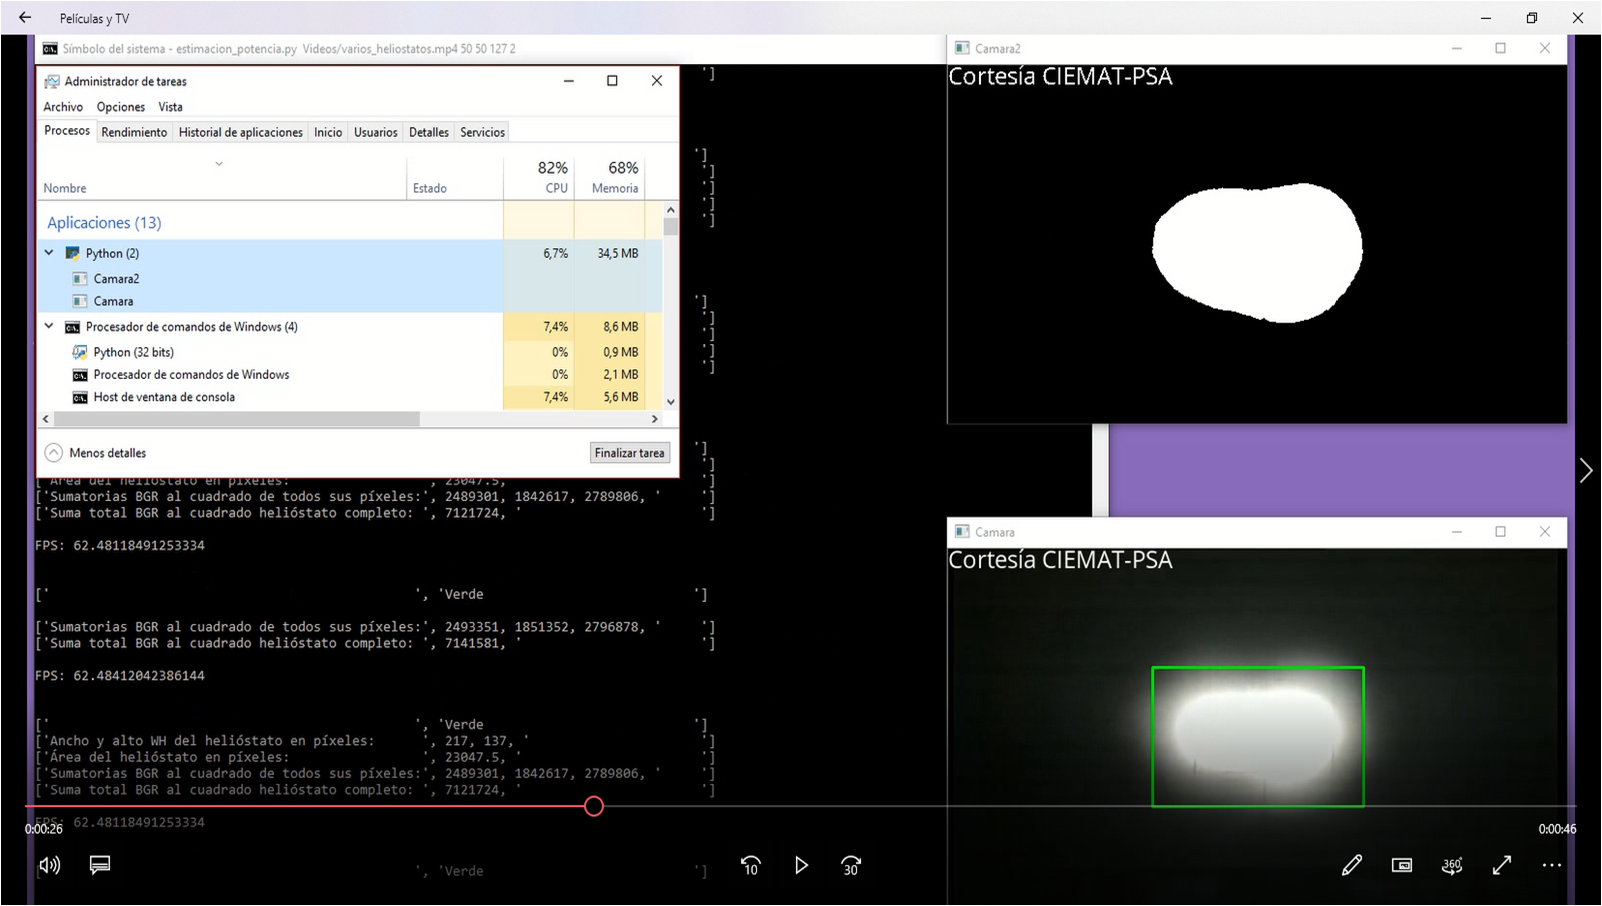
\includegraphics[width=\textwidth]{CapturasRendimientoSoftware1/Imagen6.png}
	\caption{Instante de tiempo 6 de la ejecución del software para el vídeo 'varios\_heliostatos.mp4'.
	\label{fig:CapturasRendimientoSoftware1/Imagen6.png}}
\end{figure}

Figura \ref{fig:CapturasRendimientoSoftware1/Imagen6.png}. Cuando el tercer helióstato prácticamente se ha fusionado con el helióstato permanecido en el centro del vídeo, Python consume un 6,7\% de CPU y 34,5 MB de memoria RAM, mientras que la terminal de Windows consume un 7,4\% de CPU y 8,6 MB de memoria RAM. Los FPS son de 62,48.\\[20pt]

\begin{figure}[h!]
  	\centering
	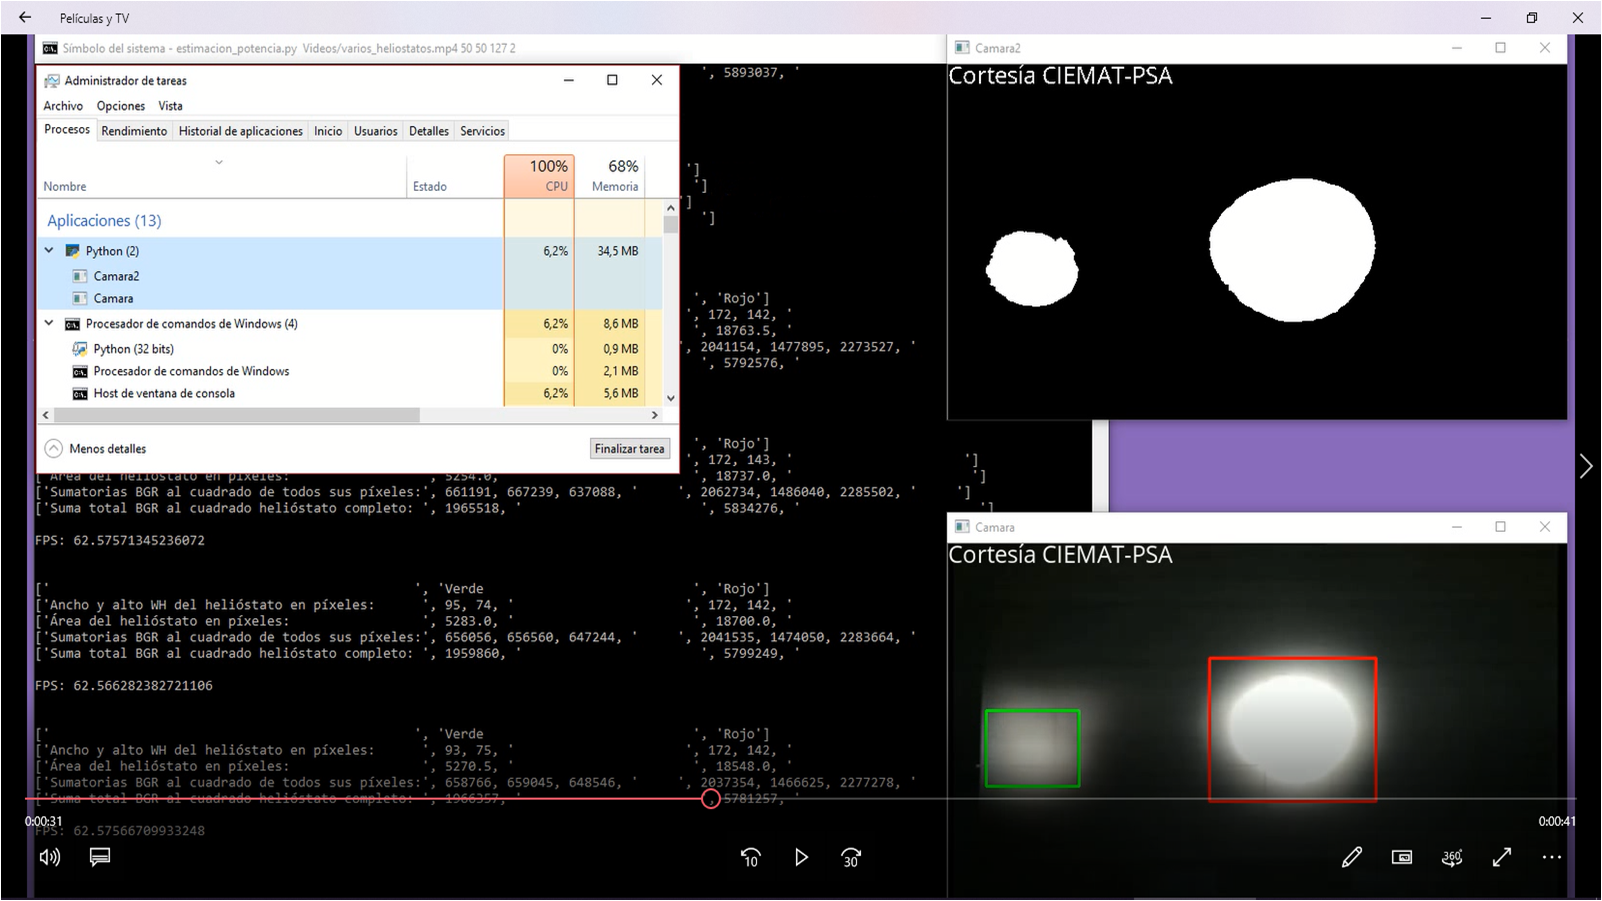
\includegraphics[width=\textwidth]{CapturasRendimientoSoftware1/Imagen7.png}
	\caption{Instante de tiempo 7 de la ejecución del software para el vídeo 'varios\_heliostatos.mp4'.
	\label{fig:CapturasRendimientoSoftware1/Imagen7.png}}
\end{figure}

Figura \ref{fig:CapturasRendimientoSoftware1/Imagen7.png}. Cuando está entrando desde la izquierda del vídeo el cuarto y último helióstato, Python consume un 6,2\% de CPU y 34,5 MB de memoria RAM, mientras que la terminal de Windows consume un 6,2\% de CPU y 8,6 MB de memoria RAM. Los FPS son de 62,57.\\[20pt]

\begin{figure}[h!]
  	\centering
	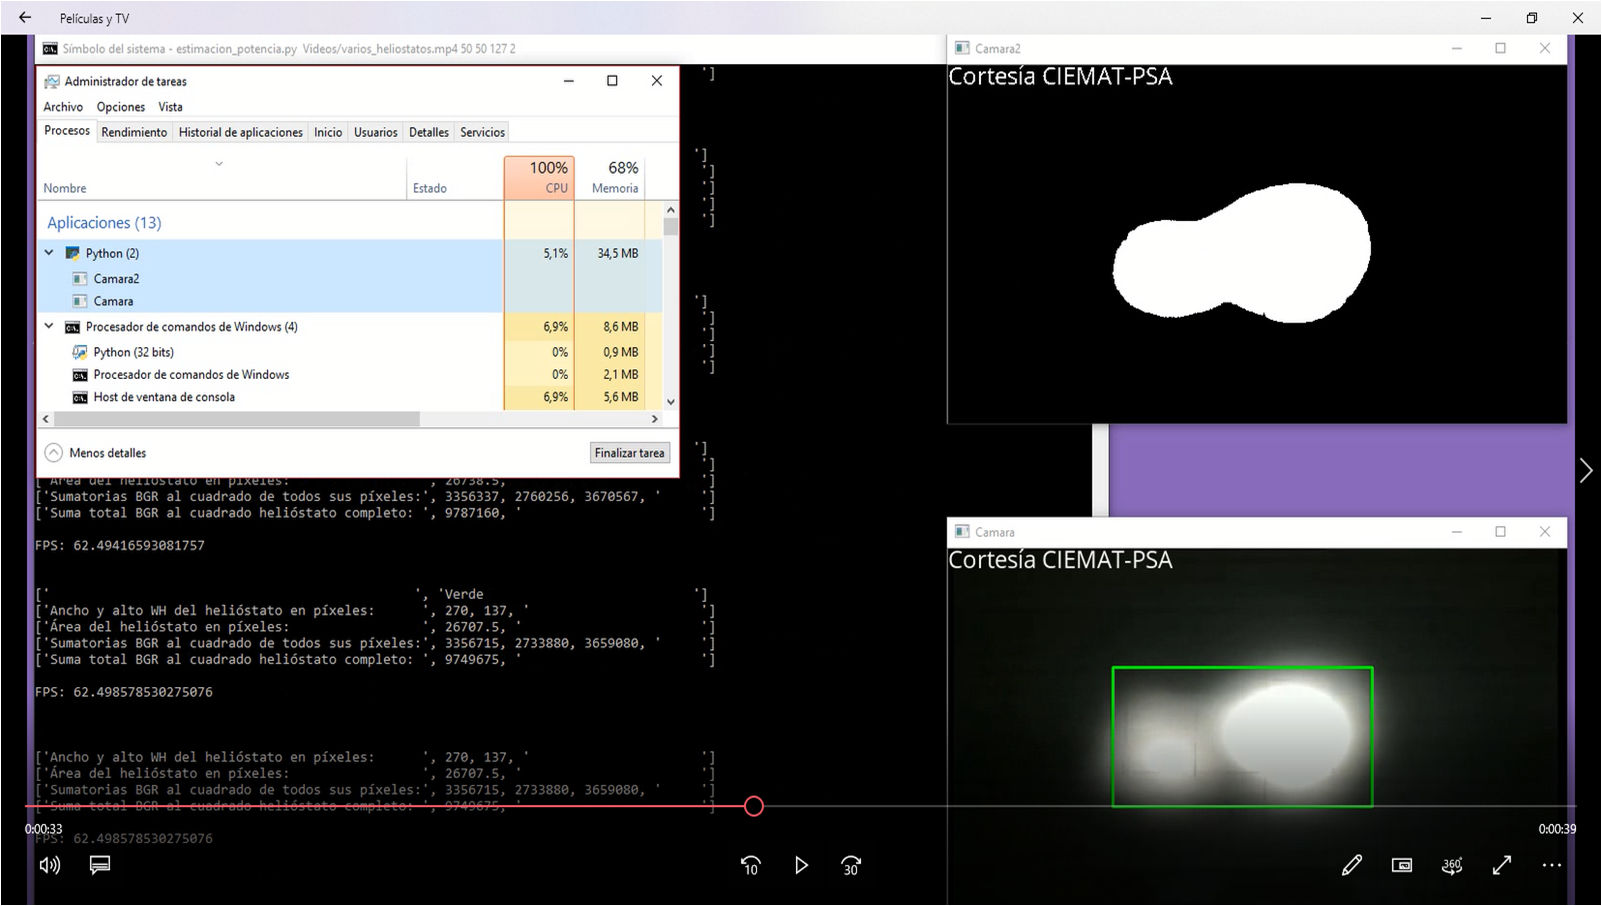
\includegraphics[width=\textwidth]{CapturasRendimientoSoftware1/Imagen8.png}
	\caption{Instante de tiempo 8 de la ejecución del software para el vídeo 'varios\_heliostatos.mp4'.
	\label{fig:CapturasRendimientoSoftware1/Imagen8.png}}
\end{figure}

Figura \ref{fig:CapturasRendimientoSoftware1/Imagen8.png}. Cuando el cuarto helióstato comienza a iniciar la fusión con el helióstato permanecido en el centro del vídeo, Python consume un 5,1\% de CPU y 34,5 MB de memoria RAM, mientras que la terminal de Windows consume un 6,9\% de CPU y 8,6 MB de memoria RAM. Los FPS son de 62,49.\\[20pt]

\begin{figure}[h!]
  	\centering
	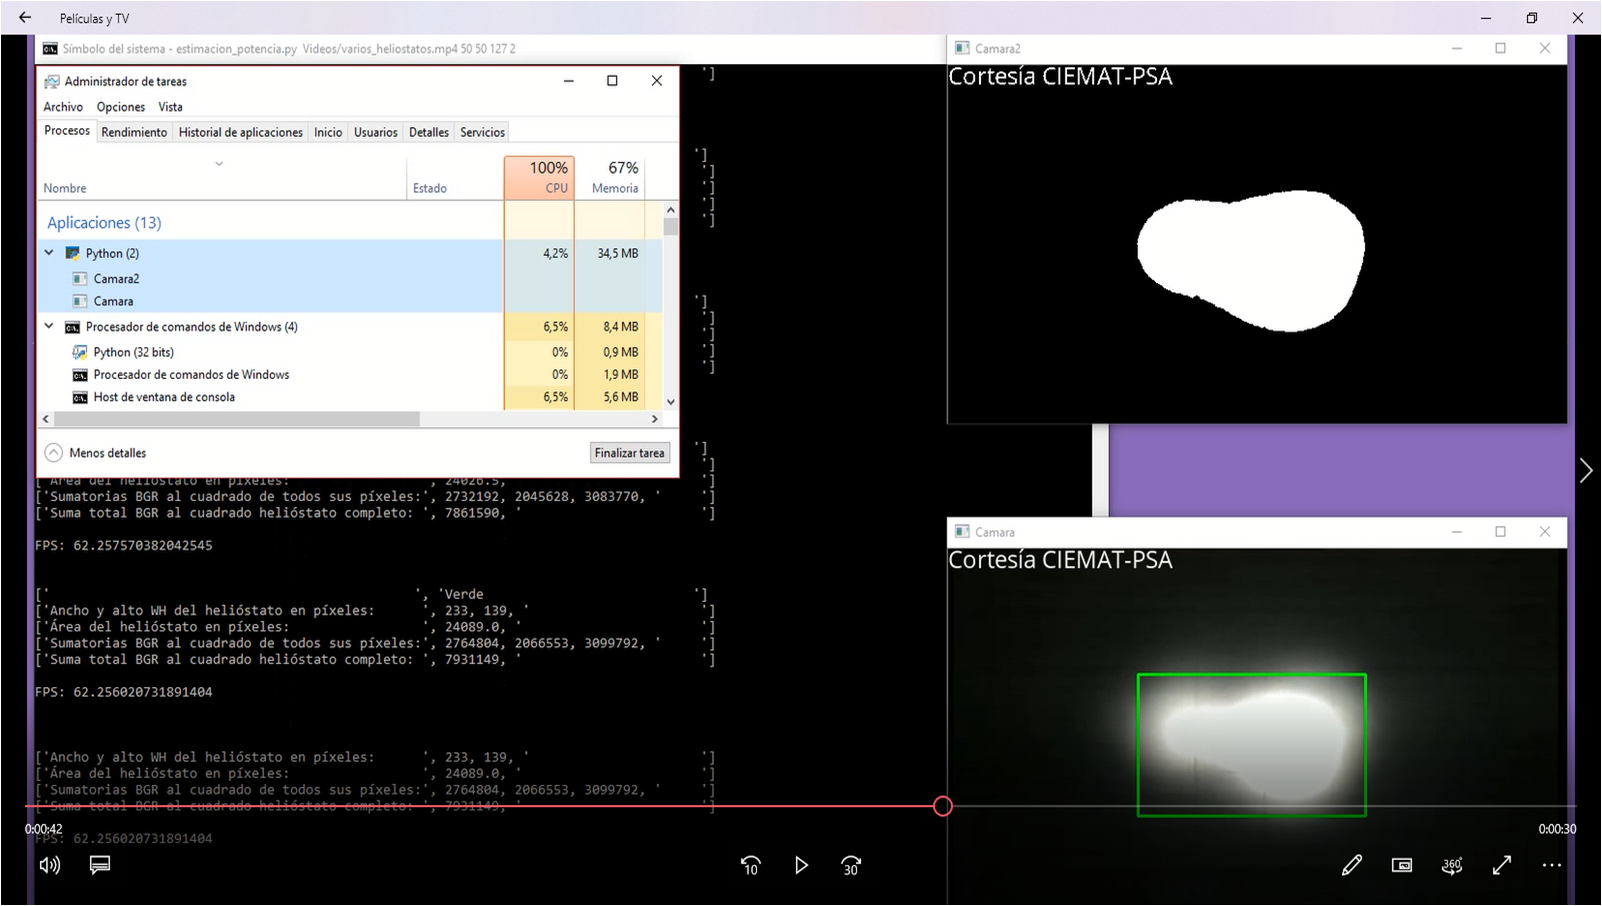
\includegraphics[width=\textwidth]{CapturasRendimientoSoftware1/Imagen9.png}
	\caption{Instante de tiempo 9 de la ejecución del software para el vídeo 'varios\_heliostatos.mp4'.
	\label{fig:CapturasRendimientoSoftware1/Imagen9.png}}
\end{figure}

Figura \ref{fig:CapturasRendimientoSoftware1/Imagen9.png}. Cuando uno de los helióstatos fusionados con el helióstato del centro del vídeo trata de salir del mismo (todavía no se ha completado este procedimiento). Python consume un 4,2\% de CPU y 34,5 MB de memoria RAM, mientras que la terminal de Windows consume un 6,5\% de CPU y 8,4 MB de memoria RAM. Los FPS son de 62,25.\\[20pt]

\begin{figure}[h!]
  	\centering
	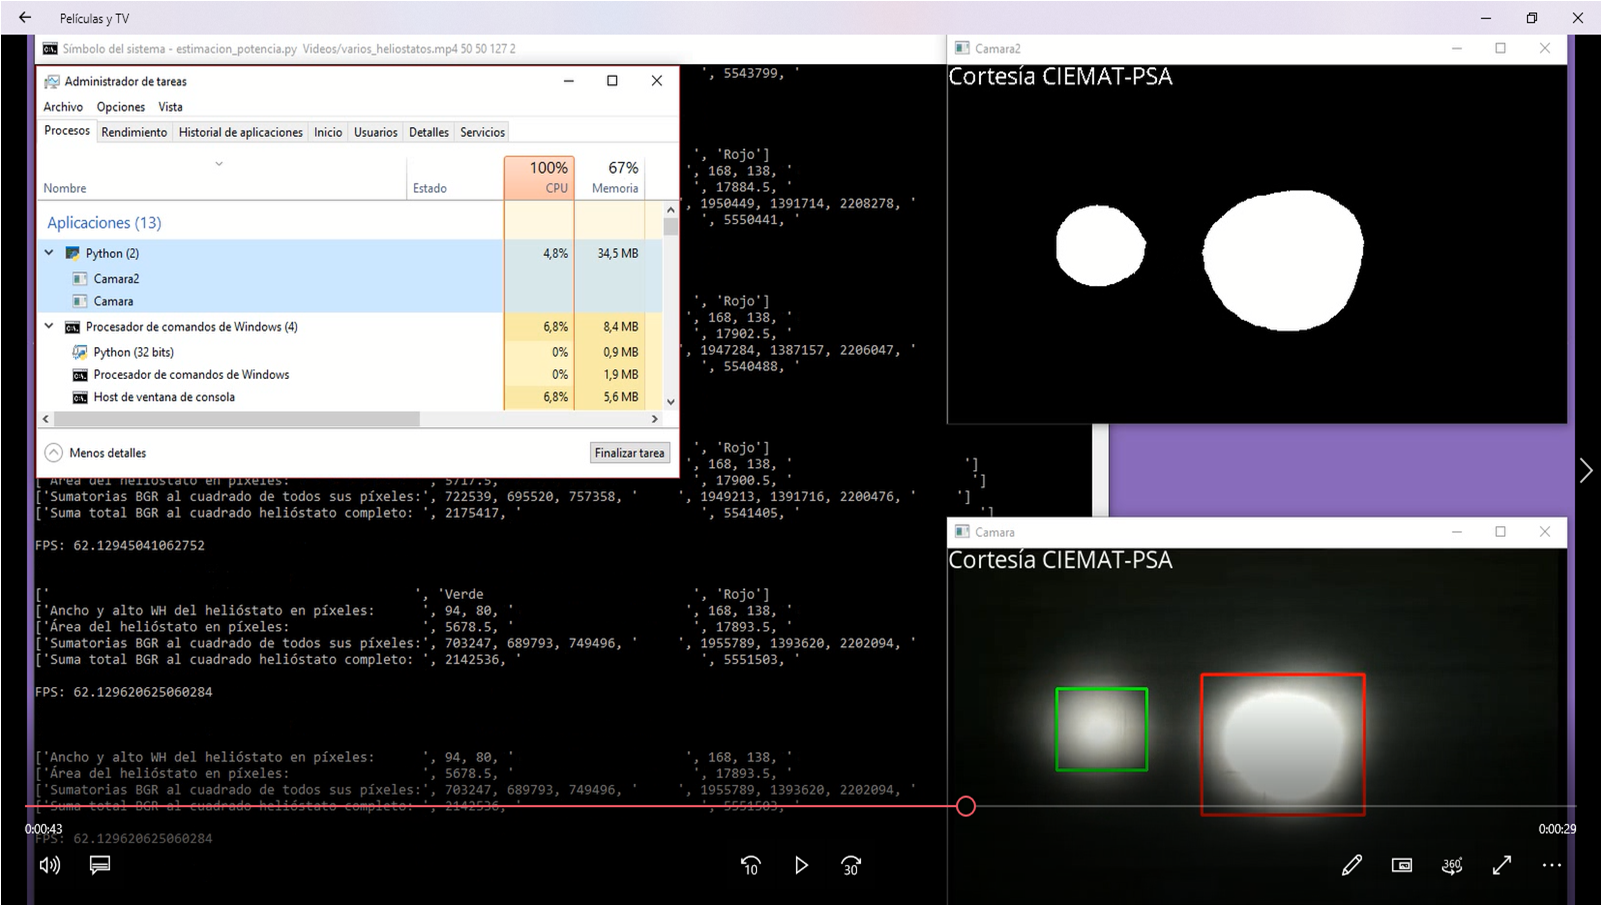
\includegraphics[width=\textwidth]{CapturasRendimientoSoftware1/Imagen10.png}
	\caption{Instante de tiempo 10 de la ejecución del software para el vídeo 'varios\_heliostatos.mp4'.
	\label{fig:CapturasRendimientoSoftware1/Imagen10.png}}
\end{figure}

Figura \ref{fig:CapturasRendimientoSoftware1/Imagen10.png}. Cuando el helióstato ya se ha separado del helióstato central del vídeo, Python consume un 4,8\% de CPU y 34,5 MB de memoria RAM, mientras que la terminal de Windows consume un 6,8\% de CPU y 8,4 MB de memoria RAM. Los FPS son de 62,12.\\[20pt]

\begin{figure}[h!]
  	\centering
	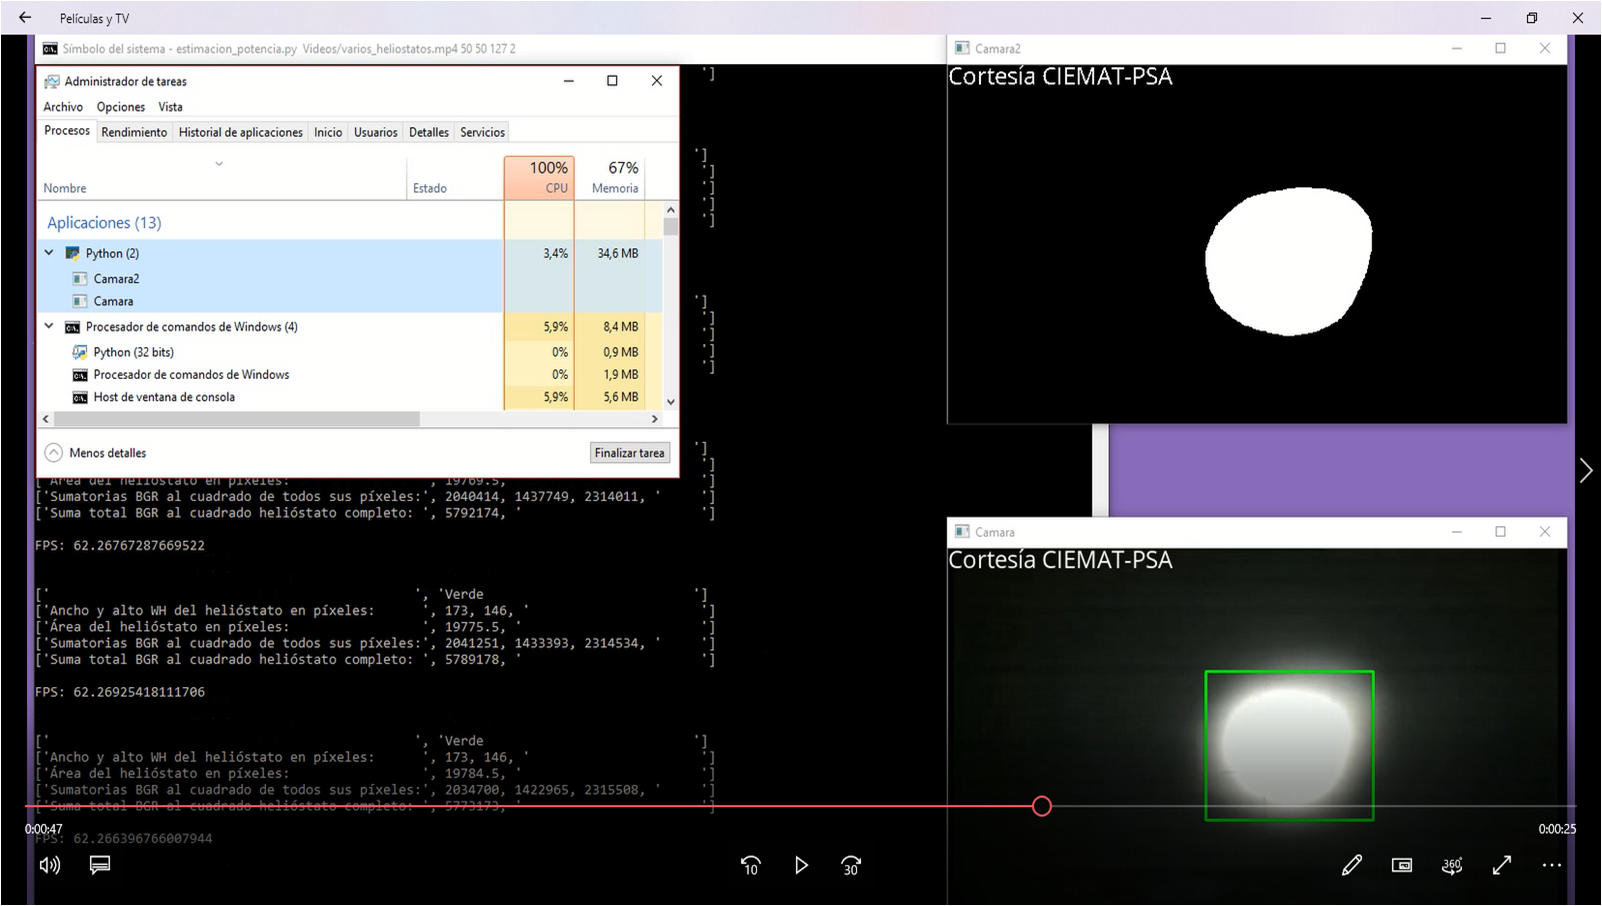
\includegraphics[width=\textwidth]{CapturasRendimientoSoftware1/Imagen11.png}
	\caption{Instante de tiempo 11 de la ejecución del software para el vídeo 'varios\_heliostatos.mp4'.
	\label{fig:CapturasRendimientoSoftware1/Imagen11.png}}
\end{figure}

Figura \ref{fig:CapturasRendimientoSoftware1/Imagen11.png}. Cuando únicamente permanece el helióstato central del vídeo (el otro helióstato ya se ha ido a la izquierda del vídeo), Python consume un 3,4\% de CPU y 34,6 MB de memoria RAM, mientras que la terminal de Windows consume un 5,9\% de CPU y 8,4 MB de memoria RAM. Los FPS son de 62,26.\\[20pt]

\begin{figure}[h!]
  	\centering
	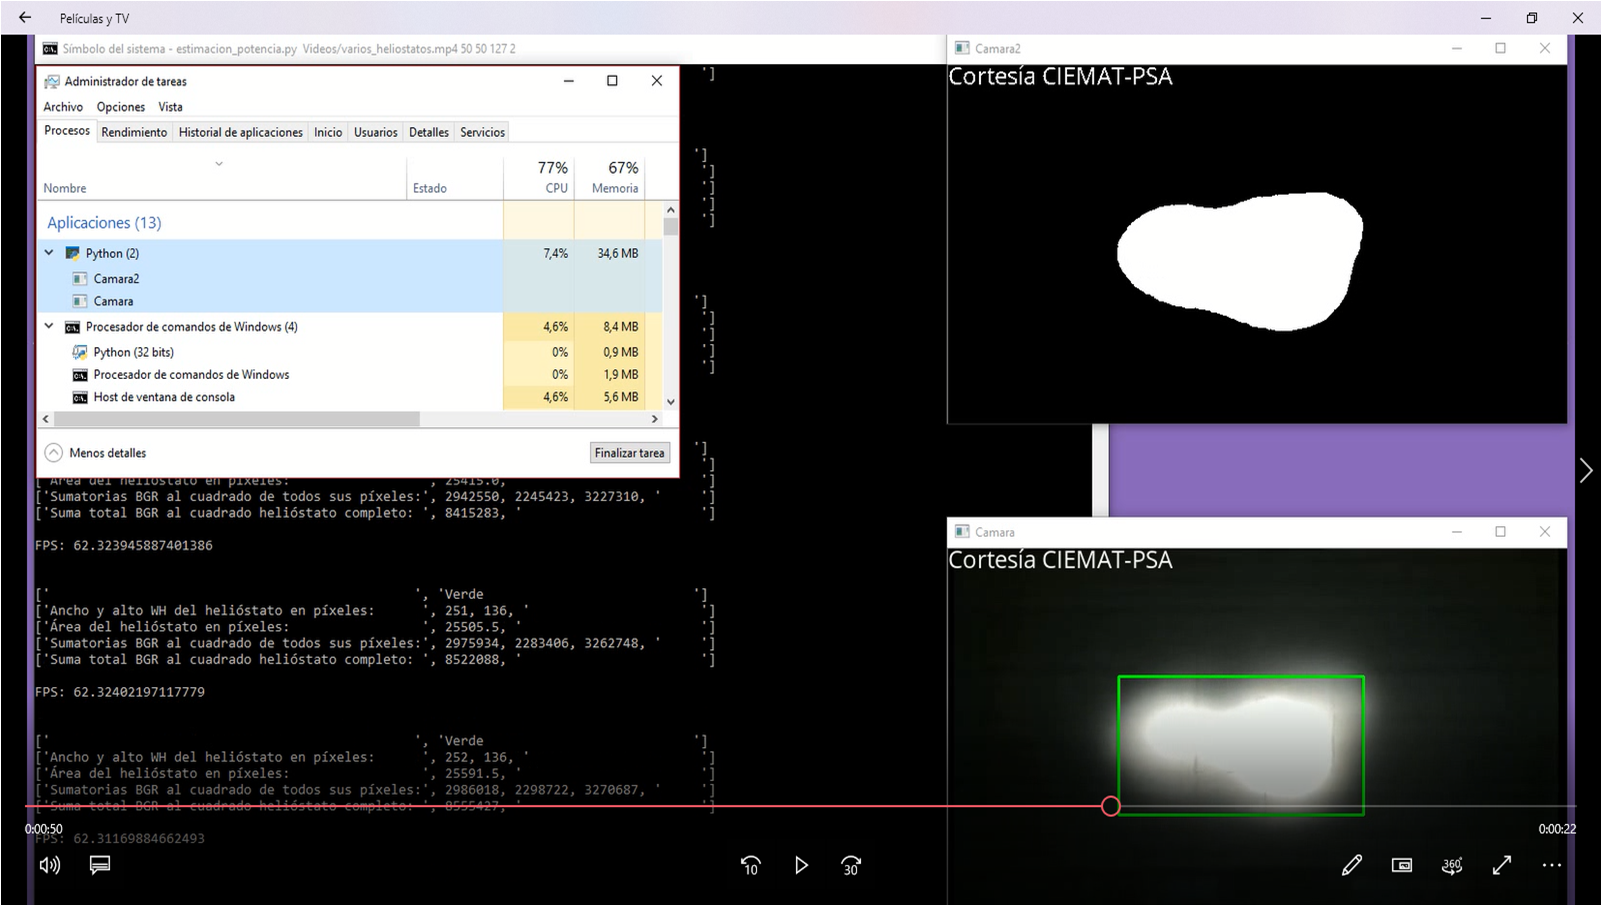
\includegraphics[width=\textwidth]{CapturasRendimientoSoftware1/Imagen12.png}
	\caption{Instante de tiempo 12 de la ejecución del software para el vídeo 'varios\_heliostatos.mp4'.
	\label{fig:CapturasRendimientoSoftware1/Imagen12.png}}
\end{figure}

Figura \ref{fig:CapturasRendimientoSoftware1/Imagen12.png}. Cuando otro de los helióstatos fusionados con el helióstato del centro del vídeo trata de salir del mismo (todavía no se ha completado este procedimiento). Python consume un 7,4\% de CPU y 34,6 MB de memoria RAM, mientras que la terminal de Windows consume un 4,6\% de CPU y 8,4 MB de memoria RAM. Los FPS son de 62,32.\\[20pt]

\begin{figure}[h!]
  	\centering
	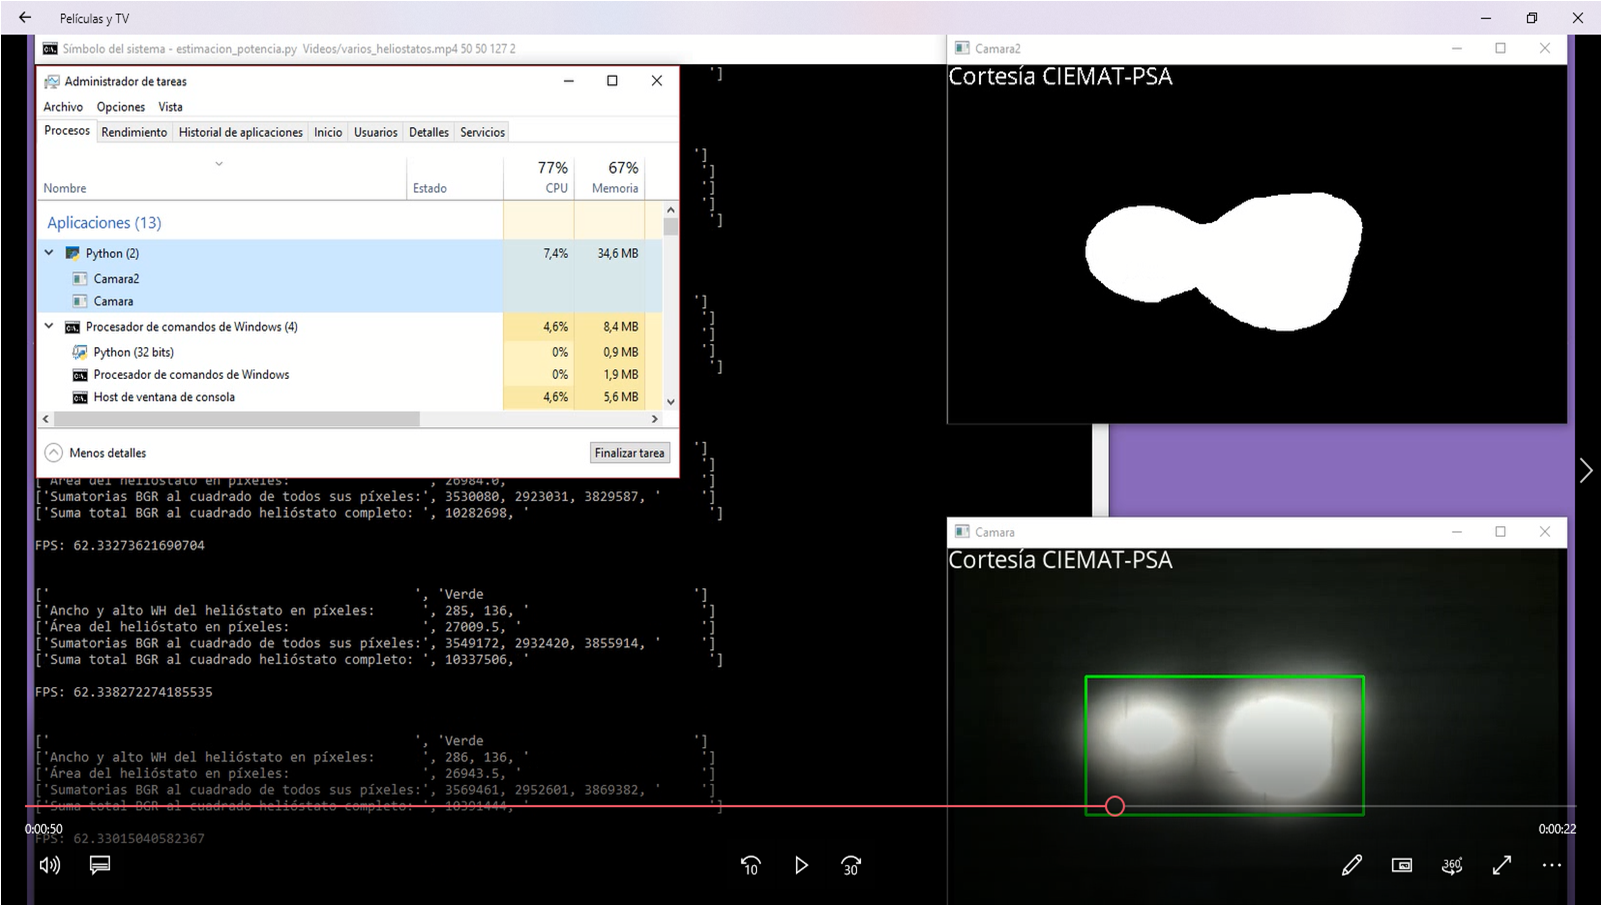
\includegraphics[width=\textwidth]{CapturasRendimientoSoftware1/Imagen13.png}
	\caption{Instante de tiempo 13 de la ejecución del software para el vídeo 'varios\_heliostatos.mp4'.
	\label{fig:CapturasRendimientoSoftware1/Imagen13.png}}
\end{figure}

Figura \ref{fig:CapturasRendimientoSoftware1/Imagen13.png}. Cuando los dos helióstatos están a punto de separarse entre sí. Python consume un 7,4\% de CPU y 34,6 MB de memoria RAM, mientras que la terminal de Windows consume un 4,6\% de CPU y 8,4 MB de memoria RAM. Los FPS son de 62,33.\\[20pt]

\begin{figure}[h!]
  	\centering
	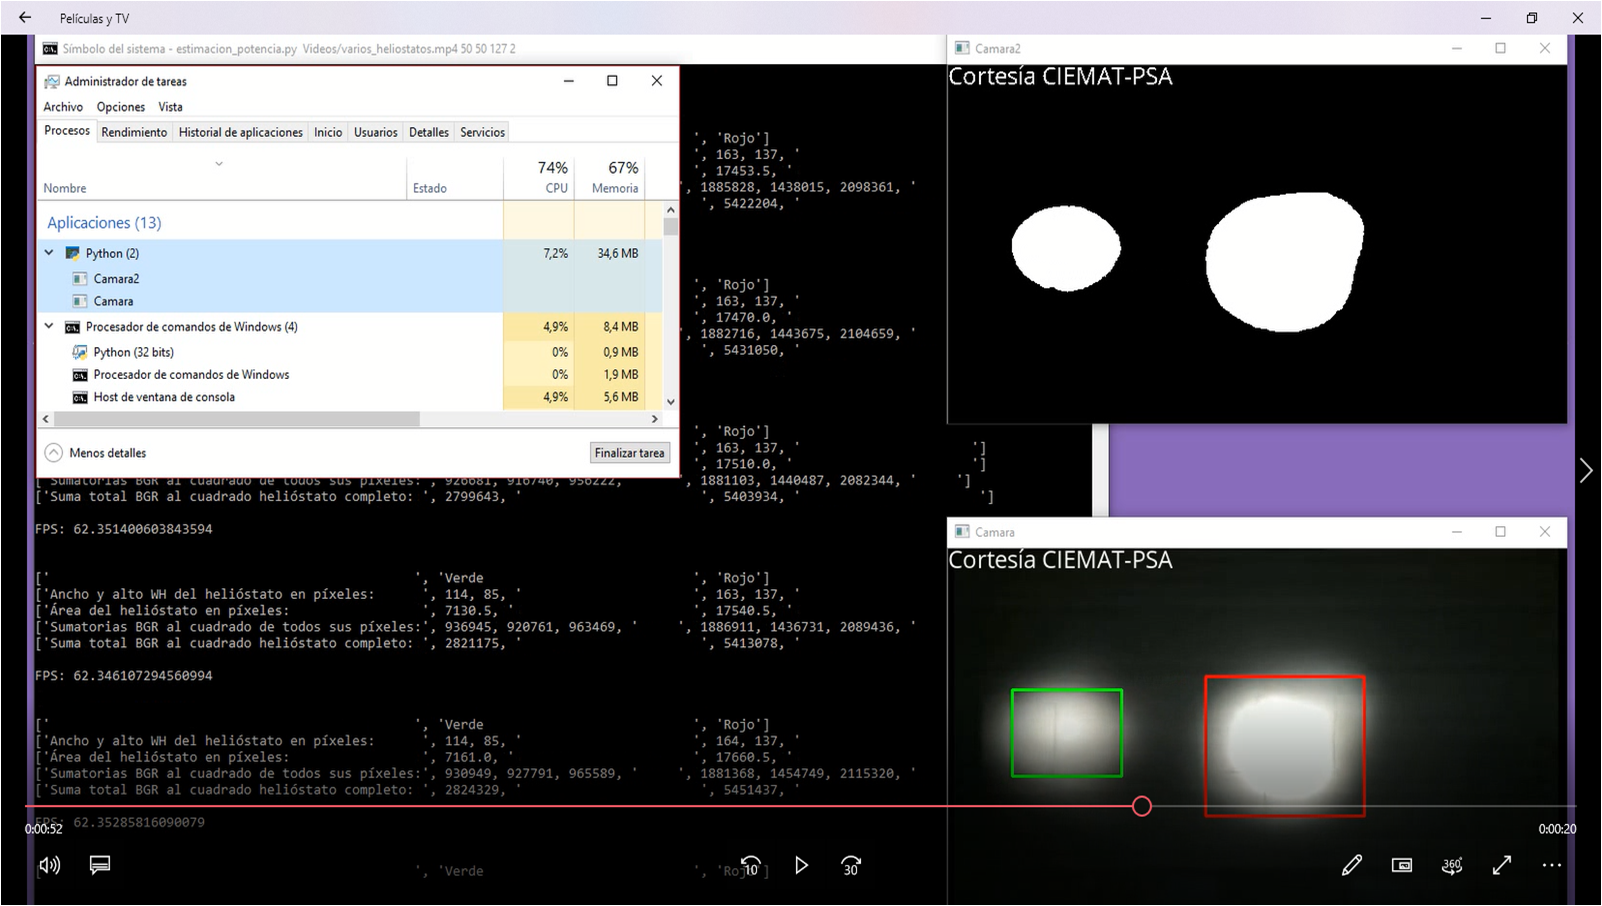
\includegraphics[width=\textwidth]{CapturasRendimientoSoftware1/Imagen14.png}
	\caption{Instante de tiempo 14 de la ejecución del software para el vídeo 'varios\_heliostatos.mp4'.
	\label{fig:CapturasRendimientoSoftware1/Imagen14.png}}
\end{figure}

Figura \ref{fig:CapturasRendimientoSoftware1/Imagen14.png}. Cuando ambos helióstatos ya se han separado entre sí, Python consume un 7,2\% de CPU y 34,6 MB de memoria RAM, mientras que la terminal de Windows consume un 4,9\% de CPU y 8,4 MB de memoria RAM. Los FPS son de 62,35.\\[20pt]

\begin{figure}[h!]
  	\centering
	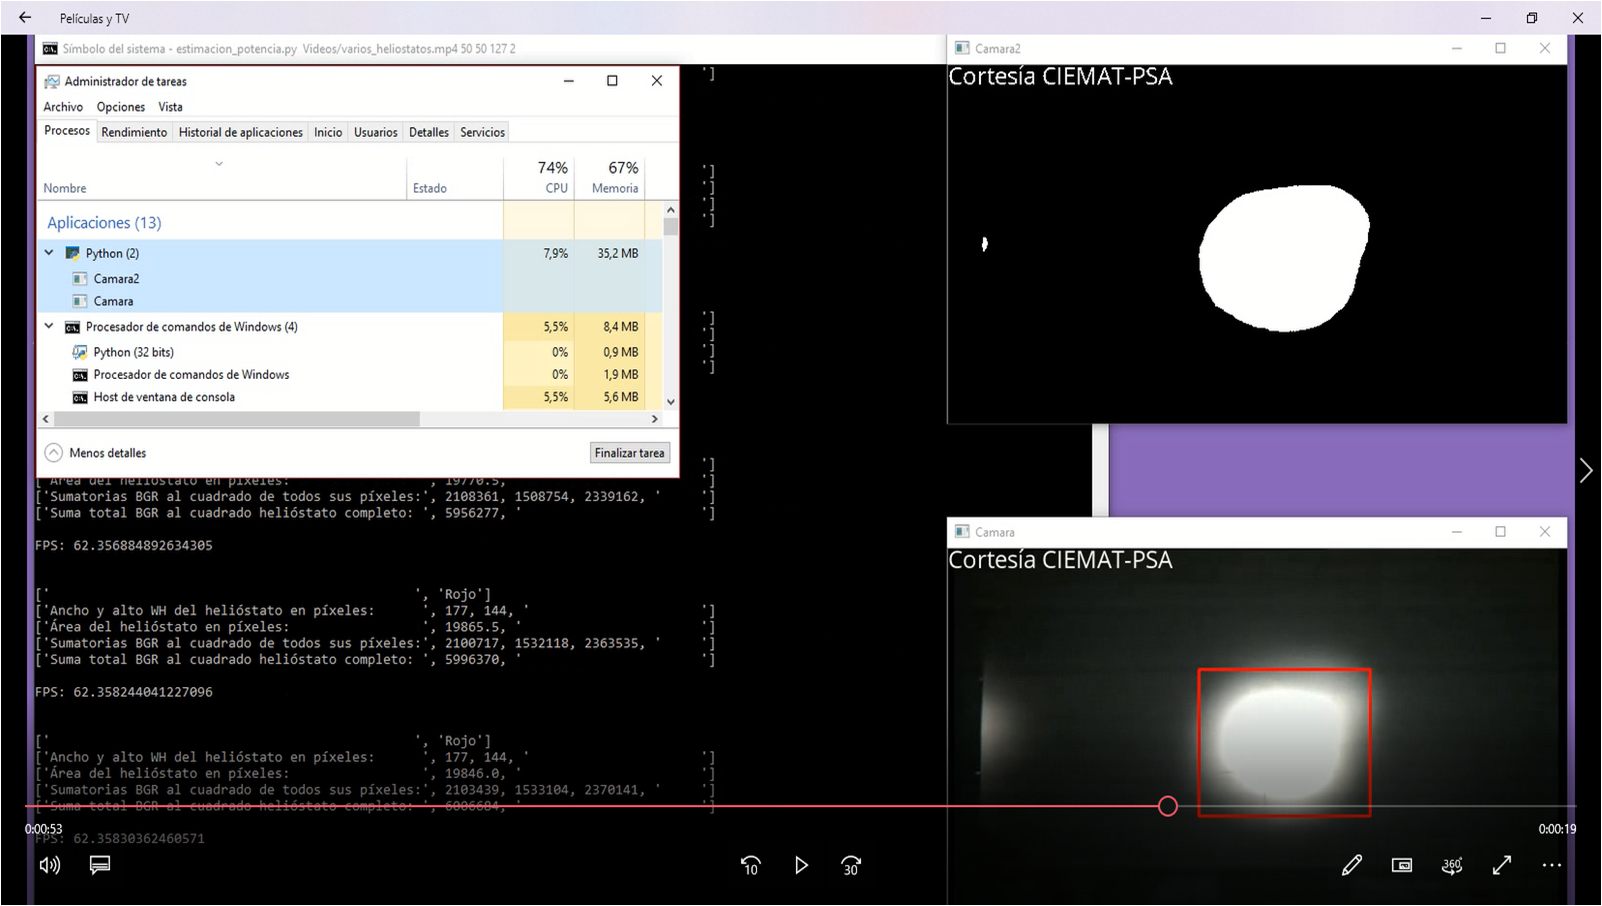
\includegraphics[width=\textwidth]{CapturasRendimientoSoftware1/Imagen15.png}
	\caption{Instante de tiempo 15 de la ejecución del software para el vídeo 'varios\_heliostatos.mp4'.
	\label{fig:CapturasRendimientoSoftware1/Imagen15.png}}
\end{figure}

Figura \ref{fig:CapturasRendimientoSoftware1/Imagen15.png}. Cuando el helióstato de la izquierda ya casi ni se ve porque este se ha separado bastante del helióstato del centro del vídeo, Python consume un 7,9\% de CPU y 35,2 MB de memoria RAM, mientras que la terminal de Windows consume un 5,5\% de CPU y 8,4 MB de memoria RAM. Los FPS son de 62,35.\\[20pt]

\begin{figure}[h!]
  	\centering
	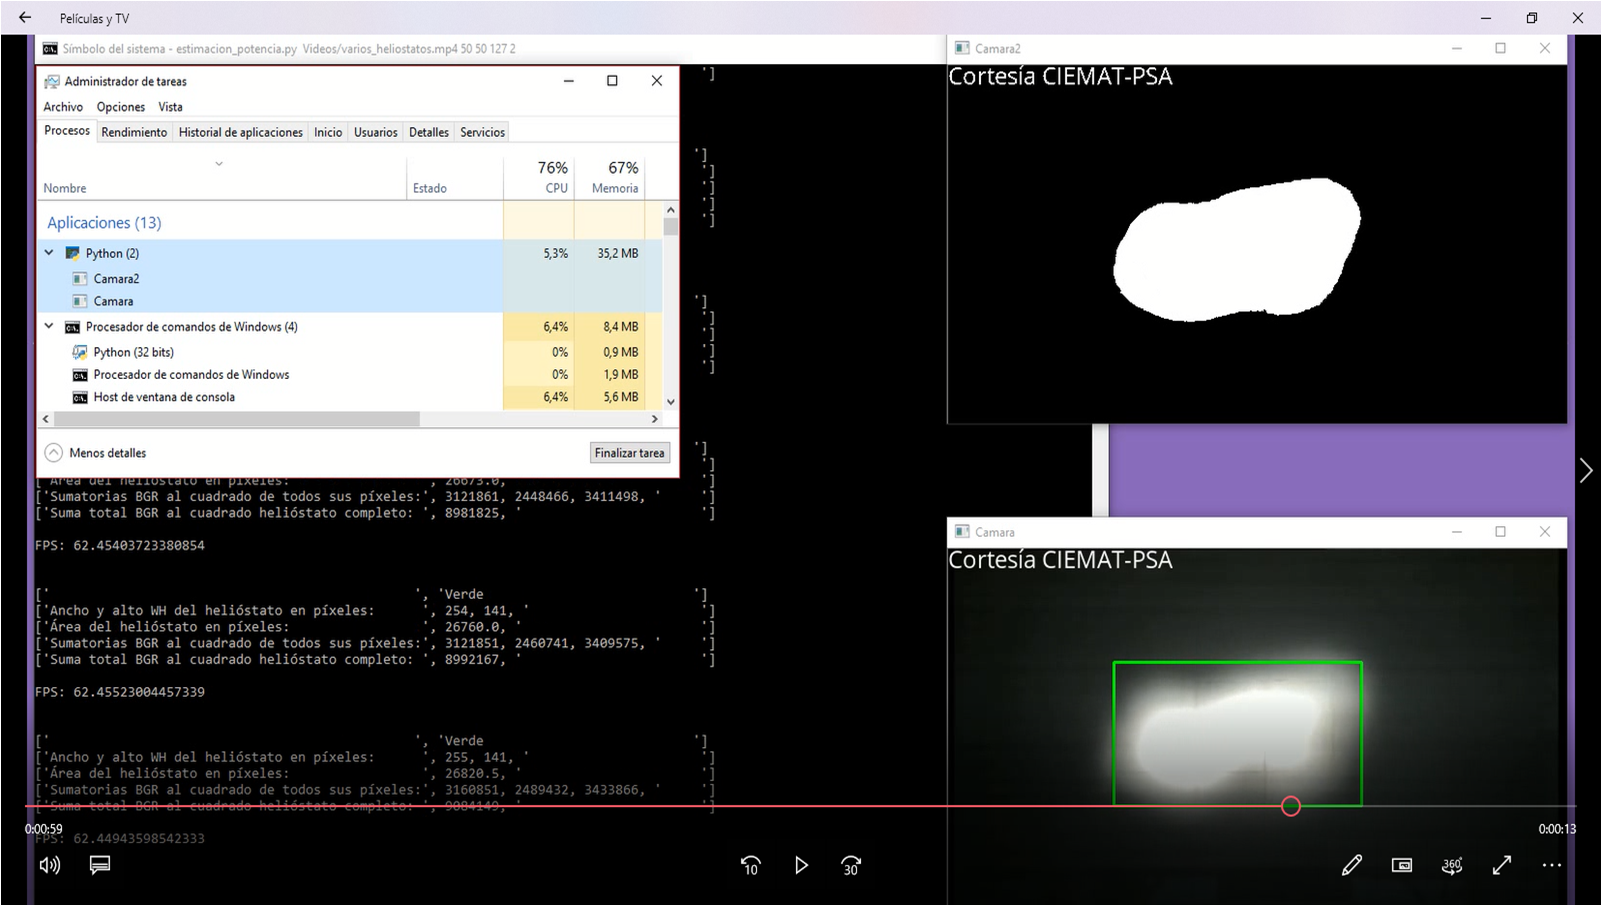
\includegraphics[width=\textwidth]{CapturasRendimientoSoftware1/Imagen16.png}
	\caption{Instante de tiempo 16 de la ejecución del software para el vídeo 'varios\_heliostatos.mp4'.
	\label{fig:CapturasRendimientoSoftware1/Imagen16.png}}
\end{figure}

Figura \ref{fig:CapturasRendimientoSoftware1/Imagen16.png}. Cuando otro (el tercero ya) de los helióstatos fusionados con el helióstato del centro del vídeo trata de salir del mismo (todavía no se ha completado este procedimiento). Python consume un 5,3\% de CPU y 35,2 MB de memoria RAM, mientras que la terminal de Windows consume un 6,4\% de CPU y 8,4 MB de memoria RAM. Los FPS son de 62,45.\\[20pt]

\begin{figure}[h!]
  	\centering
	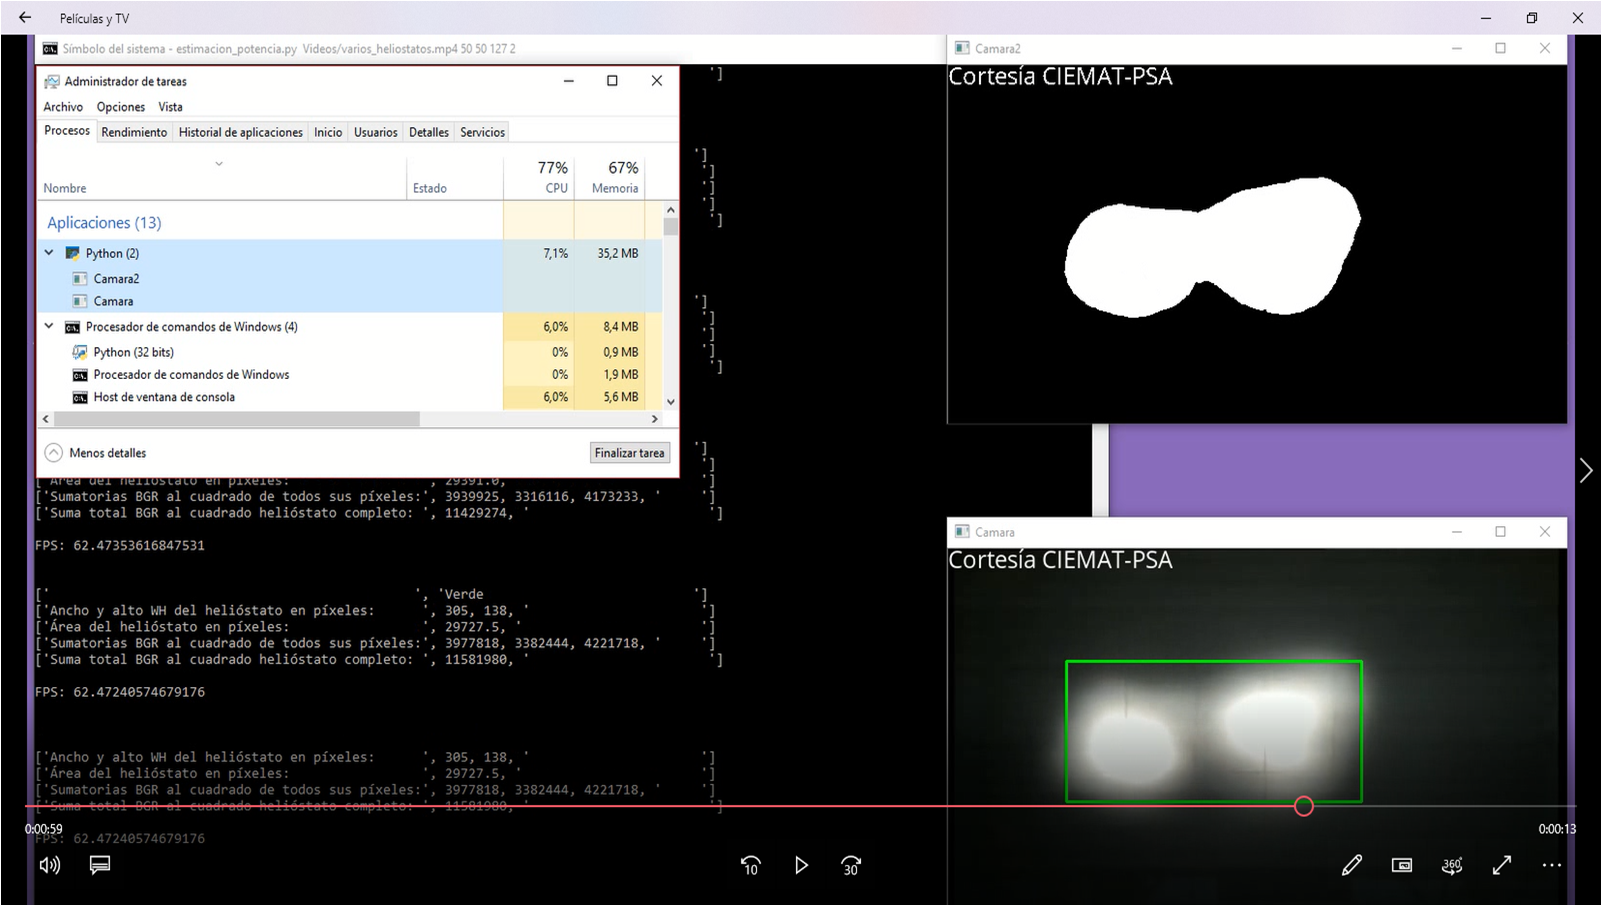
\includegraphics[width=\textwidth]{CapturasRendimientoSoftware1/Imagen17.png}
	\caption{Instante de tiempo 17 de la ejecución del software para el vídeo 'varios\_heliostatos.mp4'.
	\label{fig:CapturasRendimientoSoftware1/Imagen17.png}}
\end{figure}

Figura \ref{fig:CapturasRendimientoSoftware1/Imagen17.png}. Cuando los dos helióstatos están a punto de separarse entre sí. Python consume un 7,1\% de CPU y 35,2 MB de memoria RAM, mientras que la terminal de Windows consume un 6\% de CPU y 8,4 MB de memoria RAM. Los FPS son de 62,47.\\[20pt]

\begin{figure}[h!]
  	\centering
	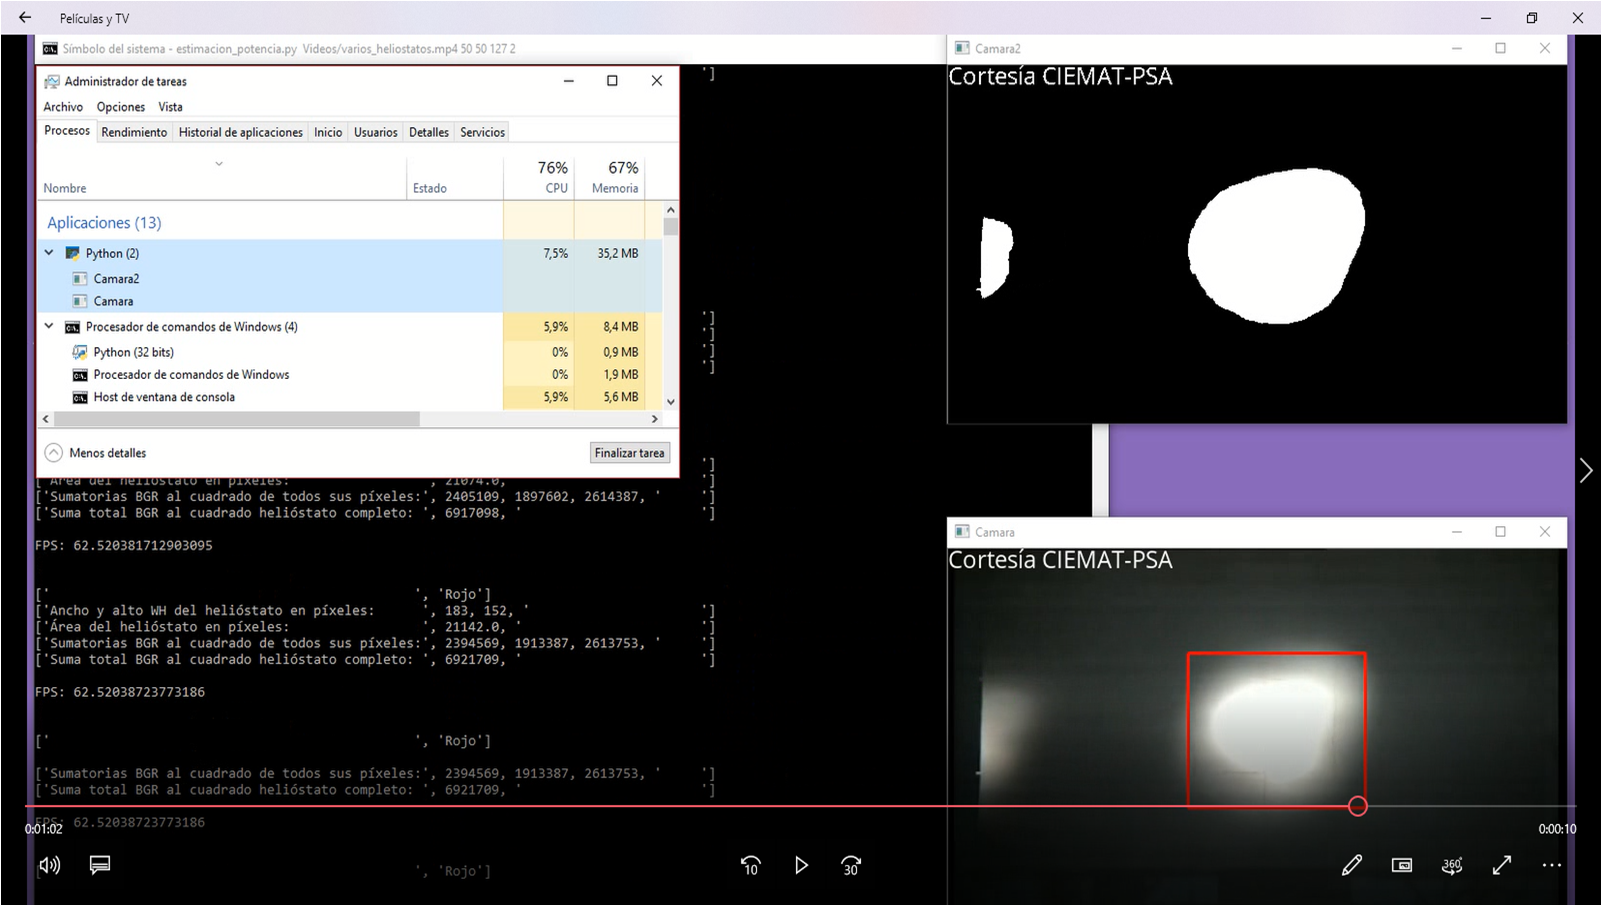
\includegraphics[width=\textwidth]{CapturasRendimientoSoftware1/Imagen18.png}
	\caption{Instante de tiempo 18 de la ejecución del software para el vídeo 'varios\_heliostatos.mp4'.
	\label{fig:CapturasRendimientoSoftware1/Imagen18.png}}
\end{figure}

Figura \ref{fig:CapturasRendimientoSoftware1/Imagen18.png}. Cuando el helióstato de la izquierda ya casi ni se ve porque este se ha separado bastante del helióstato del centro del vídeo, Python consume un 7,5\% de CPU y 35,2 MB de memoria RAM, mientras que la terminal de Windows consume un 5,9\% de CPU y 8,4 MB de memoria RAM. Los FPS son de 62,52.\\[20pt]

\begin{figure}[h!]
  	\centering
	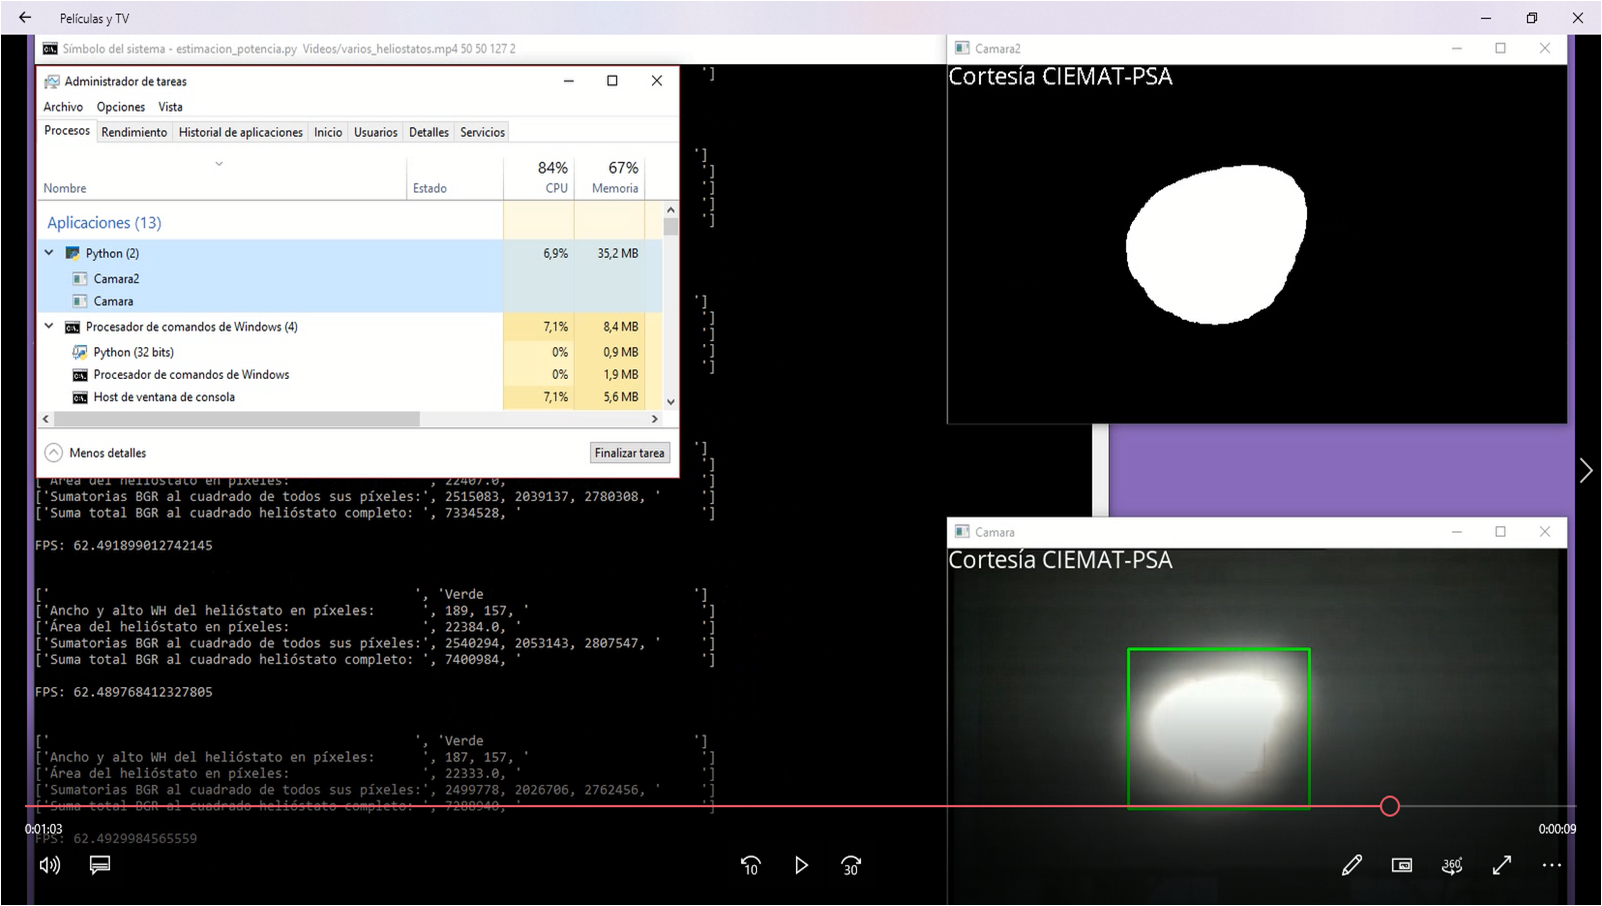
\includegraphics[width=\textwidth]{CapturasRendimientoSoftware1/Imagen19.png}
	\caption{Instante de tiempo 19 de la ejecución del software para el vídeo 'varios\_heliostatos.mp4'.
	\label{fig:CapturasRendimientoSoftware1/Imagen19.png}}
\end{figure}

Figura \ref{fig:CapturasRendimientoSoftware1/Imagen19.png}. Cuando el helióstato del centro del vídeo, el último de todos, empieza a trasladarse hacia la izquierda con el fin de salirse del vídeo, Python consume un 6,9\% de CPU y 35,2 MB de memoria RAM, mientras que la terminal de Windows consume un 7,1\% de CPU y 8,4 MB de memoria RAM. Los FPS son de 62,49.\\[20pt]

\begin{figure}[h!]
  	\centering
	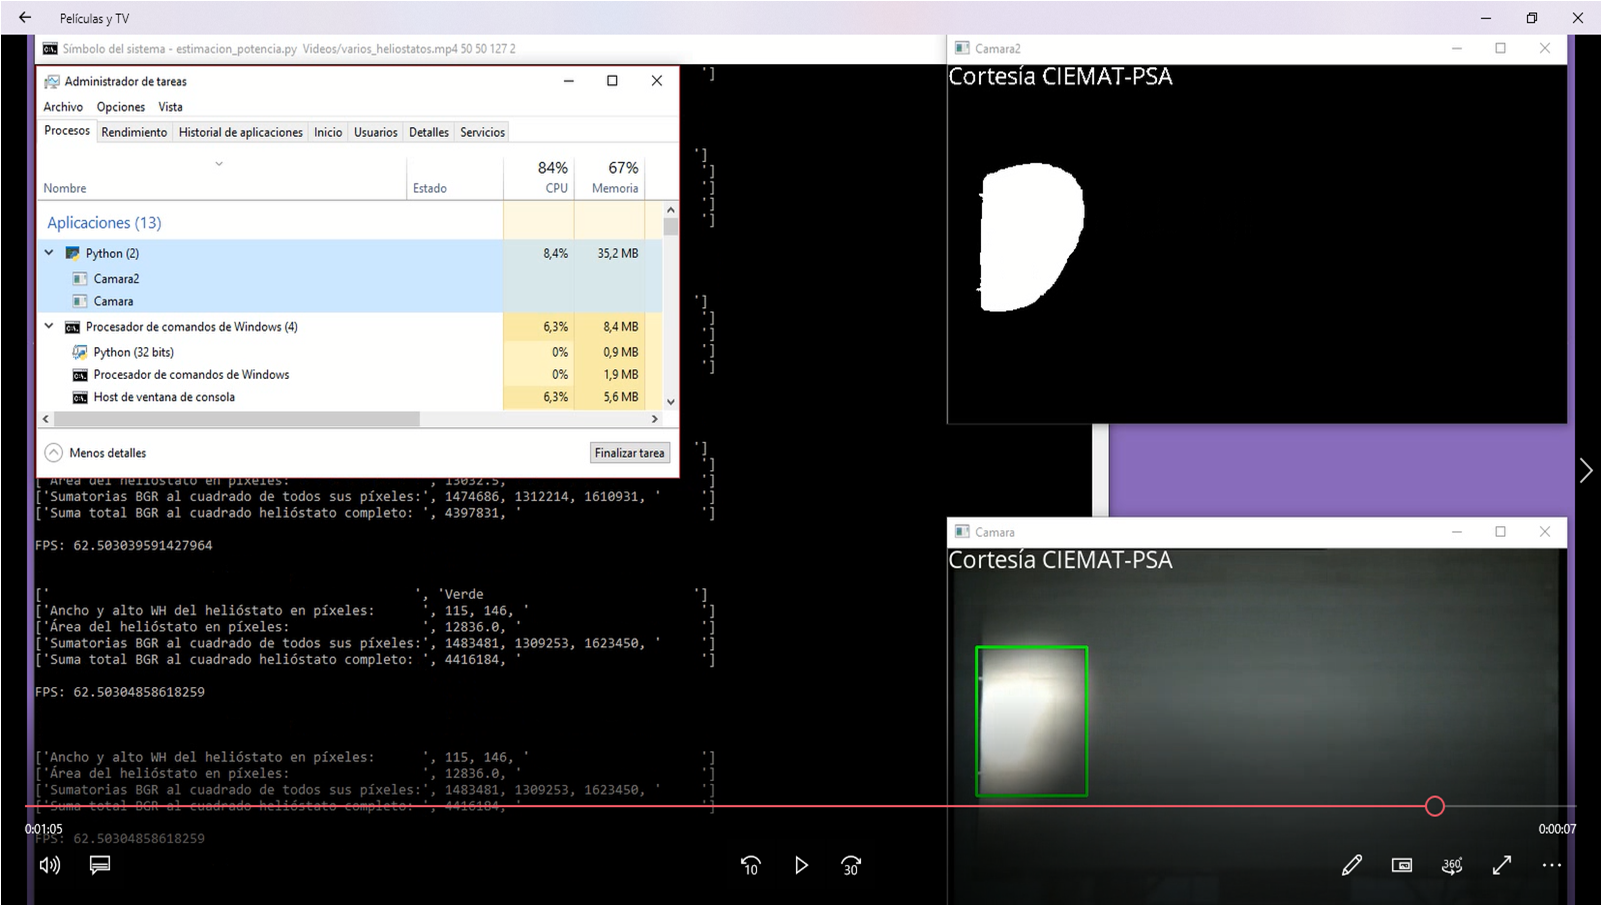
\includegraphics[width=\textwidth]{CapturasRendimientoSoftware1/Imagen20.png}
	\caption{Instante de tiempo 20 de la ejecución del software para el vídeo 'varios\_heliostatos.mp4'.
	\label{fig:CapturasRendimientoSoftware1/Imagen20.png}}
\end{figure}

Figura \ref{fig:CapturasRendimientoSoftware1/Imagen20.png}. Cuando dicho helióstato está a punto de desaparecer del vídeo (aún se muestra parcialmente a la izquierda del mismo), Python consume un 8,4\% de CPU y 35,2 MB de memoria RAM, mientras que la terminal de Windows consume un 6,3\% de CPU y 8,4 MB de memoria RAM. Los FPS son de 62,50.\\[20pt]

\begin{figure}[h!]
  	\centering
	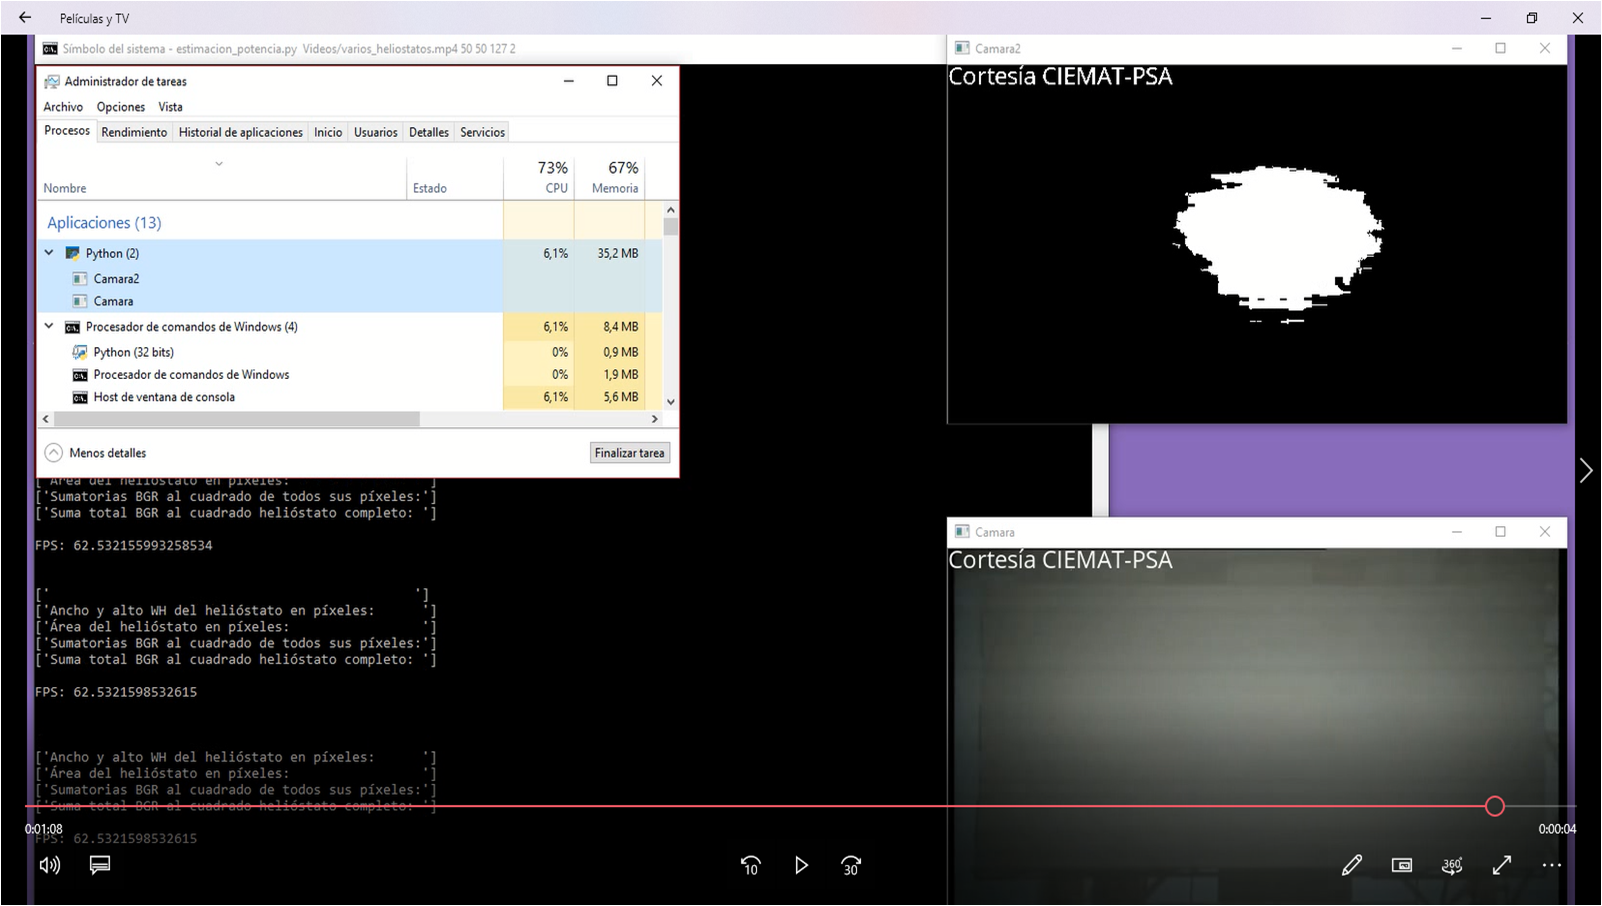
\includegraphics[width=\textwidth]{CapturasRendimientoSoftware1/Imagen21.png}
	\caption{Instante de tiempo 21 de la ejecución del software para el vídeo 'varios\_heliostatos.mp4'.
	\label{fig:CapturasRendimientoSoftware1/Imagen21.png}}
\end{figure}

Figura \ref{fig:CapturasRendimientoSoftware1/Imagen21.png}. Cuando finalmente no permanecen helióstatos en el vídeo (final del mismo, ya se han ido todos), Python consume un 6,1\% de CPU y 35,2 MB de memoria RAM, mientras que la terminal de Windows consume un 6,1\% de CPU y 8,4 MB de memoria RAM. Los FPS son de 62,53.\\[20pt]

\subsection{Cargando el vídeo 'heliostato.MOV'}

Se inicia la ejecución del software desde la terminal de Windows, estando en el directorio que contiene dicho software a ejecutar, y usando esta vez el comando \verb|estimacion_potencia.py Videos/heliostato.MOV 50 50 200 1|.

\begin{figure}[h!]
  	\centering
	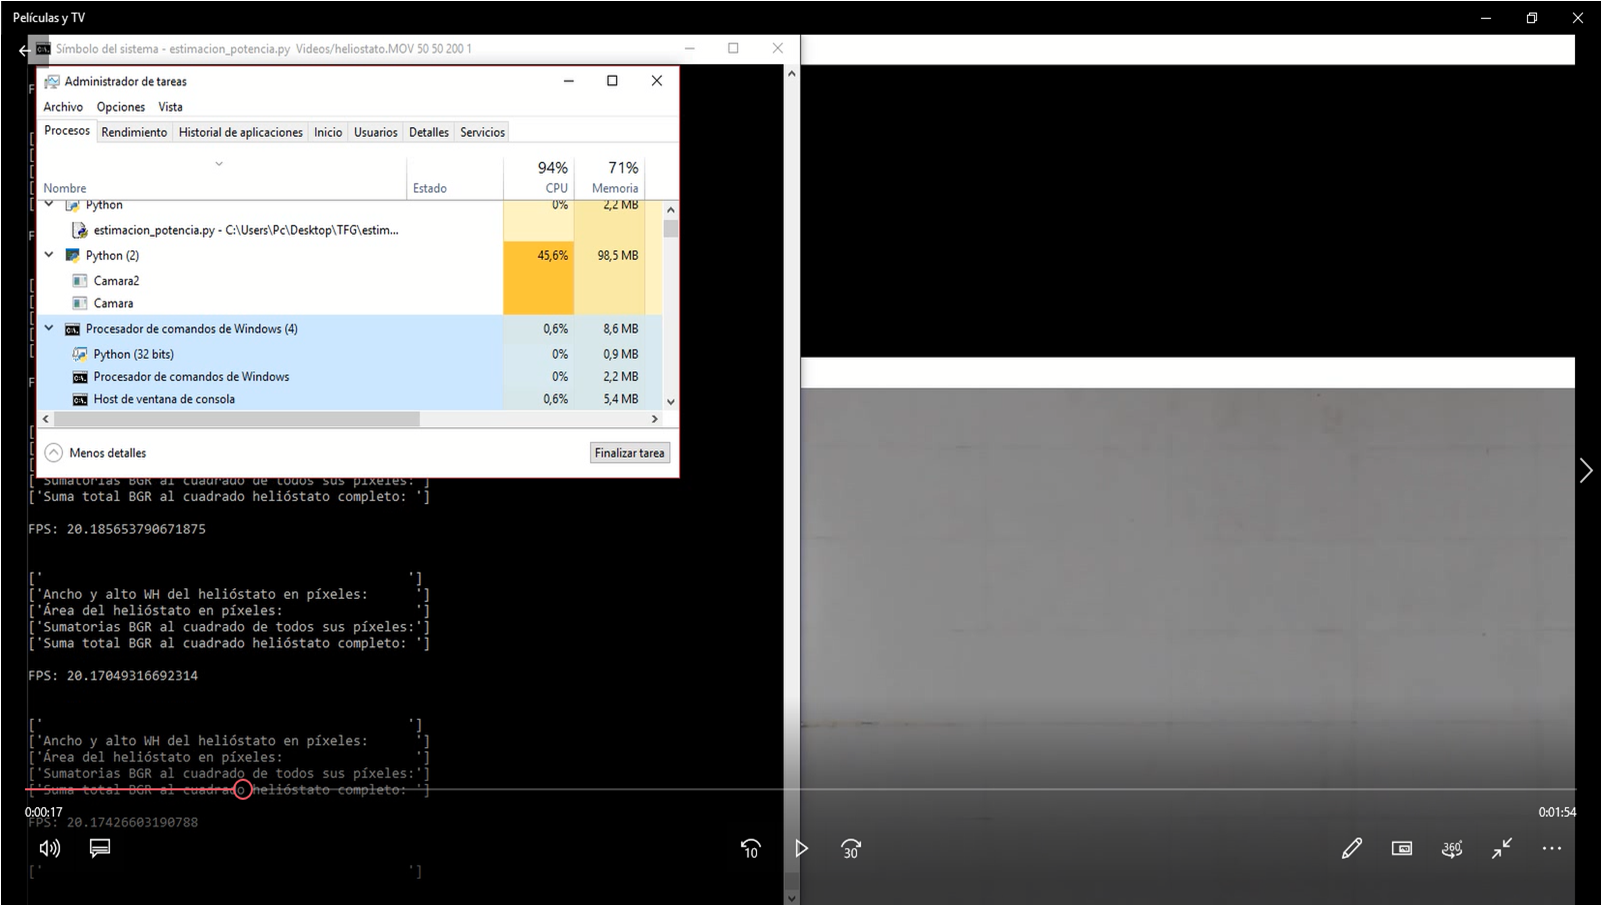
\includegraphics[width=\textwidth]{CapturasRendimientoSoftware2/Imagen1.png}
	\caption{Instante de tiempo 1 de la ejecución del software para el vídeo 'heliostato.MOV'.
	\label{fig:CapturasRendimientoSoftware2/Imagen1.png}}
\end{figure}

Figura \ref{fig:CapturasRendimientoSoftware2/Imagen1.png}. Nada más iniciar la ejecución del software, cuando todavía no han pasado por el vídeo los helióstatos, ni siquiera el primero, Python consume un 45,6\% de CPU y 98,5 MB de memoria RAM, mientras que la terminal de Windows consume un 0,6\% de CPU y 8,6 MB de memoria RAM. Los FPS son de 20,18.\\[20pt]

\begin{figure}[h!]
  	\centering
	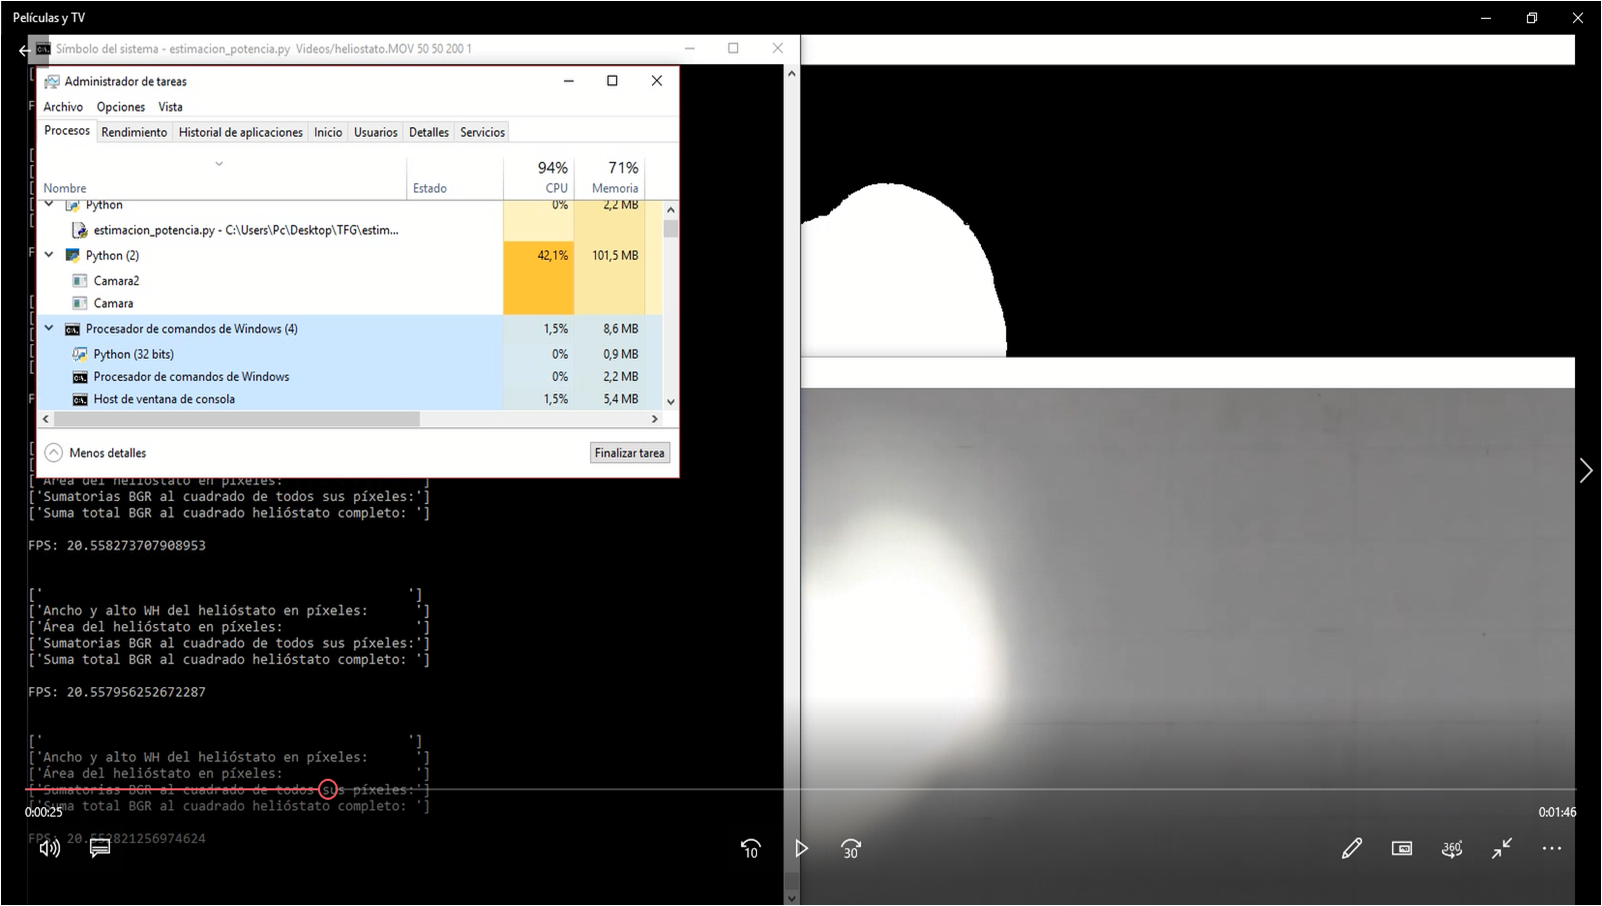
\includegraphics[width=\textwidth]{CapturasRendimientoSoftware2/Imagen2.png}
	\caption{Instante de tiempo 2 de la ejecución del software para el vídeo 'heliostato.MOV'.
	\label{fig:CapturasRendimientoSoftware2/Imagen2.png}}
\end{figure}

Figura \ref{fig:CapturasRendimientoSoftware2/Imagen2.png}. Cuando está entrando el primer helióstato en el vídeo (todavía no ha entrado completamente, sino parcialmente), Python consume un 42,1\% de CPU y 101,5 MB de memoria RAM, mientras que la terminal de Windows consume un 1,5\% de CPU y 8,6 MB de memoria RAM. Los FPS son de 20,55.\\[20pt]

\begin{figure}[h!]
  	\centering
	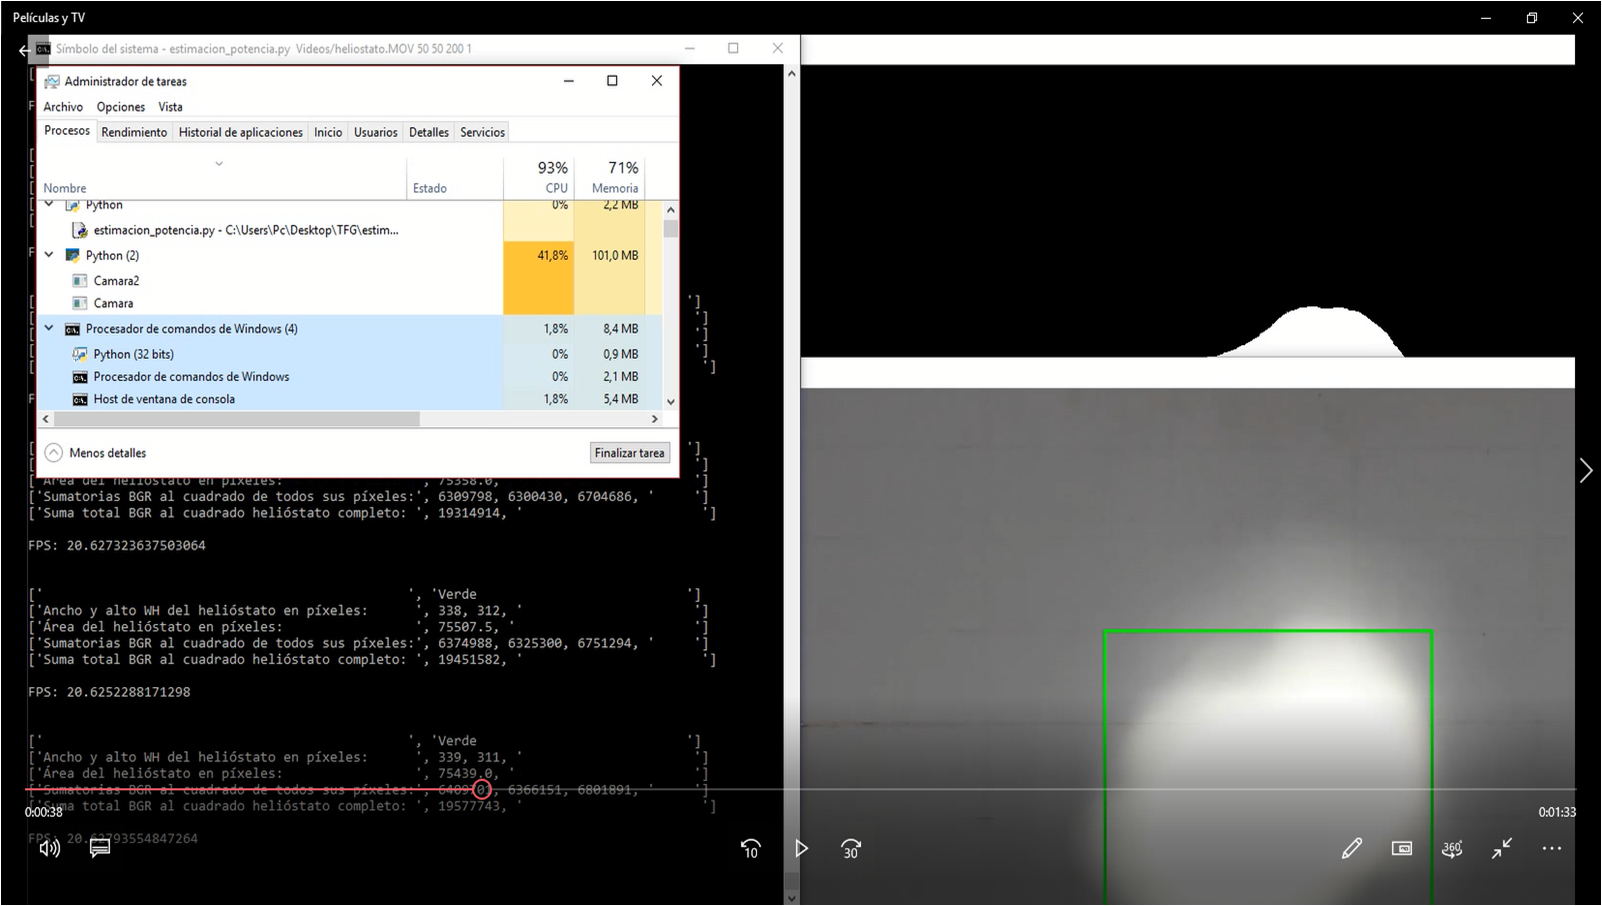
\includegraphics[width=\textwidth]{CapturasRendimientoSoftware2/Imagen3.png}
	\caption{Instante de tiempo 3 de la ejecución del software para el vídeo 'heliostato.MOV'.
	\label{fig:CapturasRendimientoSoftware2/Imagen3.png}}
\end{figure}

Figura \ref{fig:CapturasRendimientoSoftware2/Imagen3.png}. Cuando el primer helióstato ya ha llegado al centro del vídeo, Python consume un 41,8\% de CPU y 101,0 MB de memoria RAM, mientras que la terminal de Windows consume un 1,8\% de CPU y 8,4 MB de memoria RAM. Los FPS son de 20,62.\\[20pt]

\begin{figure}[h!]
  	\centering
	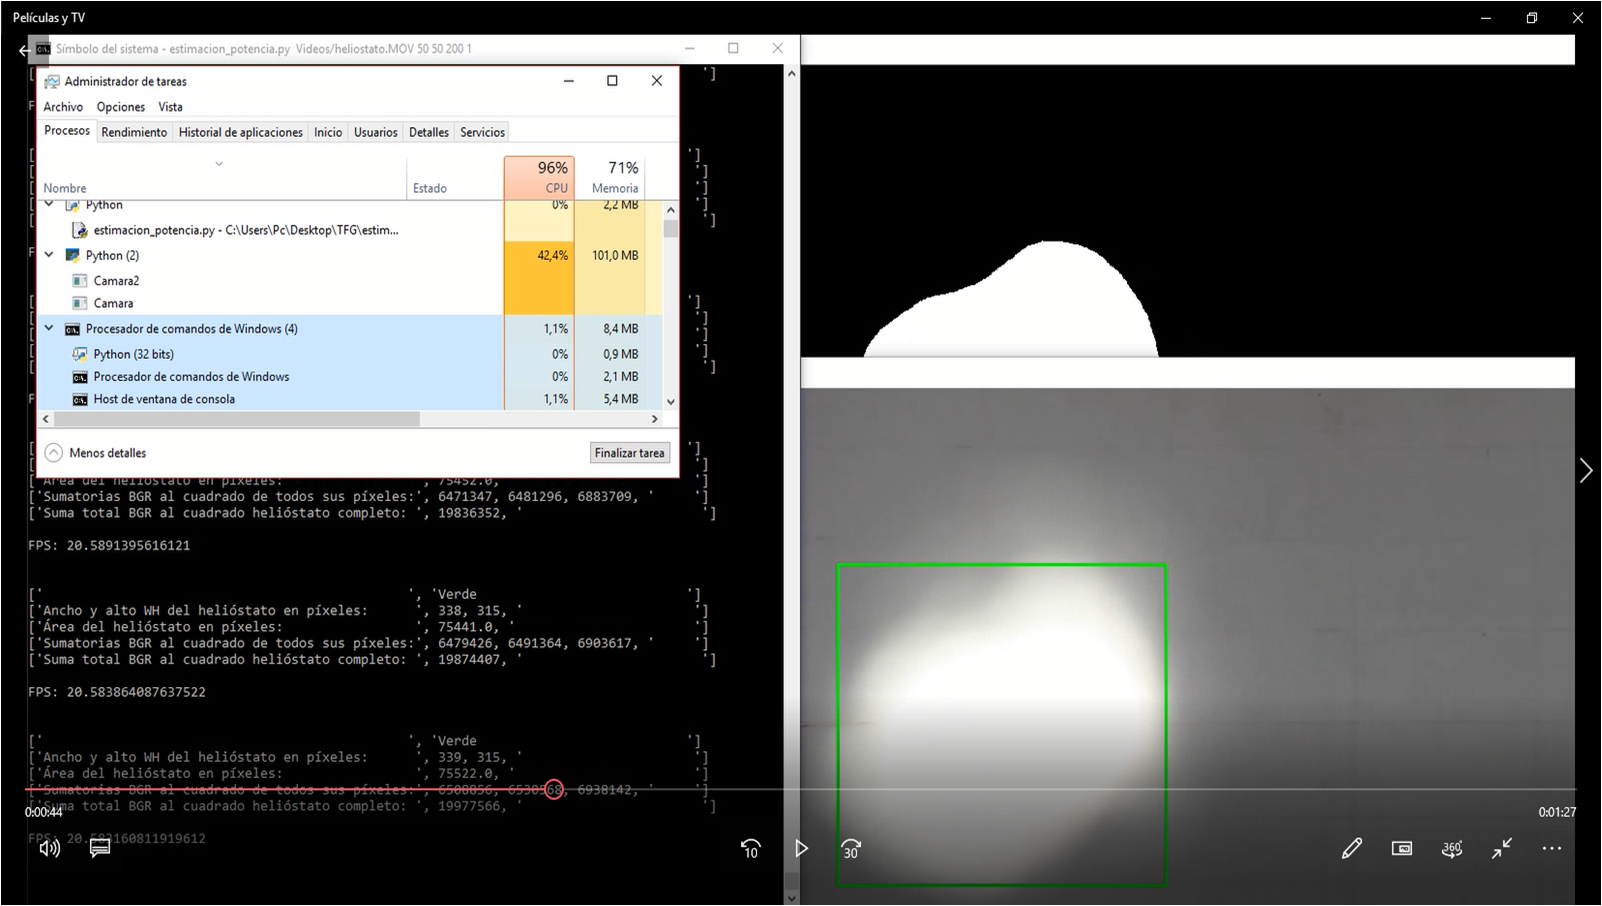
\includegraphics[width=\textwidth]{CapturasRendimientoSoftware2/Imagen4.png}
	\caption{Instante de tiempo 4 de la ejecución del software para el vídeo 'heliostato.MOV'.
	\label{fig:CapturasRendimientoSoftware2/Imagen4.png}}
\end{figure}

Figura \ref{fig:CapturasRendimientoSoftware2/Imagen4.png}. Cuando el primer helióstato tiende a irse del centro del vídeo, Python consume un 42,4\% de CPU y 101 MB de memoria RAM, mientras que la terminal de Windows consume un 1,1\% de CPU y 8,4 MB de memoria RAM. Los FPS son de 20,58.\\[20pt]

\begin{figure}[h!]
  	\centering
	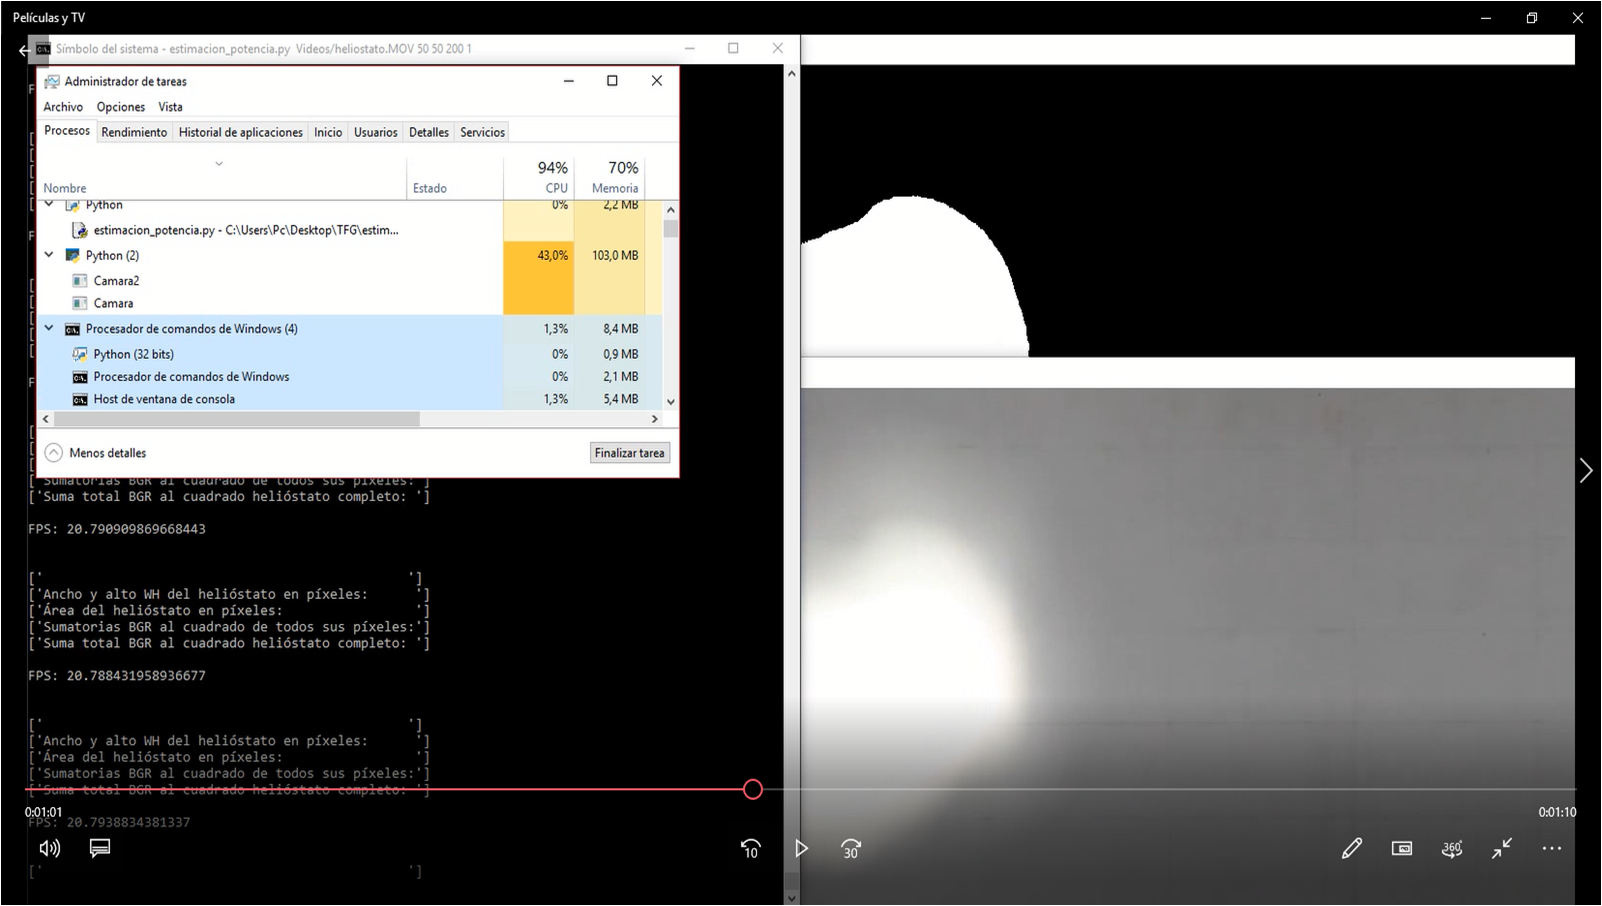
\includegraphics[width=\textwidth]{CapturasRendimientoSoftware2/Imagen5.png}
	\caption{Instante de tiempo 5 de la ejecución del software para el vídeo 'heliostato.MOV'.
	\label{fig:CapturasRendimientoSoftware2/Imagen5.png}}
\end{figure}

Figura \ref{fig:CapturasRendimientoSoftware2/Imagen5.png}. Cuando está llegando al centro del vídeo un segundo helióstato desde la izquierda, Python consume un 43\% de CPU y 103 MB de memoria RAM, mientras que la terminal de Windows consume un 1,3\% de CPU y 8,4 MB de memoria RAM. Los FPS son de 20,79.\\[20pt]

\begin{figure}[h!]
  	\centering
	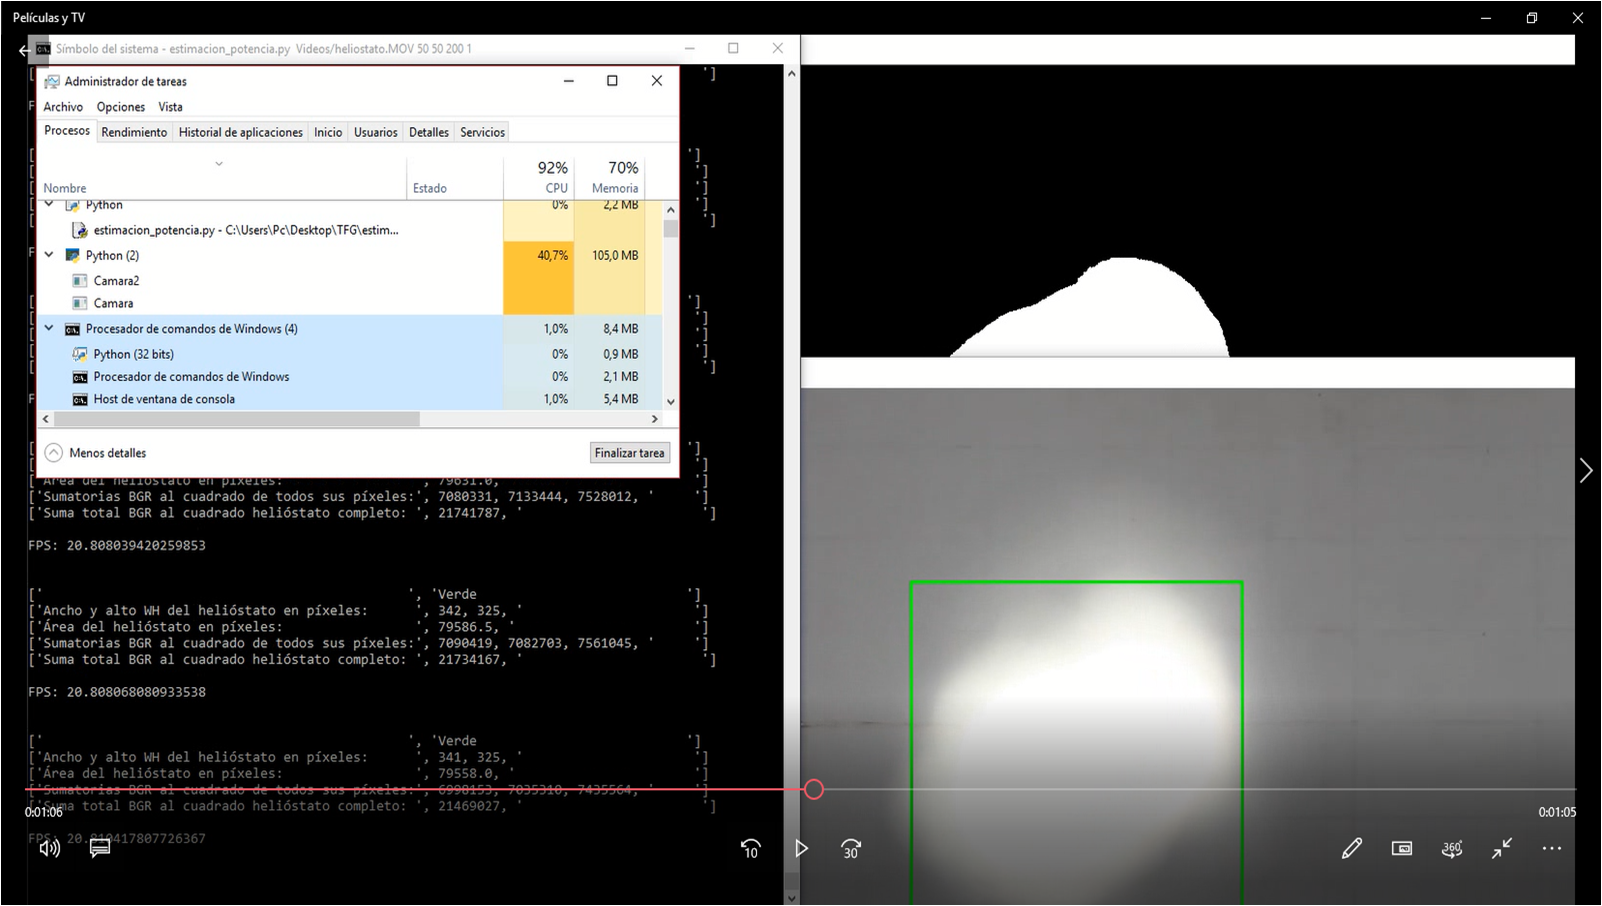
\includegraphics[width=\textwidth]{CapturasRendimientoSoftware2/Imagen6.png}
	\caption{Instante de tiempo 6 de la ejecución del software para el vídeo 'heliostato.MOV'.
	\label{fig:CapturasRendimientoSoftware2/Imagen6.png}}
\end{figure}

Figura \ref{fig:CapturasRendimientoSoftware2/Imagen6.png}. Cuando el segundo helióstato se ha aproximado un poco más al centro del vídeo (respecto al instante de tiempo anterior), Python consume un 40,7\% de CPU y 105 MB de memoria RAM, mientras que la terminal de Windows consume un 1\% de CPU y 8,4 MB de memoria RAM. Los FPS son de 20,8.\\[20pt]

\begin{figure}[h!]
  	\centering
	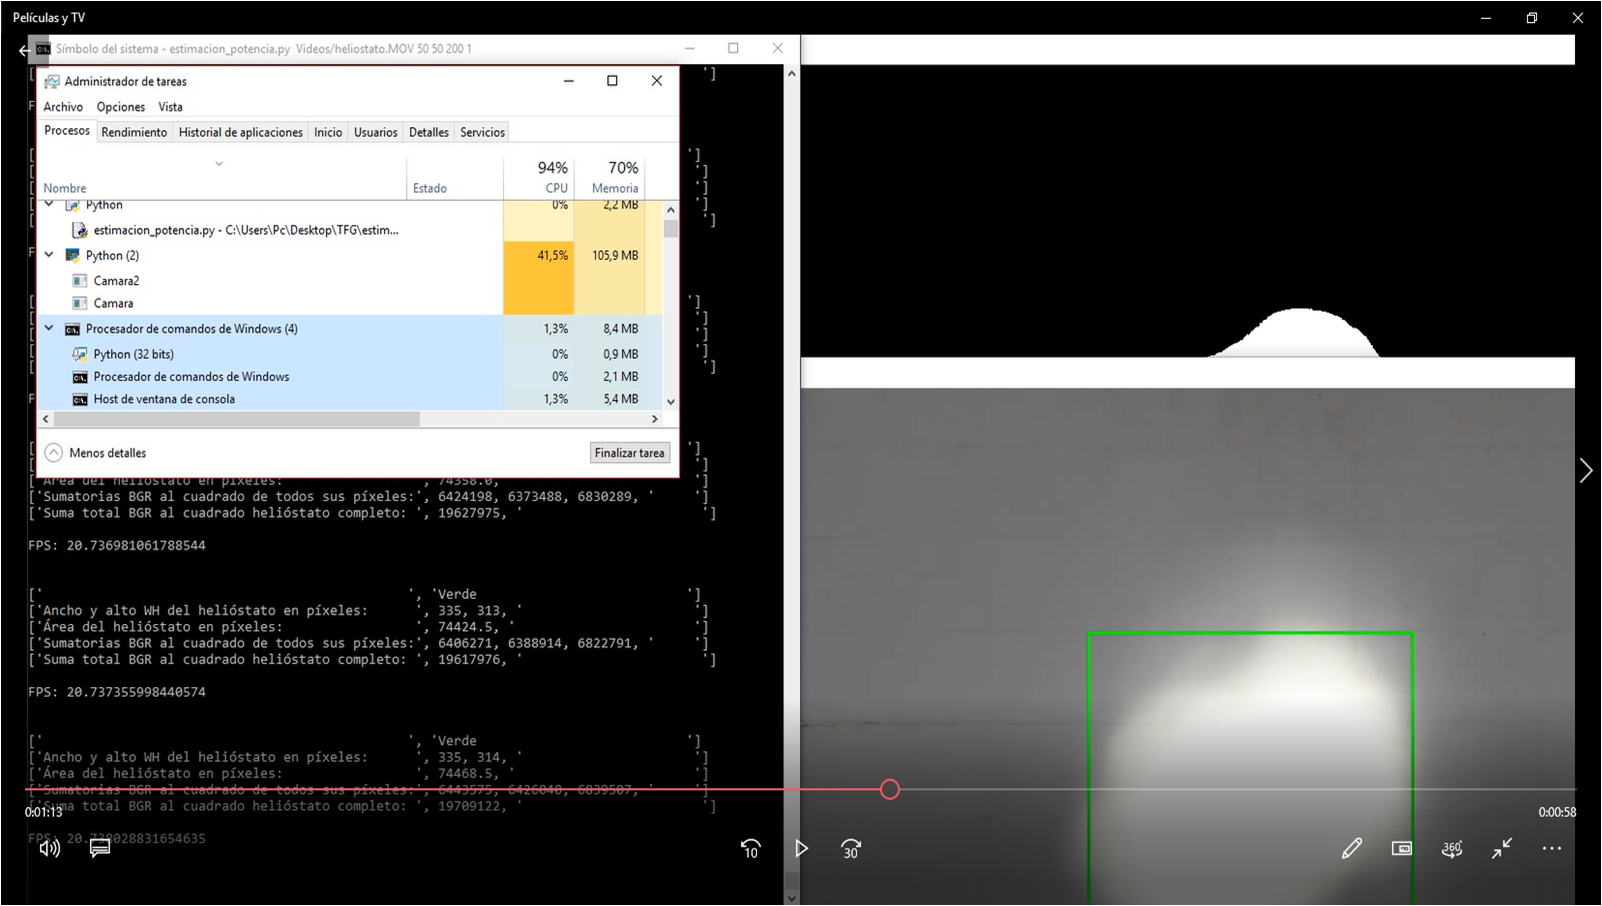
\includegraphics[width=\textwidth]{CapturasRendimientoSoftware2/Imagen7.png}
	\caption{Instante de tiempo 7 de la ejecución del software para el vídeo 'heliostato.MOV'.
	\label{fig:CapturasRendimientoSoftware2/Imagen7.png}}
\end{figure}

Figura \ref{fig:CapturasRendimientoSoftware2/Imagen7.png}. Cuando el segundo helióstato ya ha llegado al centro del vídeo, Python consume un 41,5\% de CPU y 105,9 MB de memoria RAM, mientras que la terminal de Windows consume un 1,3\% de CPU y 8,4 MB de memoria RAM. Los FPS son de 20,73.\\[20pt]

\begin{figure}[h!]
  	\centering
	\includegraphics[width=\textwidth]{CapturasRendimientoSoftware2/Imagen8.png}
	\caption{Instante de tiempo 8 de la ejecución del software para el vídeo 'heliostato.MOV'.
	\label{fig:CapturasRendimientoSoftware2/Imagen8.png}}
\end{figure}

Figura \ref{fig:CapturasRendimientoSoftware2/Imagen8.png}. Cuando el segundo helióstato tiende a irse del centro del vídeo, Python consume un 36,2\% de CPU y 103,1 MB de memoria RAM, mientras que la terminal de Windows consume un 0,9\% de CPU y 8,4 MB de memoria RAM. Los FPS son de 20,58.\\[20pt]

\begin{figure}[h!]
  	\centering
	\includegraphics[width=\textwidth]{CapturasRendimientoSoftware2/Imagen9.png}
	\caption{Instante de tiempo 9 de la ejecución del software para el vídeo 'heliostato.MOV'.
	\label{fig:CapturasRendimientoSoftware2/Imagen9.png}}
\end{figure}

Figura \ref{fig:CapturasRendimientoSoftware2/Imagen9.png}. Cuando el segundo helióstato ya ha abandonado el vídeo y aún no ha llegado el tercero, Python consume un 40,3\% de CPU y 102,0 MB de memoria RAM, mientras que la terminal de Windows consume un 0,8\% de CPU y 8,4 MB de memoria RAM. Los FPS son de 20,59.\\[20pt]

\begin{figure}[h!]
  	\centering
	\includegraphics[width=\textwidth]{CapturasRendimientoSoftware2/Imagen10.png}
	\caption{Instante de tiempo 10 de la ejecución del software para el vídeo 'heliostato.MOV'.
	\label{fig:CapturasRendimientoSoftware2/Imagen10.png}}
\end{figure}

Figura \ref{fig:CapturasRendimientoSoftware2/Imagen10.png}. Cuando el tercer helióstato está entrando en el vídeo (todavía no ha entrado completamente, sino parcialmente), Python consume un 44,3\% de CPU y 105,3 MB de memoria RAM, mientras que la terminal de Windows consume un 0\% de CPU y 8,4 MB de memoria RAM. Los FPS son de 20,65.\\[20pt]

\begin{figure}[h!]
  	\centering
	\includegraphics[width=\textwidth]{CapturasRendimientoSoftware2/Imagen11.png}
	\caption{Instante de tiempo 11 de la ejecución del software para el vídeo 'heliostato.MOV'.
	\label{fig:CapturasRendimientoSoftware2/Imagen11.png}}
\end{figure}

Figura \ref{fig:CapturasRendimientoSoftware2/Imagen11.png}. Cuando el tercer helióstato está a punto de alcanzar el centro del vídeo, Python consume un 42,9\% de CPU y 101,1 MB de memoria RAM, mientras que la terminal de Windows consume un 1,3\% de CPU y 8,4 MB de memoria RAM. Los FPS son de 20,67.\\[20pt]

\begin{figure}[h!]
  	\centering
	\includegraphics[width=\textwidth]{CapturasRendimientoSoftware2/Imagen12.png}
	\caption{Instante de tiempo 12 de la ejecución del software para el vídeo 'heliostato.MOV'.
	\label{fig:CapturasRendimientoSoftware2/Imagen12.png}}
\end{figure}

Figura \ref{fig:CapturasRendimientoSoftware2/Imagen12.png}. Cuando el tercer helióstato se está alejando del centro del vídeo, Python consume un 39,2\% de CPU y 103,1 MB de memoria RAM, mientras que la terminal de Windows consume un 1,5\% de CPU y 8,4 MB de memoria RAM. Los FPS son de 20,64.\\[20pt]

\begin{figure}[h!]
  	\centering
	\includegraphics[width=\textwidth]{CapturasRendimientoSoftware2/Imagen13.png}
	\caption{Instante de tiempo 13 de la ejecución del software para el vídeo 'heliostato.MOV'.
	\label{fig:CapturasRendimientoSoftware2/Imagen13.png}}
\end{figure}

Figura \ref{fig:CapturasRendimientoSoftware2/Imagen13.png}. Cuando el tercer helióstato está a punto de abandonar el vídeo, Python consume un 42,8\% de CPU y 102,5 MB de memoria RAM, mientras que la terminal de Windows consume un 0,8\% de CPU y 8,4 MB de memoria RAM. Los FPS son de 20,65.\\[20pt]

\begin{figure}[h!]
  	\centering
	\includegraphics[width=\textwidth]{CapturasRendimientoSoftware2/Imagen14.png}
	\caption{Instante de tiempo 14 de la ejecución del software para el vídeo 'heliostato.MOV'.
	\label{fig:CapturasRendimientoSoftware2/Imagen14.png}}
\end{figure}

Figura \ref{fig:CapturasRendimientoSoftware2/Imagen14.png}. Cuando no hay ningún helióstato en el vídeo (todos ya han pasado por él, y no quedan más), Python consume un 46,2\% de CPU y 104,3 MB de memoria RAM, mientras que la terminal de Windows consume un 0,3\% de CPU y 8,4 MB de memoria RAM. Los FPS son de 20,68.\\[20pt]

\begin{figure}[h!]
  	\centering
	\includegraphics[width=\textwidth]{CapturasRendimientoSoftware1/GraficasRendimientoSoftware1.PNG}
	\caption{Histograma para el caso/comando 'estimacion\_potencia.py Videos/varios\_heliostatos.mp4 50 50 127 2'.
	\label{fig:CapturasRendimientoSoftware1/GraficasRendimientoSoftware1.PNG}}
\end{figure}

\begin{figure}[h!]
  	\centering
	\includegraphics[width=\textwidth]{CapturasRendimientoSoftware2/GraficasRendimientoSoftware2.PNG}
	\caption{Histograma para el caso/comando 'estimacion\_potencia.py Videos/heliostato.MOV 50 50 200 1'.
	\label{fig:CapturasRendimientoSoftware2/GraficasRendimientoSoftware2.PNG}}
\end{figure}

Las figuras \ref{fig:CapturasRendimientoSoftware1/GraficasRendimientoSoftware1.PNG} y \ref{fig:CapturasRendimientoSoftware2/GraficasRendimientoSoftware2.PNG} muestran dos histogramas a modo resumen de los resultados comentados en este apartado.

\section{Plataformas que son capaces de ejecutar el software}

El software está escrito en lenguaje de programación Python, y una de las características de Python es que es un lenguaje multiplataforma. Esto significa que, aunque originalmente Python se diseñó para Unix, cualquier sistema es compatible con el lenguaje siempre y cuando exista un intérprete programado para él. Además, hay diversas versiones de Python en muchos sistemas informáticos distintos.

\section{Ejemplos de ejecuciones y comentarios sobre sus resultados}

\subsection{Cargando el vídeo 'variosHeliostatos.mp4'}

Al iniciar la ejecución del software desde la terminal de Windows, estando en el directorio que contiene dicho software a ejecutar, y usando el comando \verb|estimacion_potencia.py Videos/varios_heliostatos.mp4 50 50 127 2|, ocurre lo siguiente:

Cuando un helióstato comienza a entrar en el vídeo de helióstatos, el programa todavía no lo reencuadra en dicho vídeo ni lo analiza. Esto se debe a que, en este instante de tiempo, el helióstato mostrado en el vídeo aún no es de ancho y alto 50 píxeles o más, tal y como solicitó el usuario por parámetros en la consola. De forma análoga ocurre cuando un helióstato está a punto de salir del vídeo: en ese instante apenas se muestra el helióstato en el vídeo, y el ancho o el alto mostrados no son mayores de 50 píxeles, siendo ignorado por el programa. También debe cumplirse el valor de umbral proporcionado por parámetro para el análisis del helióstato, 127. De lo contrario, si el helióstato se muestra en su totalidad en el vídeo, o por lo menos su ancho y alto en un instante determinado son mayores de 50 píxeles (y por supuesto el umbral del vídeo es al menos de 127), el programa lo reencuadra en el vídeo y lo analiza.

Por parámetro en la consola, se ha indicado también que se desea leer hasta un máximo de dos helióstatos por fotograma del vídeo, porque en este vídeo pueden mostrarse hasta dos helióstatos en un mismo fotograma. Si en vez de '2' se introduce '1', cuando aparezcan dos helióstatos en un mismo fotograma, simplemente se reencuadrará en el vídeo y procesará el helióstato situado a la izquierda, y no el de la derecha.

En el análisis de un helióstato, el programa calculará su ancho y alto, su área total (todo estos valores se miden en píxeles), la sumatoria acumulativa de los valores de cada componente BGR al cuadrado (cada componente por separado) de todo el helióstato, y esto mismo pero sumando las tres componentes resultantes entre sí. Los resultados de estos datos son mostrados por consola, para cada helióstato analizado. En la consola, dichos datos son representados textualmente así (respectivamente):

\begin{lstlisting}
Ancho y alto WH del helióstato en píxeles.
Área del helióstato en píxeles.
Sumatorias BGR al cuadrado de todos sus píxeles.
Suma total BGR al cuadrado helióstato completo.
\end{lstlisting}

En el análisis de un helióstato, además, el programa reencuadrará en el vídeo y en tiempo de ejecución los helióstatos que se están analizando actualmente. Si en el fotograma actual de dicho vídeo simplemente aparece un helióstato, se reencuadrará en color verde. De lo contrario, si aparecen dos helióstatos al mismo tiempo en un mismo fotograma, el helióstato de la izquierda se reencuadrará en verde y el de la derecha en rojo. En cualquiera de los casos, y tal y como se comentó antes, el programa analizará el o los helióstatos y mostrará sus resultados en la consola. Tener en cuenta que cuando se analizan dos helióstatos en un mismo fotograma, el programa mostrará sus respectivos resultados en la consola en dos columnas. La primera para el helióstato reencuadrado en verde, y la segunda para el helióstato reencuadrado en rojo. Finalmente, indicar que cuando dos helióstatos, en un mismo fotograma, están fusionados (parcialmente o totalmente) o rozándose, serán tratados y analizados como si fueran uno solo.

La tasa de fotogramas por segundo (FPS) es alta, de aproximadamente 60 FPS, porque se está procesando un vídeo de dimensiones reducidas, y gracias también al uso de matrices vectorizadas (biblioteca 'NumPy' de Python) para la carga, procesamiento y guardado de todos los datos de todos los píxeles de cada helióstato.

Todo este procedimiento se repite para todos los demás fotogramas del vídeo de helióstatos, hasta que se hayan leído todos sus fotogramas, finalizando así la ejecución del programa.

El contenido de este vídeo son de cuatro helióstatos que entran poco a poco en el vídeo desde el lado izquierdo, y se van ubicando en el centro. Los demás (y siguientes) helióstatos que también llegan desde la izquierda se solapan con el helióstato o helióstatos permanecidos en el centro de dicho vídeo. Cuando los cuatro helióstatos permanezcan solapados en el centro del vídeo, se irán separando, uno por uno, los helióstatos hacia la izquierda, saliéndose cada uno del vídeo, hasta que no queden ninguno.

\subsection{Cargando el vídeo 'heliostato.MOV'}

Al iniciar la ejecución del software desde la terminal de Windows, estando en el directorio que contiene dicho software a ejecutar, y usando esta vez el comando \verb|estimacion_potencia.py Videos/heliostato.MOV 50 50 200 1|, ocurre lo siguiente:

Para que el helióstato sea en esta ocasión reencuadrado en el vídeo y analizado, el nuevo umbral escogido es de 200, porque el nuevo vídeo tiene una tonalidad de color más clara. En el anterior caso, bastaba con un umbral de 127 porque aquel vídeo era más oscuro. El ancho y alto escogidos del helióstato, al igual que en el caso anterior, es de 50 por 50 píxeles.

Como en este vídeo aparece como máximo un único helióstato por fotograma, se indica por parámetro en la consola que se desea analizar esta vez 1 helióstato por fotograma (en vez de 2, como sucedía en el anterior caso). Si se escribe un número mayor a 1, provocaría en el programa un error de fuera de rango.

Al ser un vídeo con unas dimensiones muy elevadas, a comparación del anterior vídeo usado en aquel caso, la tasa de fotogramas por segundo (FPS) se reduce considerablemente, y oscila en 20 FPS. Esto es debido a que el programa le llevará más tiempo analizar los helióstatos y sus píxeles, ya que dichos helióstatos tendrán unas dimensiones más elevadas, y por tanto, más píxeles a analizar dentro del helióstato.

Como en el anterior caso, el programa reencuadra el helióstato en el vídeo y lo analiza, siempre y cuando se cumplan los requisitos deseados por el usuario por parámetros en la consola, es decir, de qué tamaño y umbral debe ser el helióstato. Y también se mostrarán los resultados por consola de los helióstatos analizados por el programa. Aparece la misma información de los resultados de los helióstatos que en el anterior caso.

Todo este procedimiento se repite para todos los demás fotogramas del vídeo de helióstatos, hasta que se hayan leído todos sus fotogramas, finalizando así la ejecución del programa.

El contenido de este vídeo es de tres helióstatos que entran poco a poco en el vídeo (desde la izquierda), permanecen en el centro durante unos segundos, y se salen poco a poco (hacia la izquierda) del vídeo. Los tres helióstatos hacen esto, de uno en uno. No aparecen dos helióstatos en un mismo fotograma del vídeo como en el anterior caso, así que por tanto no habrán fusiones ni rozamientos de dos helióstatos distintos.

\section{Validación cualitativa de la función de estimación de potencia}

\begin{figure}[h!]
  	\centering
	\includegraphics[width=\textwidth]{ValidacionCualitativaFuncionEstimacionPotencia/SumasBGRHeliostatosVerdesVideo1.png}
	\caption{Estimación de potencia de los helióstatos verdes en las distintas partes del vídeo 'varios\_heliostatos.mp4'.
	\label{fig:ValidacionCualitativaFuncionEstimacionPotencia/SumasBGRHeliostatosVerdesVideo1.png}}
\end{figure}

La gráfica de la figura \ref{fig:ValidacionCualitativaFuncionEstimacionPotencia/SumasBGRHeliostatosVerdesVideo1.png} muestra el tamaño del helióstato reencuadrado en verde en diferentes partes del vídeo, siendo el eje de abscisas X el tiempo del vídeo en segundos y el eje de ordenadas Y el tamaño del helióstato en píxeles, para el caso \verb|estimacion_potencia.py Videos/varios_heliostatos.mp4 50 50 127 2|.

Al comienzo del vídeo, el helióstato va entrando poco a poco a él, y por eso, la gráfica crece gradualmente en esa región. Luego, el helióstato permanece unos segundos en el centro del vídeo, donde la gráfica adquiere un resultado prácticamente constante. Cuando entra otro helióstato en el vídeo, y por tanto, se estarían mostrando dos helióstatos a la vez en un mismo fotograma, el helióstato del centro cambia su recuadro de verde a rojo, y es por eso que el valor de la gráfica de repente cae en picado y hacia valores nulos, pero el helióstato nuevo que entra desde la izquierda es reencuadrado en verde, y por tanto la gráfica vuelve a crecer gradualmente. Cuando los dos helióstatos mostrados en el mismo fotograma se rozan entre sí, se obtendría un único helióstato muy grande, por lo que la gráfica ahora crece de golpe, pero después volverá a decrecer poco a poco hasta obtener un valor medio. Sería el caso cuando los dos helióstatos que se estaban rozando, ahora se van fusionando. Este procedimiento continúa hasta que todos los helióstatos hayan entrado y fusionado en el vídeo.

En la mitad del vídeo, se muestra un helióstato en el centro del mismo, combinación de todos los helióstatos (cuatro) que se han ido fusionando previamente. La gráfica adquiere un valor de suma BGR medio. Luego, el primer helióstato se irá separando poco a poco de los demás, pero como aún esos dos helióstatos se están rozando (desfusionándose entre sí), es considerado como un único helióstato grande reencuadrado en verde, y la gráfica vuelve a crecer hacia altos valores de suma BGR. Cuando los dos helióstatos se han separado totalmente, el de la izquierda, reencuadrado en verde, se irá poco a poco hacia la izquierda del vídeo, y el del medio (este aún posee realmente tres helióstatos fusionados entre sí), reencuadrado en rojo, seguirá permaneciendo en esa ubicación. El valor de la gráfica, midiendo el reencuadre verde, irá bajando poco a poco, hasta adquirir un valor nulo, que sería el caso de cuando el helióstato de la izquierda se ha ido totalmente del vídeo. Cuando solo permanece un helióstato en el centro del vídeo, este será reencuadrado en verde (en vez de rojo como estaba antes), y por tanto, la gráfica volverá a adquirir en un único instante de tiempo un valor de suma BGR medio. Este procedimiento continúa hasta que todos los helióstatos se hayan separado (desfusionados entre sí) y abandonado totalmente el vídeo.

\begin{figure}[h!]
  	\centering
	\includegraphics[width=\textwidth]{ValidacionCualitativaFuncionEstimacionPotencia/SumasBGRHeliostatosRojosVideo1.png}
	\caption{Estimación de potencia de los helióstatos rojos en las distintas partes del vídeo 'varios\_heliostatos.mp4'.
	\label{fig:ValidacionCualitativaFuncionEstimacionPotencia/SumasBGRHeliostatosRojosVideo1.png}}
\end{figure}

La gráfica de la figura \ref{fig:ValidacionCualitativaFuncionEstimacionPotencia/SumasBGRHeliostatosRojosVideo1.png} muestra el tamaño del helióstato reencuadrado en rojo en diferentes partes del vídeo, siendo el eje de abscisas X el tiempo del vídeo en segundos y el eje de ordenadas Y el tamaño del helióstato en píxeles, para el caso \verb|estimacion_potencia.py Videos/varios_heliostatos.mp4 50 50 127 2|.

La gráfica, cuando el helióstato con el reencuadre en rojo es visible en el vídeo, muestra un valor de suma BGR constante e intermedio, porque dicho helióstato solo aparece cuando en un mismo fotograma se muestran dos helióstatos separados entre sí: uno a la izquierda (reencuadre verde), y otro en el centro (reencuadre rojo). Y cuando el helióstato con el reencuadre en rojo aparece, suele tener un valor de suma BGR constante.

En los demás casos, cuando el helióstato con el reencuadre en rojo no aparece en el vídeo, el valor de suma BGR en la gráfica es nulo.

Debido probablemente al ruido del vídeo, se aprecia en ciertas partes de la gráfica que el valor del helióstato reencuadrado en rojo crece enormemente, cosa que no tiene sentido porque su valor de suma BGR, como se comentó antes, es mediano y prácticamente constante, cuando dicho helióstato se muestra en el vídeo.

\begin{figure}[h!]
  	\centering
	\includegraphics[width=\textwidth]{ValidacionCualitativaFuncionEstimacionPotencia/SumasBGRHeliostatosVerdesVideo2.png}
	\caption{Estimación de potencia de los helióstatos verdes en las distintas partes del vídeo 'heliostato.MOV'.
	\label{fig:ValidacionCualitativaFuncionEstimacionPotencia/SumasBGRHeliostatosVerdesVideo2.png}}
\end{figure}

La gráfica de la figura \ref{fig:ValidacionCualitativaFuncionEstimacionPotencia/SumasBGRHeliostatosVerdesVideo2.png} muestra el tamaño del helióstato reencuadrado en verde en diferentes partes del vídeo, siendo el eje de abscisas X el tiempo del vídeo en segundos y el eje de ordenadas Y el tamaño del helióstato en píxeles, para el caso \verb|estimacion_potencia.py Videos/heliostato.MOV 50 50 200 1|.

Cuando el helióstato entra poco a poco en el vídeo, pero aún no ha entrado totalmente en él, no es reencuadrado aún, y por tanto no se obtienen valores en la gráfica. Pero a partir del instante en el que entra completamente en el vídeo, pero aún no ha llegado al centro, sí es reencuadrado, y por tanto, su valor de área (o resultado de la gráfica) es grande. Después, cuando el helióstato alcanza el centro del vídeo y se sitúa ahí unos instantes, su valor de área se reduce ligeramente. Finalmente, cuando el helióstato se va poco a poco hacia la izquierda para salirse del vídeo, y a partir del momento el cual el helióstato toca el extremo izquierdo de dicho vídeo, su valor de suma BGR se reduce poco a poco, hasta llegar a cero (el helióstato se fue totalmente del vídeo). Este procedimiento sigue igual para los siguientes dos helióstatos.
